\documentclass[12pt,a4paper]{article}
\usepackage[margin=1.25in]{geometry}
\renewcommand{\baselinestretch}{1.5} 
\usepackage{times}
\usepackage{mdframed}
\usepackage{enumitem}
\usepackage[utf8]{inputenc}
\usepackage{textcomp}
\usepackage{gensymb}
\usepackage{amsmath}
\usepackage{amsthm}
\usepackage{amsfonts}
\usepackage{graphicx}
\usepackage{xcolor}
\usepackage{url}
\usepackage{hyperref}
\usepackage{mathrsfs}
\usepackage{multicol}
\usepackage{tikz}
\usepackage{amsthm}
\usepackage{natbib}
\usepackage{caption}
\usepackage{subcaption}
\usepackage{verbatim}
\usepackage{epigraph}
\usepackage{algorithm}
\usepackage[noend]{algpseudocode}
\usepackage{setspace}
\usepackage{tabularx}
\usepackage{verbatimbox}
\newcommand{\commentOut}[1]{}
\algnewcommand{\LineComment}[1]{\State \(\triangleright\) #1}
\usepackage{xargs}
\setlength{\marginparwidth}{2.5cm}
\usepackage[colorinlistoftodos,prependcaption,textsize=footnotesize]{todonotes}
\DeclareMathOperator{\poly}{\text{poly}}
\DeclareMathOperator{\negl}{\text{negl}}
\DeclareMathOperator{\Adv}{\text{Adv}}
\DeclareMathOperator{\Gen}{\mathsf{Gen}}
\DeclareMathOperator{\Enc}{\mathsf{Enc}}
\DeclareMathOperator{\Dec}{\mathsf{Dec}}
\DeclareMathOperator{\DecDist}{\mathsf{DecDist}}
\DeclareMathOperator{\Sim}{\mathsf{Sim}}
\newcommand{\commit}{\mathsf{Commit}}
\newcommand{\PrfEnc}{\mathsf{PrfEnc}}
\newcommand{\PrfKnow}{\mathsf{PrfKnow}}
\newcommand{\rerand}{\mathsf{Rerand}}
\newcommand{\PrfRerand}{\mathsf{PrfRerand}}
\newcommand{\dlog}{\mathsf{dlog}}
\newcommand{\pet}{\mathsf{PlaintextEquivalent}}
\newtheorem{theorem}{Theorem}
\newtheorem{corollary}{Corollary}[theorem]
\newtheorem{lemma}[theorem]{Lemma}
\theoremstyle{definition}
\newmdtheoremenv{definition}{Definition}
\newcommand{\Mix}{\mathsf{Mix}}
\newcommand{\Vote}{\mathit{Vote}}
\newcommand{\ReceivedVote}{\mathit{ReceivedVote}}
\newcommand{\VoterID}{\mathit{VoterID}}
\newcommand{\receivedvid}{\mathit{RecVoterID}}
\newcommand{\Paper}{\mathit{Paper}}
\newcommand{\Mac}{\mathit{MAC}}
\newcommand{\Wbb}{\mathit{WBB}}
\newcommand{\ie}{\textit{i.e. }}
\newcommand{\eg}{\textit{e.g. }}
\renewcommand{\bibsection}{}
\newcommandx{\VTNote}[2][1=]{\todo[linecolor=green,backgroundcolor=green!25,bordercolor=green,#1]{VJT:#2}}
\newcommandx{\EMNote}[2][1=]{\begin{spacing}{0.9}\todo[linecolor=blue,backgroundcolor=blue!25,bordercolor=blue,#1]{EEM:#2}\end{spacing}}

\title{Verifiable Vote-by-mail\\\large Submitted in partial fulfilment of the requirements of the degree of\\Master of Science (Computer Science)}
\author{Eleanor McMurtry (760505)\\\\\\75-point Research Project (COMP90069)\\School of Computing and Information Systems\\University of Melbourne\\\\\\Supervised by Vanessa Teague}

\begin{document}
\maketitle
\newpage
\tableofcontents
\newpage
\section*{Abstract}
We propose a new protocol for verifiable remote voting with paper assurance. It is intended to augment existing postal voting procedures, allowing a ballot to be constructed electronically, printed on paper, then returned in the post. The protocol produces verification artifacts which a voter can use to check their vote has been correctly constructed, received, and processed by the Electoral Commission, provided that \textbf{either} the voter's device \textbf{or} the postal service and Electoral Commission are honest. The protocol uses a postal channel but with an electronically-constructed ballot, halving the amount of communication required compared to traditional postal voting. Our proposal is the first system to combine plain paper assurance with cryptographic verification while maintaining resistance against certain kinds of coercion.
\newpage
\section*{Declaration}
I certify that
\begin{itemize}
    \item this thesis does not incorporate without acknowledgement any material previously submitted for a degree or diploma in any university; and that to the best of my knowledge and belief it does not contain any material previously published or written by another person where due reference is not made in the text.
    \item the thesis is 16537 words in length (excluding text in images, tables, bibliographies, and appendices).
\end{itemize}
\newpage
\section*{Acknowledgements}
First and foremost, I would like to acknowledge the custodians of the land I lived and worked on to produce this thesis, the Wurundjeri people of the Kulin Nation. I pay my respects to their elders past, present, and emerging.

I must also thank the various researchers who have contributed to the voting protocol presented herein; in alphabetical order they are Xavier Boyen, Chris Culnane, Kristian Gjøsteen, Thomas Haines, Ron Rivest, Peter Ryan, and of course my wonderful supervisor Vanessa Teague. My research would not have been possible without standing upon the shoulders of each and every one of these giants. A special thank you also to Ben Rubinstein and Justin Zobel, without whose encouragement, support, and advice I would not be where I am today.

My deepest gratitude goes out to my beloved Ivy, who has kept me grounded throughout my research.

Finally, I am indebted to all of the staff in the School of Computing and Information Systems at the University of Melbourne, who have consistently provided me with a welcoming and comfortable working environment for the last few years.
\newpage
\listoffigures
\newpage
\epigraph{Best practices for internet voting are like best practices for drunk driving.}{Ron Rivest}
\section{Introduction}
Remote voting is on the rise worldwide in the form of either online or postal voting. Online voting often suffers from unreasonable trust assumptions and verifiability issues that do not arise from postal voting. However, the latter is difficult to administer; current postal voting systems rely on a send-and-return model that introduces long delays and opportunities for fraud. We aim to investigate how an electronically-generated ballot can allow one-way postal voting, and how a cryptographic protocol can produce integrity and privacy guarantees. We will discuss the necessary cryptographic machinery, some desirable privacy and verifiability properties of such a protocol, and prove that our proposal satisfies these properties. Finally, we provide a prototype implementation.

\subsection{Contributions}
We present a novel remote voting protocol that allows postal voting to be verifiable and (passively) receipt-free. To our knowledge, we are the first to propose a remote voting system with paper assurance that allows both verifiability and receipt-freeness. The protocol is verifiable under the assumption that an adversary controls \textit{either}
\begin{itemize}
    \item the voter's device; or
    \item the postal service and the electoral commission
\end{itemize}
It is therefore not \textit{universally} verifiable. The protocol is \textit{passively} receipt-free, meaning that an honest but curious voter who follows the protocol cannot produce evidence as to how they voted. However, a voter who actively deviates from the protocol can create such a receipt. Defence against this is a topic for future work.

The key innovation of the protocol involves pairing votes with a \textit{message authentication code} (MAC) constructed as a function of the vote and a pair of secret parameters chosen when the vote is generated. The secret parameters define a line, so if the vote and MAC are known, there are still a large number of possible values for the secrets. This makes it infeasible for an adversary who does not know the secrets to generate a different (but still valid) vote-MAC pair, providing strong integrity guarantees.

\subsection{Background}\label{sec-background}
Modern democracies accept that a percentage of eligible voters will not be able to cast a vote in-person on the election day; \textit{remote voting} systems are used to allow these voters to cast a vote nonetheless. The traditional way to do this is \textit{postal voting}: a voter is sent a ballot via mail ahead of election day, fills the ballot in with their vote, and returns the ballot by mail to the \textit{electoral commission} (EC) responsible for counting votes. However, in recent years \textit{online voting} systems have emerged, promising a more convenient and lower-cost method of remote voting~\cite{nswivote,scytlsvote}. Concurrently, there has been a trend towards remote voting globally, demonstrating a growing need for reliable and scalable voting systems~\cite{VEC_PostalVoting_Position,rallings2010,gjosteen2011norwegian}.

For almost as long as there have been public-key cryptosystems, cryptographers have proposed methods for using them to conduct remote voting~\cite{cohen1985robust}. One obvious application of cryptography to voting is to ensure \textit{privacy}: if a vote is encrypted with the EC's public key, only the EC can decrypt it with their secret key to determine how the vote was cast. A less-obvious application is to achieve \textit{verifiability}, whereby voters are provided with some kind of information that can be used to check that their vote was correctly included in the final count~\cite{benaloh1987verifiable}, or the stronger property of \textit{universal verifiability}, whereby any member of the public can guarantee every vote was counted honestly and correctly. There is a fundamental tension between this property and that of \textit{receipt-freeness}, meaning that a voter should not be able to prove how they voted after the election; this is important to prevent voters from being coerced or selling their vote~\cite{benaloh1994receipt}. The question is then: how can a voter be confident their vote was counted correctly without giving up receipt-freeness?

A common principle in many existing systems is \textit{code voting}: the voter is provided with a sheet of codes which must remain secret and may be used after the election to verify a vote. These systems suffer from a major drawback: the \textbf{integrity} of the system depends on the \textbf{secrecy} of the codes. In principle, this secrecy is impossible to verify---printing and sending these codes in secret is a major practical obstacle for such schemes, so the integrity becomes difficult or impossible to verify, defeating the purpose. We propose a solution to this problem by having the voter rely on a secrecy assumption, but having the voter generate their own secrets rather than using secrets sent to them by an authority. The (untrusted) electoral commission cannot access these secrets without colluding with the voter's device.

The existing work closest to our setting is Verifiable Postal Voting~\cite{benaloh2013verifiable}. We borrow the essential idea of cryptographically-augmented postal voting, with several key improvements: we introduce receipt freeness (for an honest-but-curious voter), we have a much higher probability of detecting attempted fraud (we fail only with negligible probability), and perhaps most importantly we do not rely on an existing public key infrastructure to authenticate voter signatures.

Building on the above ideas, our proposed system addresses the cast-as-intended issue while achieving a degree of coercion resistance. Our system easily achieves cast-as-intended verifiability because it produces a plain paper ballot. The main innovation is in the recorded-as-cast step: by constructing a universal hash of the vote with secret parameters, the voter creates a \textit{message authentication code} (MAC) that both is difficult to forge and does not reveal useful information about their vote. It achieves tallied-as-cast verifiability first by relying on scrutineers inspecting ballots that arrive, and then by a series of cryptographic proofs. While our system requires some trust assumptions and therefore is not end-to-end verifiable, it is verifiable under the loose condition that either the voter's client or the EC (including the postal channel) is honest.

\subsection{Organisation}
We begin with Section~\ref{sec-litrev}, reviewing existing verifiable voting protocols and their properties. Section~\ref{sec-crypto} describes in detail the cryptographic constructions we will use for the protocol, on which we will rely to prove properties of the protocol. Sections~\ref{sec-protocol}-\ref{sec-properties} describe the protocol in depth, as well as the assumptions it relies on and the properties it has under those assumptions, giving formal proofs of security and privacy. Section~\ref{sec-impl} discusses a practical implementation of the protocol, and the decisions made during the implementation process. The prototype implementation and associated documentation is publicly available here: \url{https://github.com/eleanor-em/papervote/}

Finally, in Section~\ref{sec-conclusion} we discuss possible future work and provide some concluding remarks.

% There are also two appendices: Appendix~\ref{app-elgamal} expands on the theoretical underpinnings of the cryptographic tools used, explaining some mathematical details and practical considerations for implementations, and Appendix~\ref{app-algorithms} gives a specification for all algorithms used in the implementation of the protocol.
\newpage
\section{Literature review}\label{sec-litrev}
One of the most influential complete systems for online voting is Helios~\cite{adida2008helios}, building on earlier foundational work by Benaloh~\cite{benaloh2006simple}. It satisfies the strong condition of \textit{end-to-end verifiability}, meaning that any observer can check the integrity of the election even if the servers and authorities running the election are untrustworthy. There are three key components of end-to-end verifiability~\cite{DBLP:journals/corr/BenalohRRSTV15}:

\begin{itemize}
    \item \textit{cast-as-intended verifiability}: a voter should be confident that the vote they cast was the one they intended to cast, \eg by inspecting the encryption of their vote
    \item \textit{recorded-as-cast verifiability}: a voter should be confident that the vote the electoral commission received was indeed the one that they cast
    \item \textit{tallied-as-cast verifiability}: everybody should be confident that every recorded vote was counted correctly in the final tally
\end{itemize}

Helios has two crucial limitations: it is not receipt-free (and does not claim to be), and it has a complex verification system to provide cast-as-intended verifiability. Specifically, a voter may choose to ``audit'' their encrypted vote, which generates a proof that it is an encryption of what the voter expects; if the voter does so, she must then generate another vote that can be ``sealed'' and sent for tallying. This is a complex procedure that is not easily communicated to the general public, and the integrity of the system suffers if most voters do not carry out the auditing process. In their analysis, Karayumak et al. find that voters can be tricked into following the procedure incorrectly, and may inadvertently submit a blank vote or be led to falsely believe they have verified their vote~\cite{karayumak2011usability}. Furthermore, it may be more difficult to convince the public to trust a more complicated system; this is critical in many countries including Australia where trust in government technical systems is low~\cite{blind2007building,horsburgh2011public}.

Another online voting system proposed at around the same time is that of Juels, Catalano, and Jakobsson (JCJ)~\cite{juels2010coercion}, with the well-known implementation Civitas~\cite{clarkson2008civitas}. It specifically aimed to address the receipt-freeness question, providing \textit{coercion resistance} (defined as a stronger property than receipt freeness, also assuring defence against randomisation and forced abstention) while maintaining universal verifiability. However, JCJ does not attempt to achieve cast-as-intended verifiability.

A commonality between Helios and JCJ is the concept of a \textit{web bulletin board}: a publicly-accessible list of entries containing various kinds of data related to the election. This concept continues to be popular well into the present~\cite{kiayias2018security}. Another shared primitive is that of a \textit{shuffle proof} (or \textit{verifiable shuffle}), where an untrusted server shuffles a list of encrypted data such that nobody except the server knows the relationship between the input and output, but any public observer can be confident that no entries were added or removed. This construction has remained popular in recent research~\cite{cortier2017machine}. By composing several servers to form a \textit{mix network} (or simply \textit{mix-net}), privacy can be assured assuming at least one of the servers maintains privacy.

JCJ along with many other voting schemes rely on distributing a secret to voters before they cast a vote; in JCJ, this secret is referred to as the voter's ``credential''. Many other schemes use an approach called \textit{code voting} where a voter is provided with a set of verification codes that must remain secret, such as Remotegrity~\cite{zagorski2013remotegrity} and Beleniosvs~\cite{cortier2019beleniosvs} in which a mailed code sheet is used to cast and check votes, the Norwegian internet voting system~\cite{gjosteen2011norwegian} in which an encrypted vote is cast and a confirmation code is checked against the code sheet, and Pretty Good Democracy~\cite{ryan2009pretty} in which codes are used to send the vote and a return code is checked for verification. As discussed in Section~\ref{sec-background}, there is a critical limitation with such an approach: the integrity of the election depends on the secrecy of the codes (or the credentials for JCJ). Our proposed protocol does not suffer from this weakness.

It is worth noting further that code voting schemes often become unwieldy for preferential voting\footnote{Sometimes called ``ranked choice voting''.} as used in countries such as Australia~\cite{aditya2003secure}; one major benefit of the protocol we propose is that it naturally supports preferential voting.

Another area of related work includes efforts to combine plain paper ballots with cryptographic verification, but without the remote voting aspect of our protocol. Scantegrity II~\cite{chaum2008scantegrity} augments ``fill in the bubble'' paper voting systems such as those commonly used in the US with end-to-end verifiability using a form of code voting. Another approach, similar in spirit to Helios, allows cast-as-intended verifiability via auditing and sealing votes and produces a cryptographic hash as a voter receipt; systems using this technique include STAR-Vote~\cite{bell2013star} and ElectionGuard~\cite{electionguard}. Our protocol uses a broadly similar idea with the added benefits of remote voting and passive receipt-freeness.

\newpage
\section{Cryptographic tools}\label{sec-crypto}
Having given an overview of the world of electronic voting, we now turn our attention to the details of the cryptographic tools we will rely on. The particulars of our chosen cryptosystem and its relationship to \textit{zero-knowledge proofs} form a crucial part of our voting protocol, and the properties of these proofs will be vital when we turn our attention to proving security properties. We first discuss the cryptosystem itself and prove its security, then provide some key definitions and intuitions for the aforementioned zero-knowledge proofs.

The standard approach to proving desirable properties of cryptographic protocols is to define a \textit{game} between an adversary and a challenger, and to argue that the adversary can win only if they are very lucky. This is made formal below.
\begin{definition}[Negligible function]
    A function $f:\mathbb{N}\rightarrow\mathbb{R}$ is \textit{negligible} if for all polynomials $\poly(x)$, there exists $N>0$ such that for all $x>N$

    $$|f(x)|<\frac{1}{\poly(x)}$$

    We will write $f(x)=\negl(\lambda)$ as shorthand to mean ``there exists a negligible function $\negl$ such that $f(x)=\negl(\lambda)$''.
\end{definition}

Our adversary then should only be able to win the game with a negligible probability as a function of some security parameter. We will formally define what we mean by ``adversary'' as follows:
\begin{definition}[Probabilistic polynomial-time (PPT) adversary]
    A \textit{probabilistic}\\\textit{polynomial-time adversary} (denoted $\mathcal{A}$) is an interactive algorithm that runs in polynomial time and has access to a randomness source.
\end{definition}

Many of the games we will use involve the adversary outputting a single bit at the end that is compared against another to determine whether they win. It follows that the adversary can always win with at least 50\% probability, so we will instead talk about a negligible \textit{advantage} over tossing a coin. 
\begin{definition}[Advantage]
    An adversary $\mathcal{A}$ has \textit{advantage} $\varepsilon$ in game $G$ if
    $$\Pr\left[\mathcal{A}\text{ wins }G\right]=\frac{1}{2} + \varepsilon$$
    We will write $\Adv(\mathcal{A}, G)=\varepsilon$.

    Given two games $G_i, G_j$ we say $\mathcal{A}$'s \textit{advantage between} the two games is
    $$\Adv_{G_i, G_j}(\mathcal{A}) = \frac{1}{2}
    \Big|
        \Adv(\mathcal{A}, G_i)
         -
        \Adv(\mathcal{A}, G_j)
    \Big|$$
\end{definition}

\subsection{Mathematical conventions}
We use the following conventions throughout:
\begin{itemize}
    \item The natural numbers $\mathbb{N}$ are the set of non-negative integers.
    \item The additive group of integers modulo $q$ will be written $\mathbb{Z}_q$, and the multiplicative group of integers modulo $p$ will be written $\mathbb{Z}^\times_p$. In cases where the group operation is clear, we will omit $\bmod\ q$ and $\bmod\ p$ from equations.
    \item An element $r$ chosen from a set $X$ uniformly at random will be written $r\gets_R X$.
\end{itemize}
\subsection{The ElGamal cryptosystem}\label{sec-elgamal}
The ElGamal cryptosystem is an asymmetric probabilistic encryption scheme defined as follows, based on the definition appearing in~\cite{katz2014introduction}. Its security requires that the \textit{decisional Diffie-Hellman} assumption (DDH) holds in the group $\mathbb{G}$. In essence, DDH requires that discrete logarithms are hard to compute in the relevant group.

\begin{definition}[The ElGamal cryptosystem]\label{def-elgamal}
    The generation algorithm $\Gen(\lambda)$ for security parameter $\lambda\in\mathbb{N}$ runs as follows: let $\mathbb{G}$ be a cyclic group of order $q$ and $g\in\mathbb{G}$ be a generator, where $q$ is a $\lambda$-bit prime. Choose a random element $x\gets_R\mathbb{Z}_q$ and let $y=g^x$. 
    The public key of the scheme is $(\mathbb{G}, g, q, y)$ and the secret key is $(\mathbb{G}, g, q, x)$. 

    Encryption is performed by generating a randomisation factor $r\gets_R\mathbb{Z}$ and defining the encryption $\Enc_r:\mathbb{G}\times\mathbb{G}\rightarrow\mathbb{G}\times\mathbb{G}$ of a message $m$ (which, importantly, must be an element of the group) to be
    
    $$\Enc_r(y, m) = (g^r, m\cdot y^r)$$

    We define the decryption $\Dec:\mathbb{Z}_q\times\mathbb{G}\times\mathbb{G}\rightarrow \mathbb{G}$ of a ciphertext $(a, b)$ to be
    
    $$\Dec(x, a, b)=b\cdot a^{-x}$$

    If $(a, b)$ is an encryption of $m$ then $b\cdot a^{-x}=m\cdot g^{rx}\cdot g^{-rx}=m$.
\end{definition}

In contexts where the relevant public key $y$ and the corresponding secret key $x$ are clear, we will omit them from the arguments of $\mathsf{Enc}_r$ and $\mathsf{Dec}$.

It is not immediately clear that such a group, its operations, and an appropriate generator $g$ can be efficiently computed. We will discuss these practical considerations below.

The ElGamal cryptosystem is at the heart of the protocol, used both to preserve voters' privacy as well as to ensure the electoral commission's integrity. We use ElGamal for two primary reasons: the construction of ElGamal makes it easy to produce \textit{proofs} of statements about its ciphertexts (such as whether they decrypt to what they are supposed to), and ElGamal encryption can be defined to be multiplicatively homomorphic (\ie $\Enc_{r_1+r_2}(m_1\cdot m_2)=\Enc_{r_1}(m_1)\cdot\Enc_{r_2}(m_2)$) or additively homomorphic when the message is instead $g^m$. These properties will be critical later when proving the authenticity of votes.

Note that any additively homomorphic scheme supporting proof constructions would suffice, and in practice ElGamal can be defined over any cyclic group in which decisional Diffie-Hellman is hard. Our prototype implementation uses an elliptic curve group for efficiency.

\subsubsection{Security of ElGamal}
We will use a standard definition of security based on \textit{indistinguishability}: an adversary should not be able to tell the difference between any two ciphertexts. The goal is to show that we have this property even under a \textit{chosen plaintext attack} (CPA), in which the adversary can learn information about an unknown ciphertext by encrypting known messages. Clearly if the adversary can decrypt without the key, they can succeed at this attack; by contraposition, an adversary who cannot succeed at this attack cannot succeed at general decryption.
\begin{definition}[IND-CPA secure]
    Given a public key cryptosystem $\Pi$ with security parameter $\lambda$, consider the game $G_{\text{IND-CPA}}^{\Pi,\lambda}$ between adversary $\mathcal{A}$ and challenger $\mathcal{C}$:
    \begin{enumerate}
        \item $\mathcal{C}$ runs $\mathsf{Gen}(\lambda)$ computes public and secret keys $(pk, sk)$ and sends $pk$ to $\mathcal{A}$. $\mathcal{C}$ provides $\mathcal{A}$ with oracle access to $\Enc_{pk}$.
        \item $\mathcal{A}$ sends a pair of messages $m_0, m_1$ to $\mathcal{C}$.
        \item $\mathcal{C}$ chooses a random bit $b\gets_R\{0, 1\}$, and the ciphertext $\Enc_{pk}(m_b)$ is computed and sent to $\mathcal{A}$.
        \item $\mathcal{A}$ outputs a bit $b^*$.
    \end{enumerate}
    $\mathcal{A}$ wins  the game if and only if $b^*=b$. If for all PPT adversaries $\mathcal{A}$
    $$\Adv\left(\mathcal{A},G^{\Pi,\lambda}_{\text{IND-CPA}}\right)=\negl(\lambda)$$
    we say $\Pi$ is \textit{IND-CPA secure} (indistinguishable-chosen plaintext attack secure).
\end{definition}

We provide proofs that ElGamal has the standard security properties for public key cryptosystems (that is, that an adversary has only a small probability of successfully breaking the system). Definitions and proofs below are based on those in~\cite{katz2014introduction}.

We begin with a standard problem that is believed to be computationally difficult to solve (in some groups). We will phrase the problem as a game and demonstrate that an adversary has a negligible advantage over a coin toss in the game. Intuitively, the goal is to be able to distinguish between the triples $(g^a, g^b, g^{ab})$ and $(g^a, g^b, g^c)$ for a generator $g$ and uniformly random $a, b, c$.

\begin{definition}[Decisional Diffie-Hellman (DDH)]
    Given a cyclic group $G$ and an element $g$ of order $q \approx 2^\lambda$, consider the following game $G_{\text{DDH}}^{G, g, q}$ between adversary $\mathcal{A}$ and challenger $\mathcal{C}$:
    \begin{enumerate}
        \item $\mathcal{C}$ chooses $a, b, c$ uniformly at random from $\mathbb{Z}_q$, and calculates $x_0=g^c$ and $x_1=g^{ab}$.
        \item $\mathcal{C}$ sends $g^a$ and $g^b$ to $\mathcal{A}$.
        \item $\mathcal{C}$ chooses a random bit $i$ and sends $x_i$ to $\mathcal{A}$.
        \item $\mathcal{A}$ outputs a bit $i^*$.
    \end{enumerate}
    $\mathcal{A}$ wins if $b' = i$. If for all PPT adversaries $\Adv(\mathcal{A}, G_{\text{DDH}}^{G, g, q})=\negl(\lambda)$, we say \textit{the DDH assumption holds in} $G$.
\end{definition}

We will now prove IND-CPA security of ElGamal by reduction to DDH.
\begin{theorem}
    If the DDH assumption holds in $\mathbb{G}$, the ElGamal cryptosystem (with security parameter $\lambda$) is IND-CPA secure.
\end{theorem}
\begin{proof}
    Let $\mathcal{A}$ be a PPT adversary for IND-CPA with advantage $\varepsilon$, and consider a PPT adversary $\mathcal{B}$ for DDH. On input $g^a, g^b, x$, it acts as the challenger to $\mathcal{A}$, giving it the alternative encryption oracle $\Enc_{\mathcal{B}}(m)=(g^b, x\cdot m)$.
    
    \textbf{Case 1}: if $x=g^c$, then $\Enc_{\mathcal{B}}(m)$ is a uniformly random pair of elements, so $\Adv\left(\mathcal{A},G^{\Pi,\lambda}_{\text{IND-CPA}}\right)=0$.
    
    \textbf{Case 2}: if $x=g^{ab}$, then $\Enc_{\mathcal{B}}(m)$ is a faithful encryption of $m$ with randomness $g^b$ and secret key $a$, so $\Adv\left(\mathcal{A},G^{\Pi,\lambda}_{\text{IND-CPA}}\right)=\varepsilon$.

    By outputting the same bit as $\mathcal{A}$, $\mathcal{B}$ has advantage at most $\varepsilon$ in $G_{\text{DDH}}^{G, g, q}$. Since the DDH assumption holds in $\mathbb{G}$, we must have $\varepsilon=\negl(\lambda)$, so the ElGamal cryptosystem is IND-CPA secure.
\end{proof}
\subsubsection{Choosing an appropriate group}\label{app-elgamal-group}
Recall from Definition~\ref{def-elgamal} that we need a group $\mathbb{G}$ with an element $g\in\mathbb{G}$ of order $q$. We will need a prime number of a particular form to produce our group.
\begin{definition}[Safe prime]
    A prime $p$ is \textit{safe} if $p=2q+1$ for some other (large) prime $q$.
\end{definition}
Let $\mathbb{G}=\mathbb{Z}^\times_p$ be the multiplicative group of integers modulo a safe prime $p=2q+1$. We first demonstrate that this is a cyclic group of order $p-1=2q$. The proof is due to \cite{cyclicity}.
\begin{lemma}\label{lem-order-divides}
    Let $G$ be a finite Abelian group, and $n$ be the maximal order among elements of $G$. Then for all $g\in G$, the order of $g$ divides $n$.
\end{lemma}
\begin{proof}
    Let $g\in G$ have the maximal order $n$ and choose an element $h\in G$ with order $m$. Suppose by way of contradiction that $m$ does not divide $n$; then there is some prime $p$ with a power in $m$ greater than its power in $n$. Let $p^e$ be the greatest power of $p$ in $m$ and $p^f$ be the greatest power of $p$ in $n$. Then $g^{p^f}h^{m/p^e}$ has order
    $$\frac{n}{p^f}p^e=np^{e-f}>n$$
    contradicting the maximality of $n$.
\end{proof}
\begin{lemma}
    $\mathbb{Z}^\times_p$ is cyclic with order $p-1$.
\end{lemma}
\begin{proof}
    Let $n\leq p-1$ be the maximal order among elements of $\mathbb{Z}^\times_p$. Every element has order $o\vert n$ by Lemma~\ref{lem-order-divides}, so for all $a\in\mathbb{Z}^\times_p$ we have $a^n=1$. This equation has at most $n$ solutions, and we have produced $p-1$ solutions already; therefore $p-1\leq n$.
    Combining the inequalities gives $n=p-1$, so we have an element of order $p-1=|\mathbb{Z}^\times_p|$ as required.
\end{proof}

Unfortunately $\mathbb{Z}^\times_p$ does \textbf{not} satisfy the decisional Diffie-Hellman (DDH) assumption, so we will not have the desired security properties:
\begin{lemma}\label{lem-parity}
    Let $g$ be a generator of $\mathbb{Z}^\times_p$ for a prime $p$. For all $x\in\mathbb{Z}^\times_p$, let $a=g^x$. Then $a^{\frac{p-1}{2}} = 1$ if and only if $x$ is even, and $a^{\frac{p-1}{2}} = -1$ if and only if $x$ is odd.
\end{lemma}
\begin{proof}
    Suppose $x$ is even; let $x=2y$. Then

    $$a^{\frac{p-1}{2}}=(g^x)^{\frac{p-1}{2}}=g^{2y\frac{p-1}{2}}=(g^{p-1})^y=1$$

    Suppose $x$ is not even; let $x=2y+1$. Then

    $$a^{\frac{p-1}{2}}=(g^x)^{\frac{p-1}{2}}=g^{(2y+1)\frac{p-1}{2}}=(g^{p-1})^yg^{\frac{p-1}{2}}=g^{\frac{p-1}{2}}\neq 1$$

    In particular $g$ is a generator so $g^\frac{p-1}{2}\neq 0$. By Fermat's little theorem we have $a^{p-1}=1$ or equivalently in the prime ring $\mathbb{Z}_p$

    $$\left(a^\frac{p-1}{2}-1\right)\left(a^\frac{p-1}{2}+1\right)\equiv 0\bmod p$$
    
    In the case under discussion, we are left with $a^\frac{p-1}{2}=-1$.
\end{proof}
\begin{theorem}
    $\mathbb{Z}^\times_p$ does not satisfy DDH.
\end{theorem}
\begin{proof}
    Let $g\in\mathbb{Z}^\times_p$ be a generator and $a,b\in\mathbb{Z}^\times_p$ be arbitrary. By Lemma~\ref{lem-parity}, $(g^a)^{\frac{p-1}{2}}=1$ if and only if $a$ is even, and similarly $(g^b)^{\frac{p-1}{2}}=1$ if and only if $b$ is even. So, given $g^a$ and $g^b$, we can determine the value of $\left(g^{ab}\right)^\frac{p-1}{2}$: it is 1 if and only if $a$ and $b$ are not both odd, and $-1$ otherwise. Thus we can distinguish $g^{ab}$ from $g^c$ for a random $c\in\mathbb{Z}^\times_p$.
\end{proof}

Happily, there is a \textit{subgroup} of $\mathbb{Z}^\times_p$ that is believed to satisfy DDH.
\begin{definition}[Quadratic residue]
    $a$ is a \textit{quadratic residue} mod $p$ if there exists $x\in\mathbb{Z}$ such that

    $$x^2=a\bmod p$$

\end{definition}

$\mathbb{Z}^\times_p$ has a subgroup of order $q$ (since $p-1=2q$). Euler's criterion tells us that there are $\frac{p-1}{2}=q$ quadratic residues modulo $p$, so we might hope that this subgroup is precisely the quadratic residues modulo $p$. For the below discussion, we assume that $p>3$.
\begin{lemma}
    The quadratic residues mod $p$ form a group under multiplication.
\end{lemma}
\begin{proof}
    Let $x^2,y^2\in\mathbb{Z}^\times_p$ be quadratic residues mod $p$. Then $x^2y^2=(xy)^2$ is also a quadratic residue, as is $(x^2)^{-1}=(x^{-1})^2$ (where $x^{-1}=x^{p-2}$). Associativity is immediate from the definition.
\end{proof}
\begin{lemma}
    The group of quadratic residues mod $p=2q+1$ is the subgroup of $\mathbb{Z}^\times_p$ of order $q$.
\end{lemma}
\begin{proof}
    Clearly $2^2$ is a quadratic residue and does not have order 2 or 1. $(2^2)^q=2^{2q}=2^{p-1}=1$ so it has order $q$, and thus generates the subgroup of order $q$.
\end{proof}

We therefore have a good candidate cyclic group for our ElGamal cryptosystem: choose a safe prime $p=2q+1$, and take the subgroup of $\mathbb{Z}^\times_p$ generated by $2^2$. In particular, every element is an even power of $g$, so Lemma~\ref{lem-parity} does not apply.

It remains to find a way to encode data as elements of this group; one possible choice is outlined below (via \cite{katz2014introduction}). Let $\mathbb{G}_p$ be the group of quadratic residues modulo a safe prime $p$.
\begin{theorem}
    Let $p$ be a safe prime congruent to 3 modulo 4 (so $p=4i+3$ for some $i\in\mathbb{Z}$).

    $$\pi:\mathbb{Z}_q\rightarrow\mathbb{G}_p,\ \pi(m)=(m+1)^2\bmod p$$

    is a bijection with inverse

    $$\pi^{-1}(x)=-1+\begin{cases}
        x^\frac{p+1}{4} & x^\frac{p+1}{4}\leq q\\
        -x^\frac{p+1}{4}&\text{otherwise}
    \end{cases}$$

\end{theorem}
\begin{proof}
    Note that $x^\frac{p-1}{2}=1$ by Lemma~\ref{lem-parity}, since $x$ is a quadratic residue. Then we have as one square root

    $$x=x^{\frac{p-1}{2}+1}=x^{2i+2}=(x^{i+1})^2=\left(x^\frac{p+1}{4}\right)^2$$

    To find the other square root:

    $$\left(p-x^\frac{p+1}{4}\right)^2=p^2-2px^\frac{p+1}{4}+x^\frac{p+1}{2}\equiv x^\frac{p+1}{2}\bmod p=x^{q+1}=x$$

    We have $q=\frac{p-1}{2}$ so exactly one of these is less than or equal to $q$; then bijectivity follows from the fact that $|\mathbb{Z}_q|=|\mathbb{G}_p|$.

    %For the isomorphism, we examine $\pi^{-1}(xy)$. The interesting case is when both $x^\frac{p+1}{4}>q$ and $y^\frac{p+1}{4}>q$; then

    %$$\left(p-x^\frac{p+1}{4}\right)\left(p-y^\frac{p+1}{4}\right)=p^2-py^\frac{p+1}{4}-px^\frac{p+1}{4}+(xy)^\frac{p+1}{4}\equiv p-(xy)^\frac{p+1}{4}\bmod p=\pi^{-1}(xy\right)$$

\end{proof}

\subsubsection{Elliptic curve groups}
A drawback of the group proposed in Section~\ref{app-elgamal-group} is that practical security recommendations generally ask for keys of 3072 or even 4096 bits, which are slow to transmit and process~\cite{barker2018transitioning}. One way to address this issue is to use a different group with smaller keys that offer about the same level of security. For example, typical \textit{elliptic curve groups} give 256-bit keys with security comparable to 3072-bit integer keys~\cite{bafandehkar2013comparison}. The group used in our example implementation is such a group. While the theory of elliptic curves is deep and beyond what this section can cover, a brief overview follows.\footnote{There are a number of equivalent descriptions, such as equations of the form $y^2 = x^3 + ax^2 + x$; we use the ``Weierstrass equation'' form for simplicity.}

\begin{definition}[Elliptic curve]
    An \textit{elliptic curve} over the finite field $K$ is the set of points $(x, y)\in K^2$ satisfying the equation
    $$y^2 = x^3 + ax + b$$
    for fixed $a, b\in K$ together with a point at infinity $O$.
\end{definition}

A group structure can be defined over such a curve in the following manner: let $P$ be a point on the elliptic curve and $-P$ be the point opposite it (uniquely defined since all such curves are symmetric about the $x$ axis). Given another point $Q$, draw the line intersecting $P$ and $Q$.
\begin{enumerate}
    \item If the line intersects a third point $R$, define $P + Q = -R$.
    \item Define $P + O = O + P = P$ (so that $O$ is the identity element).
    \item If $Q = -P$, define $P + Q = O$.
    \item If $P = Q$:
    \begin{enumerate}
        \item If the tangent line at $P$ intersects a second point $R$, set $P + P = -R$.
        \item Otherwise, set $P + P = -P$.
    \end{enumerate}
\end{enumerate}
Rather surprisingly, the set of points under such an operation forms an Abelian group and thus a $\mathbb{Z}$-module, allowing us to consider elements such as $nP = P + P + \ldots + P (n \text{ times})$. We can use this structure to define an ElGamal cryptosystem over a cyclic elliptic curve group (or prime-order subgroup) of order $q$ with generator $G$ as follows:
\begin{itemize}
    \item $\mathsf{Gen}(\lambda)$: choose a secret key $x\in\mathbb{Z}_q$, and set the public key $Y = xG$.
    \item $\mathsf{Enc}_r(m)$: output the pair $(rG, M + rY)$.
    \item $\mathsf{Dec}(A, B)$: output $B - xA$.
\end{itemize}
% A proof that ElGamal satisfies this property is provided in Appendix~\ref{app-elgamal}.
\subsubsection{Sharing an ElGamal key between trustees}
It is easy to generalise ElGamal to a distributed system of $n$ trustees, rather than putting ultimate faith in one keyholder. This is done by splitting the secret key $x$ into $n$ pieces $x_1, \ldots, x_n$ so that their sum $\sum_i x_i = x$.
\begin{definition}[The distributed ElGamal encryption scheme]
    The generation algorithm $\mathsf{Gen}(\lambda)$ for security parameter $\lambda$ runs as follows: let $\mathbb{G}$ be a cyclic group of order $q$ and $g\in\mathbb{G}$ be a generator, where $q$ is a $\lambda$-bit prime. For $1\leq i\leq n$, the $i$th trustee chooses $x_i\gets_R\mathbb{Z}_q$ uniformly at random (forming a vector $\mathbf{x}$), and publishes $y_i=g^{x_i}$. Let $y=\prod_i y_i=g^{\sum_i x_i}$. The public key of the scheme is $(\mathbb{G}, g, q, y)$, and the secret keys are $(\mathbb{G}, g, q, x_i)$.

    Given a uniformly random $r\in\mathbb{Z}$, define the encryption $\Enc_r:\mathbb{G}\times\mathbb{G}\rightarrow\mathbb{G}\times\mathbb{G}$ of a message $m$ to be
    
    $$\Enc_r(y, m) = (g^r, m\cdot y^r)$$

    Define the decryption $\DecDist:\mathbb{Z}_q^n\times\mathbb{G}\times\mathbb{G}\rightarrow \mathbb{G}$ of a ciphertext $(a, b)$ to be
    
    $$\DecDist(\mathbf{x}, a, b)=b\cdot a^{-\sum_i x_i}$$
    
    To calculate this value, the $i$th trustee publishes their decryption share $\left(a^{x_i}, r_i\right)$. They can then recover the decryption factor
    
    $$a^{\sum_i s_i}=\prod_i{b^{x_i}}$$
\end{definition}

Extending this definition to a $k$-out-of-$n$ system, where instead any $k<n$ trustees can decrypt the ciphertexts, is only somewhat more difficult; see~\cite{pedersen1991threshold} for a full treatment based on Shamir secret sharing~\cite{shamir1979share}. The essential idea is to construct a polynomial of degree $k-1$ whose constant term is the secret key, then to give one point on the polynomial to each trustee. In this way $k$ trustees can recover the secret key, since $k$ points define such a polynomial uniquely. A series of extensions based on this idea were used by Pedersen to produce a protocol with no trusted party, where only a coalition of at least $k$ trustees learn any information about the secret key~\cite{pedersen1991threshold}. This Pedersen secret sharing system is what we will use in our implementation.

\subsubsection{The homomorphic property of ElGamal}
ElGamal encryption is \textit{multiplicatively homomorphic:} given two messages $m_1, m_2$ form the ciphertexts $C_1 = (g^{r_1}, m_1\cdot y^{r_1})$ and $C_2 = (g^{r_2}, m_2\cdot y^{r_2})$. The product of these ciphertexts
$$C_1\cdot C_2 = (g^{r_1+r_2}, m_1\cdot m_2\cdot y^{r_1+r_2})$$
is then an encryption of $m_1\cdot m_2$. A minor variant of ElGamal allows one to define a \textit{additively} homomorphic encryption function: construct instead the ciphertexts $C_1 = (g^{r_1}, g^{m_1}\cdot y^{r_1})$ and $C_2 = (g^{r_2}, g^{m_2}\cdot y^{r_2})$. Their product is
$$C_1\cdot C_2 = (g^{r_1+r_2}, g^{m_1 + m_2}\cdot y^{r_1+r_2})$$
which is then an encryption of $g^{m_1 + m_2}$.\footnote{The careful reader will have noticed that $m_1, m_2$ were defined to be elements of a multiplicative group originally. For this to make any sense, there needs to be a way to embed messages (\ie elements of $\mathbb{G}$) into $\mathbb{Z}_q$ that respects the operations. For example, if $\mathbb{G}$ is a subgroup of $\mathbb{Z}^\times_p$ for a safe prime $p=2q + 1$, then $\mathbb{G}$ also forms a ring with a canonical embedding into $\mathbb{Z}_q$.} The difficulty arises when decrypting this ciphertext: the message we calculate is $g^m$, and recovering $m$ is the discrete logarithm problem---which is hard by assumption. In practice, this means only messages known to come from a small set can be decrypted when using this form of ElGamal.

This property allows reconstruction of the encrypted MAC from the encrypted vote and therefore validation of its authenticity without having to perform decryption first (which would risking voter privacy). The MAC does not need to be decrypted when being checked; the vote does but by encoding votes \eg as a binary string of zeroes with a 1 for the selected candidates, votes can be restricted to a small set.

\subsubsection{Re-randomisation of ciphertexts}
A useful property of ElGamal is that an encryption $(a, b)=(g^r, my^r)$ of a message $m$ can easily be \textit{re-randomised} to produce a different encryption of $m$: choose $\rho\in\mathbb{Z}_q$, and output $(a\cdot g^\rho, b\cdot y^\rho)$. Given the output, it is computationally infeasible to identify that it is a re-randomisation of the input ciphertext. We refer to such an operation as $\mathsf{Rerand}_\rho(\{m\}_{pk})$. Note that by the homomorphic property, we can write
$$\mathsf{Rerand}_\rho(\{m\}_{pk})=\mathsf{Enc}_{\rho}(1)\cdot\{m\}_{pk}$$

\subsection{Pedersen commitments}\label{sec-pedersen}
A Pedersen commitment~\cite{pedersen1991non} allows a party to \textit{commit} to a value $x$ without revealing any information about that value, and later reveal the value while demonstrating (except with negligible probability) that they did not change it. This is achieved by choosing two generators of a large cyclic group $\mathbb{G}$ and calculating the product of those generators raised to particular powers.

\begin{algorithm}\caption{Pedersen commitment: $\commit(x, r)$}\label{prot:Pedersen}
    \textbf{Public input:} a cyclic group $\mathbb{G}$ of prime order $P$, and generators $G, H$\\
    \textbf{Private input:} a value $x\in\mathbb{Z}_P$ and a blinding factor $r\gets\mathbb{Z}_P$ chosen uniformly at random\\
    \textbf{Output:} a group element $\commit(x, r$)
    \begin{algorithmic}[1]
        \State Output $G^x H^{r}$.
    \end{algorithmic}
\end{algorithm}
To \textit{open} the commitment (revealing what the value was), the party simply reveals the values of $x$ and $r$. Except with negligible probability, these are the same values they originally committed to. The reduction is straightforward:
\begin{theorem}
    Let $\mathbb{G}$ be a cyclic group of prime order $P$, and let $G, H \in \mathbb{G}$ be generators. If the discrete logarithm assumption holds in $\mathbb{G}$, then a probabilistic polynomial time algorithm has only a negligible probability of computing distinct openings $x\neq x', r\neq r'$ of a Pedersen commitment.
\end{theorem}
\begin{proof}
    We have $x\neq x', r\neq r'$ such that
    $$G^x H^r = G^{x'} H^{r'}$$
    Suppose that $H = G^z$ so that $z = \dlog_G H$. Then $G^{x-x'} = H^{r' - r} = G^{z(r' - r)}$ so we can compute
        $$z = (x - x')(r' - r)^{-1} \bmod P$$
    A probabilistic polynomial time algorithm has negligible probability of computing such a discrete logarithm, so it can produce distinct openings $x\neq x', r\neq r'$ with only negligible probability.
\end{proof}
This scheme is \textit{perfectly-hiding}: from an information-theoretic perspective, the commitment reveals nothing about the values of $x$ and $r$. Indeed, any commitment $C = \commit(x, r)$ is equally likely to be a commitment to any $r$: we have $C = G^xH^r = G^{x + rz}$ where $x = \dlog_G H$, so there is a bijection between commitment-$x$ pairs and values of $r$. Therefore $C$ alone cannot reveal any information about $x$.

This concept can be extended to commit to a \textit{vector} of values. Choose independent generators $g, h_1, \ldots, h_N\in\mathbb{G}$, and a randomisation factor $r\in\mathbb{Z}_P$. Construct a commitment to N messages $\mathbf{m}=(m_1,\ldots,m_N)\in\mathbb{Z}_P^N$ by setting

$$\commit(\mathbf{m}, r)=g^r\prod_{i=1}^N h_i^{m_i}$$

Related to this idea, but historically a separate field of study, is the concept of zero-knowledge proofs.

\subsection{Zero-knowledge proofs}
A \textit{zero-knowledge proof} addresses a situation where one party, the \textit{prover}, knows a secret (\eg the solution to an equation) and wishes to demonstrate this knowledge to the other party, the \textit{verifier}. We will make extensive use of zero-knowledge proofs to demonstrate that the electoral commission and the trustees do not attempt to cheat the election. To this end, we will discuss two parties: the prover $\mathcal{P}$ which takes a statement with a corresponding secret and constructs a proof of the statement, and the verifier $\mathcal{V}$ which takes a statement with a proof and verifies the proof. Formally, for a statement $y$ about a secret $x$ the prover runs a (probabilistic) algorithm $\pi \gets \mathsf{Prove}(x, y)$, and the verifier runs a (deterministic) algorithm $\mathsf{Verify}(\pi, y)$ outputting either $\mathsf{accept}$ or $\mathsf{reject}$.

Zero-knowledge proofs rely on three key properties:
\begin{enumerate}
    \item \textit{completeness}: if the prover honestly knows the secret, they must be able to construct a proof $\pi$ for which $\mathsf{Verify}(\pi, y) = \mathsf{accept}$.
    \item \textit{soundness}: a prover who does not know the secret must not be able to construct a proof $\pi$ for which $\mathsf{Verify(\pi, y)}$ outputs $\mathsf{accept}$, except with negligible probability.
    \item \textit{zero-knowledge}: the verifier must learn nothing apart from that the prover knows a secret satisfying the required conditions.
\end{enumerate}
The prover and verifier may either be honest (meaning they correctly follow the protocol), or dishonest (meaning they deviate from the protocol). The treatment that follows is based on that of~\cite{boneh2020graduate}.

The prover will construct a \textit{proof} of some \textit{statement} $y$ from a set of statements $\mathcal{Y}$. We formalise what it means for a statement to be true:
\begin{definition}
    Let $\mathcal{R}\subseteq\mathcal{X}\times\mathcal{Y}$ be an \textit{efficiently recognisable} relation; that is, there exists a polynomial-time algorithm that decides $\mathcal{R}$.
    \begin{itemize}
        \item A statement $y\in\mathcal{Y}$ is a \textit{true statement} if there exists a \textit{witness} $x\in\mathcal{X}$ such that $(x, y)\in\mathcal{R}$. Otherwise, $y$ is a \textit{false statement}.
        \item The \textit{language defined by} $\mathcal{R}$ is the set of true statements
        $$L_\mathcal{R}=\{y\in\mathcal{Y}\ |\ \exists\, x\in\mathcal{X}\text{ s.t. }(x,y)\in\mathcal{R}\}$$
    \end{itemize}
\end{definition}

For example, one may wish to prove they know the discrete logarithm of $y=g^x$; the statement would be $(y, g)\in\mathcal{Y}$ with witness $x$. The zero-knowledge proofs we use are of a particular form described below (due originally to~\cite{cramer1996modular}); such proofs are well-studied and have a rich array of useful properties.
\begin{definition}[$\Sigma$-protocol]
    A $\mathit{\Sigma}$\textit{-protocol} for an efficiently recognisable relation $\mathcal{R}\subseteq\mathcal{X}\times\mathcal{Y}$ and a finite \textit{challenge space} $\mathcal{C}$ is two interactive PPT algorithms: a prover $P$ that takes as input $(x, y)\in\mathcal{R}$, and a verifier $V$ that is given $y$. They engage in the following interaction:
    \begin{enumerate}
        \item $P$ chooses a \textit{commitment} $t$ and sends it to $V$.
        \item $V$ chooses a \textit{challenge} $c\in\mathcal{C}$ and sends it to $P$.
        \item $P$ computes a \textit{response} $z$ and sends it to $P$.
        \item $V$ deterministically outputs either $\mathsf{accept}$ or $\mathsf{reject}$, using only the statement $y$ and the \textit{conversation} $(t, c, z)$
    \end{enumerate}
    We require a $\Sigma$-protocol to be \textit{complete}: for all $(x, y)\in\mathcal{R}$, given an honest prover $P(x, y)$, $V(y)$ must always output $\mathsf{accept}$.
\end{definition}

We now define the other key properties of a zero-knowledge proof. It is not immediately clear what it means for a computer or an algorithm to ``know'' something. The standard approach is to construct an \textit{extractor} algorithm that, given two accepting conversations with the same commitment, can deterministically calculate the secret. To make use of this, we will imagine that we can run the protocol, and then ``rewind'' $P$ to the step just before it received the challenge. We will then give it a \textit{different} challenge. If the challenge space $\mathcal{C}$ is large and $V$ accepts both conversations, then we can be confident that $P$ knows the witness---otherwise, $P$ has been very lucky indeed to be able to answer both challenges correctly.

\begin{definition}[Knowledge soundness]
    A $\Sigma$-protocol satisfies \textit{knowledge soundness} if there is a polynomial-time \textit{extractor} algorithm $\mathsf{Ext}$ that, given a statement $y\in\mathcal{Y}$ and two accepting conversations with the same commitment $(t, c, z)$ and $(t, c', z')$, outputs a witness $x\in\mathcal{X}$ such that $(x, y)\in\mathcal{R}$.
\end{definition}

The standard definition of zero-knowledge is a little subtle. The idea is to show there is a simulator that can produce an accepting conversation for any statement out of thin air. Then an adversary learns nothing from eavesdropping on (or participating in) the conversation---since they could have just simulated it instead.
\begin{definition}[Special honest verifier zero knowledge]
    A $\Sigma$-protocol is \textit{special honest verifier zero knowledge} if there exists a PPT \textit{simulator} algorithm $\Sim$ such that:
    \begin{enumerate}
        \item for all inputs $(y, c)\in\mathcal{Y}\times\mathcal{C}$, $\mathsf{Sim}$ outputs $(t, z)$ such that $(t, c, z)$ is an accepting conversation for $y$.
        \item for all $(x, y)\in\mathcal{R}$, if we choose $c\gets_R\mathcal{C}$ and $(t, z)\gets_R\mathsf{Sim}(y, c)$ uniformly at random, then $(t, c, z)$ has the same distribution as conversations between $P(x, y)$ and $V(y)$.
    \end{enumerate}
\end{definition}

Note that condition 1 requires the simulator to always produce an accepting conversation, \textbf{even for a false statement}. Condition 2 requires the simulated conversations to be indistinguishable from real conversations.

It is counter-intuitive that we may assume the verifier is honest; what is the use of zero-knowledge if a cheating verifier can cause a prover to leak information by choosing their challenge carefully? However, it is possible to transform the \textit{interactive} protocols we will discuss into \textit{non-interactive} protocols -- that is, protocols where the prover uses a fixed challenge rather than requiring the verifier to generate one-- using the \textit{Fiat-Shamir transformation}. Because of this, honest verifier zero knowledge is strong enough for most applications.

\subsubsection{Non-interactivity and the Fiat-Shamir transformation}
The Fiat-Shamir transformation is a fundamentally simple idea. Recall we have a \textit{statement} $y$ with \textit{witness} $x$. Instead of waiting for a verifier to send us a challenge $c$, set $c = \mathsf{Hash}(y, t)$ where $\mathsf{Hash}:\mathcal{Y}\times\mathcal{T}\rightarrow\mathcal{C}$. We argue that this is verifiable (since a verifier can check that the challenge is indeed the resulting hash) and sound (since the hash cannot be efficiently manipulated to give a known response).Formally, a \textit{non-interactive proof system} (which we will make heavy use of) is defined as follows (after~\cite{boneh2020graduate}).

\begin{definition}[Non-interactive proof system]
    Let $\mathcal{R}\subseteq\mathcal{X}\times\mathcal{Y}$ be an efficiently recognisable relation. A \textit{non-interactive proof system for} $\mathcal{R}$ is a pair of efficient algorithms:
    \begin{itemize}
        \item $\mathsf{Gen}(x, y)$ for a pair $(x, y)\in\mathcal{R}$ that probabilistically produces a \textit{proof} $\pi\in\mathcal{PS}$; and
        \item $\mathsf{Check}(y, \pi)$ for a statement $y\in\mathcal{Y}$ and a proof $\pi\in\mathcal{PS}$ that checks the proof and outputs either $\mathsf{accept}$ or $\mathsf{reject}$.
    \end{itemize}
    We assume that $\mathsf{Gen}(x, y)$ always produces a correct proof.
\end{definition}

This situation gives rise to a natural question: if an untrusted prover can choose which statement they would like to prove, does soundness become trivial? After all, perhaps they could choose their statement or commitment carefully so that the resulting challenge $c = \mathsf{H}(y, t)$ fits an easy-to-compute response $z$. To this end, our proofs will need to satisfy a stronger kind of soundness:
\begin{definition}[Non-interactive existential soundness]
    Let $\Phi=(\mathsf{Gen}, \mathsf{Check})$ be a non-interactive proof system. The adversary outputs a statement $y\in\mathcal{Y}$ with proof $\pi\in\mathsf{PS}$, and wins if $\mathsf{Check}(y, \pi)=\mathsf{accept}$ but $y\notin L_\mathcal{R}$. We say that $\Phi$ is \textit{existentially sound} if all probabilistic polynomial-time adversaries have a negligible probability of winning.
\end{definition}

This definition captures the essential idea that a non-interactive prover is free to choose which statement they would like to prove---and this should not allow them to produce false proofs. To review: a $\Sigma$-protocol using the Fiat-Shamir transformation produces a non-interactive proof of the form $\pi = (t, z)\gets\mathsf{Gen}(x, y)$ containing the commitment and response, where the challenge is $c = \mathsf{Hash}(y, t)$. Note that specifically, we require our proofs to be \textit{universally verifiable:} any public observer should be confident that the provided non-interactive proof is correct. Fortunately, any knowledge-sound $\Sigma$-protocol is existentially sound; we provide a proof after that in~\cite{boneh2020graduate}.

\begin{theorem}
    Let $\Pi$ be a $\Sigma$-protocol with a large challenge space so that $|\mathcal{C}| = 2^\lambda$ for security parameter $\lambda$. If $\Pi$ satisfies knowledge soundness, then $\Pi$ is existentially sound.
\end{theorem}
\begin{proof}
    Let $\mathcal{A}$ be a PPT algorithm, which chooses a false statement $y$ and commitment $t$. Suppose by way of contradiction that there were two challenges $c\neq c'$ yielding accepting conversations $(t, c, z)$ and $(t, c', z')$ for $y$; knowledge soundness implies there exists a witness $x$ for $y$, which is false by assumption. Thus $\mathcal{A}$ can win only by guessing $c$ with negligible probability $\frac{1}{2^\lambda}$.
\end{proof}

We will discuss several such non-interactive proofs in the following sections. In each case, we also provide an explicit verification algorithm; a careful specification of theirs is important to avoid issues discussed in~\cite{mcmurtry2020test}. We do not have room to discuss formal proofs of their properties, but refer the interested reader to~\cite{boneh2020graduate} which covers the ideas in great detail. We will assume the presence of a hash function $\mathsf{Hash}$ that accepts inputs from any set and outputs an integer. In each of the below algorithms, $\mathbb{G}$ represents a \textbf{description} of a group; for example, a description of $\mathbb{Z}_q$ could be $(`Z', q)$ where $`Z'$ is a character literal.

\subsection{Preimage proofs}
\paragraph{Proof of knowledge for discrete logarithms.}
The simplest proof we will use is the Schnorr proof~\cite{schnorr1991efficient}. The prover $\mathcal{P}$ publishes a group $\mathbb{G}$, a base element $g\in\mathbb{G}$ of order $q$, and another element $y = g^x$ for some secret $x$. $\mathcal{P}$ produces a proof that it knows the value of $x$. The algorithms are provided as Algorithms~\ref{prot:ProofKnowDlog} and~\ref{prot:VerifyKnowDlog}.

\begin{algorithm}\caption{Proof of knowledge for discrete logarithms}\label{prot:ProofKnowDlog}
    \textbf{Public input:} a group $\mathbb{G}$ of order $q$ and two elements $g, y\in\mathbb{G}$\\
    \textbf{Private input:} a power $x\in\mathbb{Z}_q$ such that $y = g^x$\\
    \textbf{Output:} a commitment $t\in\mathbb{G}$ and a response $z\in\mathbb{Z}_q$
    \begin{algorithmic}[1]
        \State $w\gets_R\mathbb{Z}_q$
        \State $t \gets g^w$
        \State $c\gets\mathsf{Hash}(\mathbb{G}, g, q, y, t)$
        \State $z\gets w+c\cdot x$
        \State \Return $(t, z)$
    \end{algorithmic}
\end{algorithm}
\begin{algorithm}\caption{Verification for~\ref{prot:ProofKnowDlog}}\label{prot:VerifyKnowDlog}
    \textbf{Input:} a group $\mathbb{G}$ of order $q$, two elements $g, y\in\mathbb{G}$, a commitment $t\in\mathbb{G}$, and a response $z\in\mathbb{Z}_q$\\
    \textbf{Output:} either $\mathsf{accept}$ or $\mathsf{reject}$
    \begin{algorithmic}[1]
        \State $c\gets\mathsf{Hash}(\mathbb{G}, g, q, y, t)$.
        \If{$g^z = w\cdot y^c$}
            \State \Return $\mathsf{accept}$
        \Else
            \State \Return $\mathsf{reject}$
        \EndIf
    \end{algorithmic}
\end{algorithm}
Note for an honest prover $g^z=g^w\cdot g^{cx}=g^w\cdot (g^x)^c=w\cdot y^c$. This proof will form the basis of more sophisticated proofs below.

\paragraph{Preimages.}\label{sec-preimage}
The structure of the above proof can be generalised to a more abstract model, which will be useful later. Let $\phi:\mathcal{X}\rightarrow \mathcal{Y}$ be a one-way group homomorphism\footnote{The notation $\phi:\mathcal{X}\to\mathcal{Y}$ suggests our use case: typically, $\mathcal{X}$ will be the set of witnesses and $\mathcal{Y}$ will be the set of statements.}; that is, one for which given only $y = \phi(x)$ it is hard to compute a preimage $x$. We will construct a $\Sigma$-protocol forming a non-interactive proof that the prover knows such a preimage, following~\cite{haenni2017pseudo}. The algorithms are provided as Algorithms~\ref{prot:ProofKnowPreim} and~\ref{prot:VerifyKnowPreim}.

\begin{algorithm}\caption{Proof of knowledge for homomorphism preimages}\label{prot:ProofKnowPreim}
    \textbf{Public input:} descriptions of groups $\mathcal{X}$ and $\mathcal{Y}$, a group homomorphism $\phi:\mathcal{X}\to\mathcal{Y}$, and an element $y\in\mathcal{Y}$\\
    \textbf{Private input:} an element $x\in\mathcal{X}$ such that $y = \phi(x)$\\
    \textbf{Output:} a commitment $t\in\mathcal{Y}$ and a response $z\in\mathcal{Y}$
    \begin{algorithmic}[1]
        \State $w\leftarrow_R\mathbb{Z}_q$
        \State $t \gets \phi(w)$
        \State $c\gets\mathsf{Hash}(\mathcal{X}, \mathcal{Y}, \phi, y, t)$
        \State $z\gets w\cdot x^c$
        \State \Return $(t, z)$
    \end{algorithmic}
\end{algorithm}
\begin{algorithm}\caption{Verification for~\ref{prot:ProofKnowPreim}}\label{prot:VerifyKnowPreim}
    \textbf{Public input:} descriptions of groups $\mathcal{X}$ and $\mathcal{Y}$, a group homomorphism $\phi:\mathcal{X}\to\mathcal{Y}$, an element $y\in\mathcal{Y}$, a commitment $t\in\mathcal{Y}$, and a response $z\in\mathcal{Y}$\\
    \textbf{Output:} either $\mathsf{accept}$ or $\mathsf{reject}$
    \begin{algorithmic}[1]
        \State $c\gets\mathsf{Hash}(\mathbb{G}, g, q, y, t)$.
        \If{$\phi(z)=\phi(w)\cdot y^c$}
            \State \Return $\mathsf{accept}$
        \Else
            \State \Return $\mathsf{reject}$
        \EndIf
    \end{algorithmic}
\end{algorithm}

The proof of knowledge for discrete logarithms is then the special case where $\phi(x) = g^x$. (In that particular case, the group operation is $+$ and $x^c$ means $c\cdot x$.)

For a more in-depth analysis of the preimage proof construction, see~\cite{maurer2009unifying}.

\subsection{Applications of preimage proofs for discrete logarithms}\label{sec-plaintext-knowledge}
\paragraph{Plaintext knowledge.}
A proof of knowledge for discrete logarithms can be readily extended to proving plaintext knowledge for ElGamal encryption: assuming that $(a, b) = (g^r, my^r)$ is a genuine ciphertext, then proving knowledge of $r$ suffices to prove knowledge of $m$ since the prover could simply raise $y$ to that power and divide to recover $m$. To be an existentially sound proof, the challenge hash must now include both elements of the ciphertext; see~\cite{mcmurtry2020test} for examples of what can go wrong if we do not do so. The algorithms are provided as Algorithms~\ref{prot:ProofKnowPlaintext} and~\ref{prot:VerifyKnowPlaintext}.

\begin{algorithm}\caption{Proof of plaintext knowledge: $\mathsf{PrfKnow}(\{m\}_{pk})$}\label{prot:ProofKnowPlaintext}
    \textbf{Public input:} an ElGamal public key $(\mathbb{G}, g, q, y)$ and a ciphertext $(a, b)\in\mathbb{G}\times\mathbb{G}$\\
    \textbf{Private input:} a randomisation factor $r$ and a message $m$ such that $(a, b) = (g^r, my^r)$\\
    \textbf{Output:} a commitment $t\in\mathbb{G}$ and a response $z\in\mathbb{Z}_q$
    \begin{algorithmic}[1]
        \State $w\leftarrow_R\mathbb{Z}_q$
        \State $t \gets g^z$
        \State $c \gets \mathsf{Hash}(\mathbb{G}, g, q, y, a, b, t)$
        \State $z \gets w+c\cdot x$
        \State \Return $(t, z)$
    \end{algorithmic}
\end{algorithm}
\begin{algorithm}\caption{Verification for~\ref{prot:ProofKnowPlaintext}}\label{prot:VerifyKnowPlaintext}
    \textbf{Input:}an ElGamal public key $(\mathbb{G}, g, q, y)$, a ciphertext $(a, b)\in\mathbb{G}\times\mathbb{G}$, a commitment $t\in\mathbb{G}$, and a response $z\in\mathbb{Z}_q$\\
    \textbf{Output:} either $\mathsf{accept}$ or $\mathsf{reject}$
    \begin{algorithmic}[1]
        \State $c \gets \mathsf{Hash}(\mathbb{G}, g, q, y, a, b, t)$
        \If{$g^z = t \cdot y^c$}
            \State \Return $\mathsf{accept}$
        \Else
            \State \Return $\mathsf{reject}$
        \EndIf
    \end{algorithmic}
\end{algorithm}
\paragraph{Equality of discrete logarithms.}
Another useful extension of this idea allows a prover to demonstrate knowledge of $x$ such that $u=g^x$ and $v=h^x$, or in other words that $\dlog_g u=\dlog_h v$. The proof essentially works by running two instances of Algorithm~\ref{prot:ProofKnowDlog} simultaneously.

\begin{algorithm}\caption{Proof of equality for discrete logarithms: $\mathsf{PrfEqDlogs}(g, h, u, v)$}\label{prot:ProofEqDlog}
    \textbf{Public input:} a group $\mathbb{G}$ of order $q$ and four elements $g, h, u, v\in\mathbb{G}$\\
    \textbf{Private input:} a scalar $x$ such that $u = g^x$ and $v = h^x$\\
    \textbf{Output:} commitments $t_1, t_2\in\mathbb{G}$ and a response $z\in\mathbb{Z}_q$
    \begin{algorithmic}[1]
        \State $w\leftarrow_R\mathbb{Z}_q$
        \State $t_1, t_2 \gets g^w, h^w$
        \State $c \gets \mathsf{Hash}(\mathbb{G}, g, q, h, u, v, t_1, t_2)$
        \State $z \gets w+c\cdot x$
        \State \Return $(t_1, t_2, z)$
    \end{algorithmic}
\end{algorithm}
\begin{algorithm}\caption{Verification for~\ref{prot:ProofEqDlog}}\label{prot:VerifyEqDlog}
    \textbf{Input:} a group $\mathbb{G}$ of order $q$, four elements $g, h, u, v\in\mathbb{G}$, commitments $t_1, t_2\in\mathbb{G}$, and a response $z\in\mathbb{Z}_q$\\
    \textbf{Output:} either $\mathsf{accept}$ or $\mathsf{reject}$
    \begin{algorithmic}[1]
        \State $c \gets \mathsf{Hash}(\mathbb{G}, g, q, h, u, v, t_1, t_2)$
        \If{$g^z = t_1 \cdot u^c$ and $h^z = t_2 \cdot v^c$}
            \State \Return $\mathsf{accept}$
        \Else
            \State \Return $\mathsf{reject}$
        \EndIf
    \end{algorithmic}
\end{algorithm}

\paragraph{Proof of decryption.}
The above proof can be immediately applied to prove that a ciphertext has been decrypted honestly. Recall to decrypt a ciphertext $(a, b)$, we compute $a' = a^x$ where $y=g^x$ and output $b/a'$. The question is whether $a'$ was honestly computed, rather than being chosen such that $b/a'$ is whatever the decryptor wishes it to be. The prover therefore must demonstrate that $a'=a^x$ and $y=g^x$. Again, we must adjust the challenge calculation to contain all relevant parameters. The algorithms are given in Algorithms~\ref{prot:ProofDecrypt} and~\ref{prot:VerifyDecrypt}.

\begin{algorithm}\caption{Proof of correct decryption: $\mathsf{PrfDecrypt}(a, b)$}\label{prot:ProofDecrypt}
    \textbf{Public input:} an ElGamal public key $(\mathbb{G}, g, q, y)$ and a ciphertext $(a, b)$\\
    \textbf{Private input:} the corresponding ElGamal secret key $x$\\
    \textbf{Output:} a decryption factor $a'\in\mathbb{G}$, commitments $w_1, w_2\in\mathbb{G}$, and a resulting message $m$
    \begin{algorithmic}[1]
        \State $w\leftarrow_R\mathbb{Z}_q$
        \State $t_1, t_2 \gets a^w, g^w$
        \State $a' \gets a^x$
        \State $m \gets b/a'$
        \State $c \gets \mathsf{Hash}(g, q, y, a, b, a', m, t_1, t_2)$
        \State $z \gets w+c\cdot x$
        \State \Return $(a', t_1, t_2, z, m)$
    \end{algorithmic}
\end{algorithm}
\begin{algorithm}\caption{Verification for~\ref{prot:ProofDecrypt}}\label{prot:VerifyDecrypt}
    \textbf{Input:} an ElGamal public key $(\mathbb{G}, g, q, y)$, a ciphertext $(a, b)$, a decryption factor $a'\in\mathbb{G}$, commitments $t_1, t_2 \in \mathbb{G}$, and a resulting message $m$\\
    \textbf{Output:} either $\mathsf{accept}$ or $\mathsf{reject}$
    \begin{algorithmic}[1]
        \State $c \gets \mathsf{Hash}(g, q, y, a, b, a', m, t_1, t_2)$
        \If{$a^z = t_1 \cdot a'^c$ and $g^z = t_2 \cdot y^c$}
            \State \Return $\mathsf{accept}$
        \Else
            \State \Return $\mathsf{reject}$
        \EndIf
    \end{algorithmic}
\end{algorithm}

Note that this proof can be easily extended to a system of $n$ trustees sharing a secret key by computing commitments, decryption factors, challenges, and responses for each trustee, together with a round of Pedersen commitment and reveal to ensure malicious trustees do not attempt to bias the $\Sigma$-protocol commitments.

\paragraph{Plaintext equality.}
Another application of the above proofs allows the prover (holding the secret key) to demonstrate whether two ciphertexts are encryptions of the same message. The idea will be to divide the ciphertexts $(a_1, b_1), (a_2, b_2)$ element-wise, exponentiate the result to obscure any information about the plaintext, and decrypt the final ciphertext. If the resulting message is 1, the plaintexts are equal except with negligible probability: if we are very unlucky (or the prover is malicious), the randomisation factor may be the order of the group, resulting in the identity ciphertext $(1, 1)$ which will always be an encryption of 1. The instantiation of the proof that follows is based on~\cite{mcmurtry2020test}, and is originally due to Jakobsson \& Juels~\cite{jakobsson2000mix}. It is made slightly complex because a stronger challenge is needed than the usual challenge in $\mathsf{PrfEqDlogs}$ and $\mathsf{PrfDecrypt}$: we combine both into a single proof, complicating the statement and therefore the challenge. The algorithms are provided as Algorithms~\ref{prot:PEP} and~\ref{prot:VerifyPEP}.

\begin{algorithm}\caption{Plaintext equivalence proof}\label{prot:PEP}
    \textbf{Public input:} an ElGamal public key $(\mathbb{G}, g, q, y)$ and a pair of ciphertexts $(a_1, b_1), (a_2, b_2)$\\
    \textbf{Private input:} the corresponding ElGamal secret key $x$\\
    \textbf{Output:} commitments $d', e', t_1, t_2, t_1', t_2'\in\mathbb{G}$, responses $z, z' \in \mathbb{Z}_q$, a decryption factor $a' \in \mathbb{G}$, and a bit $\mathsf{IsEq}$
    \begin{algorithmic}[1]
        \State $(d, e) \gets (a_1/a_2, b_1/b_2)$
        \State $z\leftarrow_R\mathbb{Z}_q$
        \State $d', e' \gets d^z, e^z$
        \LineComment{Construct the proof of equality for discrete logarithms}
        \State $w \gets_R \mathbb{Z}_q$
        \State $t_1, t_2 \gets d^w, e^w$
        \LineComment{Construct the proof of correct decryption}
        \State $w' \gets_R \mathbb{Z}_q$
        \State $t_1', t_2' \gets d'^{w'}, e'^{w'}$
        \State $a' \gets d'^x$
        \State $m \gets e'/a'$
        \If {$m = 1$}
            \State $\mathsf{IsEq} \gets 1$
        \Else
            \State $\mathsf{IsEq} \gets 0$
        \EndIf
        \LineComment{Generate challenge and finish proofs}
        \State $c \gets \mathsf{Hash}(\mathbb{G}, g, q, y, d, e, d', e', a_1, b_2, a_2, b_2, a', \mathsf{IsEq}, t_1, t_2, t_1', t_2')$
        \State $z \gets w + c\cdot x$
        \State $z' \gets w' + c\cdot x$
        \State \Return $(d', e', t_1, t_2, t_1', t_2', z, z', a', \mathsf{IsEq})$
    \end{algorithmic}
\end{algorithm}
\begin{algorithm}\caption{Verification for~\ref{prot:PEP}}\label{prot:VerifyPEP}
    \textbf{Input:} an ElGamal public key $(\mathbb{G}, g, q, y)$, a pair of ciphertexts $(a_1, b_1), (a_2, b_2)$, commitments $d', e', t_1, t_2, t_1', t_2'\in\mathbb{G}$, responses $z, z' \in \mathbb{Z}_q$, a decryption factor $a' \in \mathbb{G}$, and a bit $\mathsf{IsEq}$\\
    \textbf{Output:} either $\mathsf{accept}$ or $\mathsf{reject}$
    \begin{algorithmic}[1]
        \State $m \gets e'/a'$
        \State $c \gets \mathsf{Hash}(\mathbb{G}, g, q, y, d, e, d', e', a_1, b_2, a_2, b_2, a', \mathsf{IsEq}, t_1, t_2, t_1', t_2')$
        \If{$d^z = t_1\cdot d'^c$ and $e^z = t_2\cdot e'^c$, $d'^{z'} = t_1\cdot a'^c$ and $g^{z'} =t_2 y^c$ and not $d' = e' = 1$}
            \If{$\mathsf{IsEq} = 1$ and $m = 1$ or $\mathsf{IsEq} = 0$ and $m \neq 1$}
                \State \Return $\mathsf{accept}$
            \Else
                \State \Return $\mathsf{reject}$
            \EndIf
        \Else
            \State \Return $\mathsf{reject}$
        \EndIf
    \end{algorithmic}
\end{algorithm}

\subsection{Wikström's shuffle proof}\label{sec-shuffle}
The last (and most complex) zero-knowledge proof we will examine is a \textit{shuffle proof}. Given our ElGamal group $\mathbb{G}$ of order $q$, the idea will be to take a vector of $n$ ciphertexts $\mathbf{C} \in (\mathbb{G}\times\mathbb{G})^{n}$, permute them, and re-randomise the resulting ciphertexts to form $\mathbf{\hat{C}}\in(\mathbb{G}\times\mathbb{G})^{n}$, proving that the permutation and re-randomisations were done honestly (without \eg deleting or duplicating ciphertexts from $\mathbf{C}$). This will be tremendously useful for tallying received votes while ensuring voter privacy.

One simple approach would be to choose two permutations $\pi,\rho$, with the resulting list $\mathbf{\hat{C}}=\pi(\mathbf{C})$ (re-randomised with a vector $\mathbf{r}$). The prover also publishes $\rho(\mathbf{C})$ (re-randomised with a vector $\mathbf{r'}$. The verifier randomly asks the prover to reveal either $(\rho, \mathbf{r'}$ or $(\pi\circ\rho^{-1]}, \mathbf{r}-\mathbf{r'})$. Since the prover must be honest about either $\rho$ or $\pi\circ\rho^{-1}$ and they do not know which will be asked about in advance, this gives us a 50\% chance of detecting a cheating prover. The proof can then be iterated several times to get a negligible probability of failure. However, this approach is very computationally inefficient; for this reason, it is rarely used in practice.

The shuffle we used in our protocol is due to Wikström~\cite{wikstrom2011implement}, and is based on the presentation in~\cite{haenni2017pseudo} (with an extension to a vector of $n$ vectors of $k$ ciphertexts, $\mathbf{C}\in(\mathbb{G}\times\mathbb{G})^{nk}$). Consider a permutation $\pi\in S_n$. Applying $\pi$ to the rows of the $n\times n$ identity matrix gives a \textit{permutation matrix} $B_\pi$. Note that a matrix $B=(b_{ij})$ is a permutation matrix if and only if
\begin{enumerate}
    \item for all $i$, $\sum_{j=1}^n b_{ij} = 1$ (that is, the entries of each row sum to 1)
    \item for all vectors of independent variables $(x_1,\ldots,x_n)$,
    $$\prod_{i=1}^n\sum_{j=1}^nb_{ij} x_i=\prod_{i=1}^n x_i$$
    (that is, each row has exactly 1 nonzero entry)
\end{enumerate}
We will construct a commitment to such a matrix and zero-knowledge proofs of these facts, which will suffice to demonstrate correct shuffling. Our commitment scheme will use independent generators $g, h, h_1, \ldots, h_n$. For the matrix commitment, we create a vector of commitments to columns of $B_\pi=(b_{ij})$:
$$\commit(\mathbf{b}_j, r_j) = g^{r_j}\prod_{i=1}^n h_i^{b_{ij}} = g^{r_j}h_i$$
where the last equality follows from fact 2 above. For the vector of randomness $\mathbf{r}=(r_1,\ldots, r_n)$ we can declare the commitment to be
$$\commit(\pi, \mathbf{r}) = (\commit(\mathbf{b}_1, r_1),\ldots,\commit(\mathbf{b}_n, r_n))$$

We now construct the zero-knowledge argument that $(b_{ij})$ is correctly formed. Given a commitment $\mathbf{c}=\commit(\pi,\mathbf{r})$, we will prove the two facts above for $B_\pi$. (Unless otherwise specified, sums and products will run from 1 to $n$.) Setting $\rho = \sum_i r_i$ yields via fact 1

\begin{align}
\prod_j c_j &= \prod_j \left(g^{r_j}\prod_i h_i^{b_{ij}}\right)\notag\\
            &= g^{\sum_j r_j}\prod_i h_i^{\sum_j b_{ij}}\notag\\
            &= g^\rho\prod_i h_i \label{wikstrom-1}
\end{align}

For arbitrary challenge values $\mathbf{u}=(u_1, \ldots, u_n)\in\mathbb{Z}_q^n$ and permuted challenges $\mathbf{u'}=(u_1',\ldots,u_n')\in\mathbb{Z}_q^n$ where $u_i' = \sum_j b_{ij} u_j' = u_{\pi(i)}$, set $\tilde{\rho}=\sum_j r_j u_j$. Then fact 2 yields

\begin{align}
    \prod_i u_i = \prod_i u_i' \label{wikstrom-2}
\end{align}

and

\begin{align}
    \prod_j c_j^{u_j'}   &= \prod_j\left(g^{r_j}\prod_i h_i^{b_{ij}}\right)\notag\\    
                        &= g^{\sum_j r_j u_j}\prod_i h_i^{\sum_j b_{ij} u_j}\notag\\
                        &= g^{\tilde{\rho}} \prod_i h_i^{u_i'} \label{wikstrom-3}
\end{align}

Using the Fiat-Shamir transformation to construct challenge elements \\ $u_i=\mathsf{Hash}(\mathbf{C}, \mathbf{\hat{C}}, \mathbf{c}, i)$ and permuted elements $u_i'=\pi(u_i)$, we can check Equations 1, 2, and 3 above to prove that $\mathbf{c}$ is a commitment to a permutation matrix. It remains to prove that every row of the output ciphertexts $\mathbf{\hat{C}}_{\pi(j)}$ is a re-encryption of the corresponding row of the input ciphertexts $\mathbf{C}_j=(c_{j1},\ldots,c_{jk})$.

Fix a column $i$. Let $\mathbf{r}'_i=(r'_{1i},\ldots,r'_{ni})$ be the re-randomisation factors for this column, and set $\rho'_i=\sum_j r'_{ji}$. We will use the homomorphic property of the re-encryption procedure:
\begin{align}
    \prod_j \hat{C}_{ji}^{u_j'} &= \prod_j \mathsf{ReEnc}(C_{ji}, r'_{ji})^{u_j}\notag\\
        &= \prod_j \mathsf{ReEnc}(C_{ji}, r'_{ji}u_j)\notag\\
        &= \mathsf{ReEnc}\left(\prod_j C_{ji}^{u_j},\sum_j r'_{ji} u_j\right)\notag\\
        &= \mathsf{Enc}_{\rho'_i}(1)\prod_j C_{ji}^{u_j} \label{wikstrom-4}
\end{align}
Finally, we replace Equation 2 with a form using chained commitments that will allow us to construct a preimage proof. Set the root of the chain to be $\hat{c}_0 = h$, and choose a list of random values $\mathbf{\hat{\rho}}=(\hat{r}_1,\ldots,\hat{r}_n)=\mathbb{Z}_q^n$. Define the $i$th commitment to be
$$\hat{c}_i = g^{\hat{r}_i}\hat{c}_{i-1}^{u'_i}$$
Then
\begin{enumerate}
    \item $\hat{c}_1 = g^{\hat{r}_1}h^{u_1'}$
    \item $\hat{c}_2 = g^{\hat{r}_2}\hat{c}_1^{u_2'} = g^{\hat{r}_2}g^{\hat{r}_1 u_2'}h^{u_1' u_2'}$
    \item $\hat{c}_3 = g^{\hat{r}_3}\hat{c}_2^{u_3'} = g^{\hat{r}_3}g^{\hat{r}_2 u_3'}g^{\hat{r}_1 u_2' u_3'}h^{u_1' u_2' u_3'}$\\
    \ldots
    \item $\hat{c}_n = \prod_i g^{\hat{r}_i \prod_{j=i + 1}^n u_j'}h^{u_i'}$
\end{enumerate}
or in other words, $\hat{c}_n = g^{\hat{\rho}} h^{u}$ with generators $g, h$, where $u=\prod_i u_i=\prod_i u'_i$ and
$$\hat{\rho}=\sum_i \hat{r}_i \prod_{j=i+1}^n u_j'$$
This permits an optimisation where $\prod_{j=i+1}^n u_j'$ is generated incrementally by looping backwards (from $n$ to $i + 1$), allowing $\hat{\rho}$ to be computed in linear time.

To summarise, using
\begin{itemize}
    \item the permutation commitment $\mathbf{c}=(c_1,\ldots,c_n)$
    \item the commitment chain $\hat{c}_0, \hat{c}_1, \ldots, \hat{c}_n$
    \item challenges $\mathbf{u}=(u_1,\ldots,u_n)$, $\mathbf{u}'=(u'_1,\ldots,u'_n)$ and $u=\prod_i u_i$
    \item the randomisation factors $\rho, \tilde{\rho}, \rho_i', \hat{\rho}$
\end{itemize}
the proof is composed of four facts:
\begin{enumerate}
    \item $\prod_i c_i = g^\rho\prod_i h_i$
    \item $\hat{c}_n = g^{\hat{\rho}} h^{u}$ and for each $i\in\{1,\ldots, n\}$, $\hat{c}_i = g^{\hat{r}_i}\hat{c}_{i-1}^{u'_i}$
    \item $\prod_i c_i^{u_i'} = g^{\tilde{\rho}} \prod_i h_i^{u_i'}$
    \item for each column $i\in\{1,\ldots, k\}$, $\prod_j \hat{C}_{ji}^{u_j'} = \mathsf{Enc}_{\rho'_i}(1)\prod_j C_{ji}^{u_j}$
\end{enumerate}

\subsubsection{Preimage proof of shuffle}
We now construct a group homomorphism encoding these facts by moving private input to the left-hand side and public input to the right-hand side. Note that one of $\mathbf{u}$ and $\mathbf{u'}$ needs to remain private to prevent easy identification of the permutation---this is the purpose of the chained commitment construction used to replace Equation 2. We choose $\mathbf{u'}$ as the private input.
\begin{enumerate}
    \item $g^\rho=\prod_i c_i h_i^{-1}$
    \item $g^{\hat{\rho}}=\hat{c}_nh^{-u}$ and for each $i\in\{1,\ldots, n\}$, $g^{\hat{r}_i}\hat{c}_{i-1}^{u_i'}=\hat{c}_i$
    \item $g^{\tilde{\rho}} = \prod_i c_i^{u_i'}h_i^{-u'_i}$
    \item for each column $i\in\{1,\ldots, k\}$, $\mathsf{Enc}_{-\rho'_i}(1)\prod_j \hat{C}_{ji}^{u_j'}=\prod_j C^{u_j}_{ji}$
\end{enumerate}
By the homomorphic property of encryption, we arrive at a group homomorphism $$\phi:\mathbb{Z}_q\times\mathbb{Z}_q\times\mathbb{Z}_q^n\times\mathbb{Z}_q^n\times\mathbb{Z}_q\times\mathbb{Z}_q^k\rightarrow \mathbb{G}\times\mathbb{G}\times\mathbb{G}^n\times\mathbb{G}\times(\mathbb{G}\times\mathbb{G})^k$$
which maps $\big(\rho, \hat{\rho}, \mathbf{\hat{r}},\mathbf{u}', \tilde{\rho}, \mathbf{\rho}'\big)$ to
$$\left(g^\rho, g^{\hat{\rho}}, \langle g^{\hat{r}_1}\hat{c}_0^{u'_1},\ldots,g^{\hat{r}_n}\hat{c}_{n-1}^{u'_n}\rangle, g^{\tilde{\rho}},\left\langle
    \mathsf{Enc}_{-\rho'_1}(1)\prod_j \hat{C}_{j1}^{u_j'},
    \ldots,
    \mathsf{Enc}_{-\rho'_k}(1)\prod_j \hat{C}_{jk}^{u_j'}\right\rangle\right)$$
% TODO: Consistently use \langle, \rangle for vectors.
This allows us to construct a $\Sigma$-protocol using the process in Section~\ref{sec-preimage} with
\begin{itemize}
    \item public input $(\mathbb{G}, g, q, y), C_{ij}, \hat{C}_{ij}, \mathbf{c},\text{ and }\mathbf{\hat{c}}$
    \item witness space $\mathcal{X}=\mathbb{Z}_q\times\mathbb{Z}_q\times\mathbb{Z}_q^n\times\mathbb{Z}_q^n\times\mathbb{Z}_q\times\mathbb{Z}_q^k$
    \item statement space $\mathcal{Y} = \mathbb{G}\times\mathbb{G}\times\mathbb{G}^n\times\mathbb{G}\times(\mathbb{G}\times\mathbb{G})^k$
\end{itemize}
The formal proof and verification algorithms are omitted; for a full description, see~\cite{haenni2017pseudo}.

\newpage
\section{The protocol}\label{sec-protocol}
\subsection{Overview}
At a high level, the protocol pairs each vote with a MAC that prevents tampering. Each vote is paired with secret numbers that uniquely determine a given vote's MAC. The voter commits to these secrets, and the electoral commission (EC) commits to an encrypted vote and its MAC. The voter sends the encrypted secrets along with their vote to the EC via mail, allowing the EC to check the commitments and match the votes to their MAC. Verifiable shuffles destroy the link between votes and voter IDs (as long as a threshold of trustees do not collude to decrypt ciphertexts).

Recall that we assume \textbf{either} the voter's device \textbf{or} EC are honest.

\paragraph{Notation}
We will use the following notation when describing the protocol:
\begin{itemize}
    \item $\commit(x, r)$: a Pedersen commitment to $x$ with blinding factor $r$ (see Algorithm~\ref{prot:Pedersen})
    \item $\{m\}_{pk}$: an ElGamal encryption of $m$ with public key $pk$ (see Definition~\ref{def-elgamal})
    \item $\{g^m\}_{pk}$ an exponential ElGamal encryption of $m$ with public key $pk$
    \item $\mathsf{PrfKnow}(\{m\}_{pk})$: a universally-verifiable proof of plaintext knowledge for the encryption $\{m\}_{pk}$ (see Algorithm~\ref{prot:ProofKnowPlaintext})
    \item $\mathsf{PrfEnc}(m, \{m\}_{pk}\})$: a universally-verifiable proof that $\{m\}_{pk}$ is an ElGamal encryption of $m$ with public key $pk$ (\eg by revealing the randomness used)
\end{itemize}

\subsection{Setup}
Before any voter can cast a vote, we must establish some public parameters. Choose $n$ electoral trustees. Generate ElGamal parameters as discussed in Section~\ref{sec-elgamal}: $\mathcal{G} = (\mathbb{G}, g, q)$ with public key $pk$ and secret key $sk$ shared among the trustees such that any $k$ of them can decrypt a given ciphertext (that is, $k$-out-of-$n$ secret sharing)\footnote{Recall that we ask that $\mathbb{G}$ be any cyclic group with a generator $g$ of order $q$. In other texts, you may see an additional parameter $p$; this corresponds to $\mathbb{G}$ being the group of quadratic residues mod $p$.}. To maintain voter privacy, we will thus assume that at least $n - k + 1$ trustees are honest so that no $k$ of them may collude to decrypt ciphertexts they are not supposed to. The trustees should be chosen such that all voters trust at least some of them; good candidates include the EC and the parties running for election. Ideally, the trustees would not have an incentive to collude in breaking privacy.

We also generate public parameters $\mathcal{P}=(G, H, P)$ of a Pedersen commitment scheme (see Section~\ref{sec-pedersen}) generated such that nobody knows $\mathsf{dlog}_G{H}$, \eg by choosing elements according to a hash function.

We will use zero-knowledge proofs defined with respect to $\mathcal{G}$, and the Pedersen commitments are defined with respect to $\mathcal{P}$. For brevity, we will leave out explicit reference to these parameters in the below discussion.

We use a \textit{web bulletin board} (WBB), a public broadcast channel with memory. Items cannot be removed from the WBB once they are published, and every participant's view of the WBB after the protocol finishes is identical~\cite{culnane2014peered,hirschi2020fixing}. Practically, this means the voter needs to have access to the WBB using a channel independent from the client device, to confirm they have not been misled. Close analysis and implementation of the WBB is outside the scope of this thesis.

Each voter should be assigned a unique $\VoterID$ ensuring that
\begin{enumerate}
    \item each voter can recognise their $\VoterID$; and
    \item no two voters have the same $\VoterID$.
\end{enumerate}
The second assumption is needed to prevent clash attacks~\cite{kusters2012clash}, where two voters are persuaded that the same entry on the WBB is theirs. In practice, a $\VoterID$ might be a short sequence of digits or similar---the important point is that it is easy for a human to verify and hard for others to guess. It could make sense for the $\VoterID$ to be a hash of the voter's name and address, but because the protocol does not provide \textit{everlasting privacy}~\cite{moran2006receipt} it would be a privacy risk to use an identifier that would be recognisable in the distant future.

\subsection{Casting a ballot}\label{sec:cast-ballot}
For the voter, the protocol is straightforward---this is one of its key strengths. To cast a ballot, the voter's device generates four secrets $a, b, r_a, r_b \in \mathbb{Z}_q$ and publishes commitments to them on the WBB:

$$\big(\VoterID,\ \commit(a;r_a),\ \commit(b;r_b)\big)$$

To create the ballot, the voter enters their vote on the device, which is encoded as an integer $\Vote$; for example, an index representing a selected candidate. The device calculates $\Mac=a\cdot \Vote+b \bmod q$, and sends the encrypted vote and MAC to the EC (\eg via the Internet):\footnote{We assume for ease of exposition that this Internet connection is untappable. In practice, this is not really the case, and defences against this are an open question.}
$$\left(\VoterID,\ \{g^{\Vote}\}_{pk},\ \{g^\Mac\}_{pk}, \PrfKnow(\{g^{\Vote}\}_{pk}, \PrfKnow(\{g^{\Mac}\}_{pk}\right)$$

Note that the vote and MAC are encoded in the exponent; this will be important for reconstructing the MAC using the additively homomorphic property later.

The EC checks the proofs to ensure the device did not simply send random values or repost existing values, re-randomises the encryptions, and posts the result (without the proofs of knowledge) to the WBB, effectively committing to an encrypted vote and its corresponding encrypted MAC. Once the device verifies its ID has an encrypted vote and MAC on the WBB, it produces a printed ballot:
$$\Paper_1 = \left(\Vote,\ \{a,b,r_a,r_b\}_{pk}, \PrfKnow(\{a,b,r_a,r_b\}_{pk})\right)$$

and a verification slip:
$$\Paper_2 = \left(\VoterID, \{\VoterID\}_{pk}, \PrfEnc(\VoterID, \{\VoterID\}_{pk})\right)$$

The purpose of $\Paper_2$ is to prove to the EC that the $\VoterID$ on the ballot is that of the correct voter without allowing a worker who performs this check to see the vote (thereby breaking privacy). This process is described in more detail in Algorithm~\ref{alg:cast} (\textit{Cast}).

After doing this, the voter can simply mail their paper ballot and its verification slip to the EC, providing whatever identification details are usual in their jurisdiction (\eg writing their name and address on the envelope). Examples of the ballot and verification slip from the pilot implementation are reproduced as Figures~\ref{fig:paper1} and~\ref{fig:paper2} below.

To prevent undetected fraud, the voter must check that $\Paper_1$ contains a correct human-readable printout of her vote, and $\Paper_2$ contains a correct human-readable printout of her $\VoterID$. If she wants to check that her vote has been included in the final count, she needs to visit the WBB after the election to check that her $\VoterID$ is in the list of included IDs.  Note that she does \emph{not} have to do anything to verify that the QR codes on her printouts are not maliciously generated---this will be detected by subsequent verification (assuming the attacker model described in the overview).

Examples of what $\Paper_1$ and $\Paper_2$ look like in our prototype implementation are provided in Figures~\ref{fig:paper1} and~\ref{fig:paper2}.

\begin{figure}
	\centering
	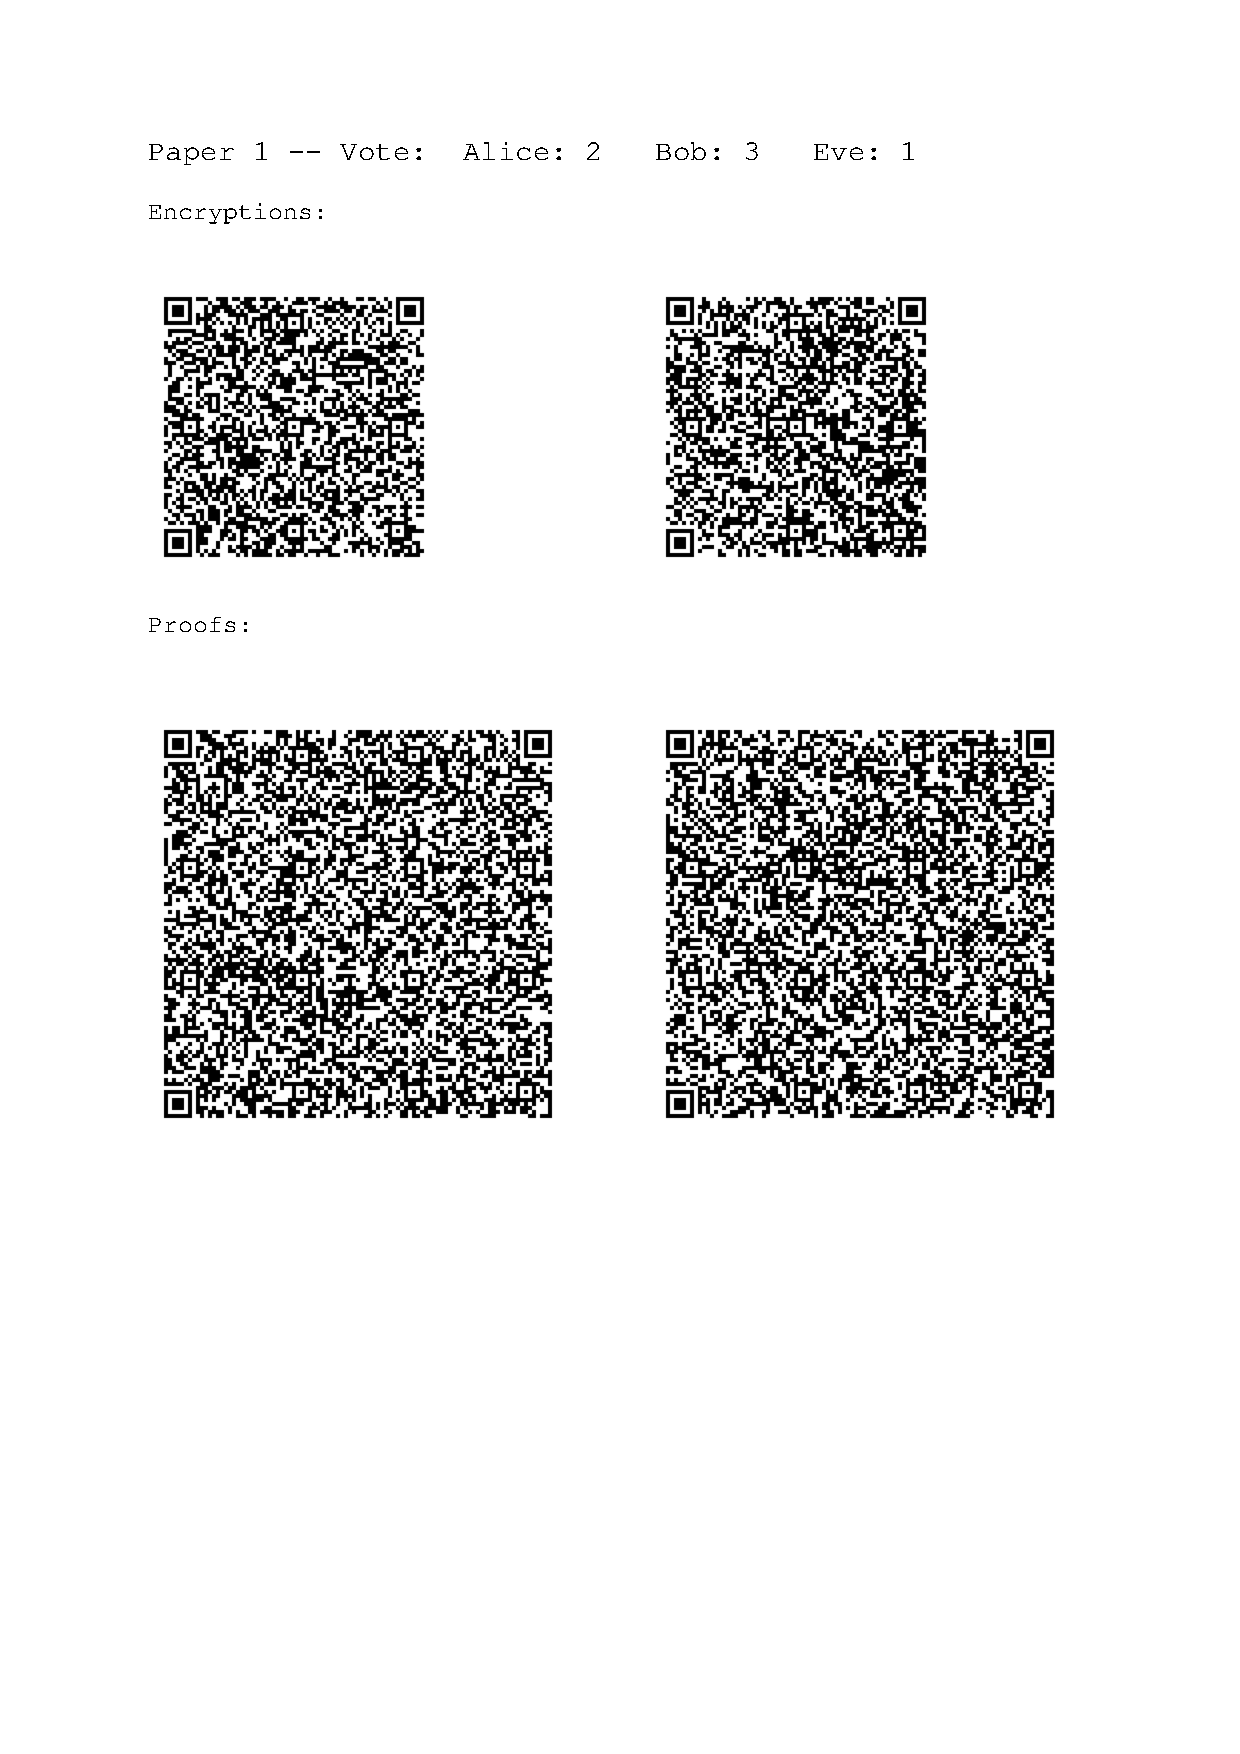
\includegraphics[scale=0.6, trim=2.5cm 10cm 3.1cm 0cm, clip=true]{paper1.pdf}
	\caption{$\Paper_1$: The voter only needs to check the plaintext vote at the top.  This example illustrates a preferential vote: Eve first, Alice next and Bob last.}
	\label{fig:paper1}
\end{figure}

\begin{figure}
	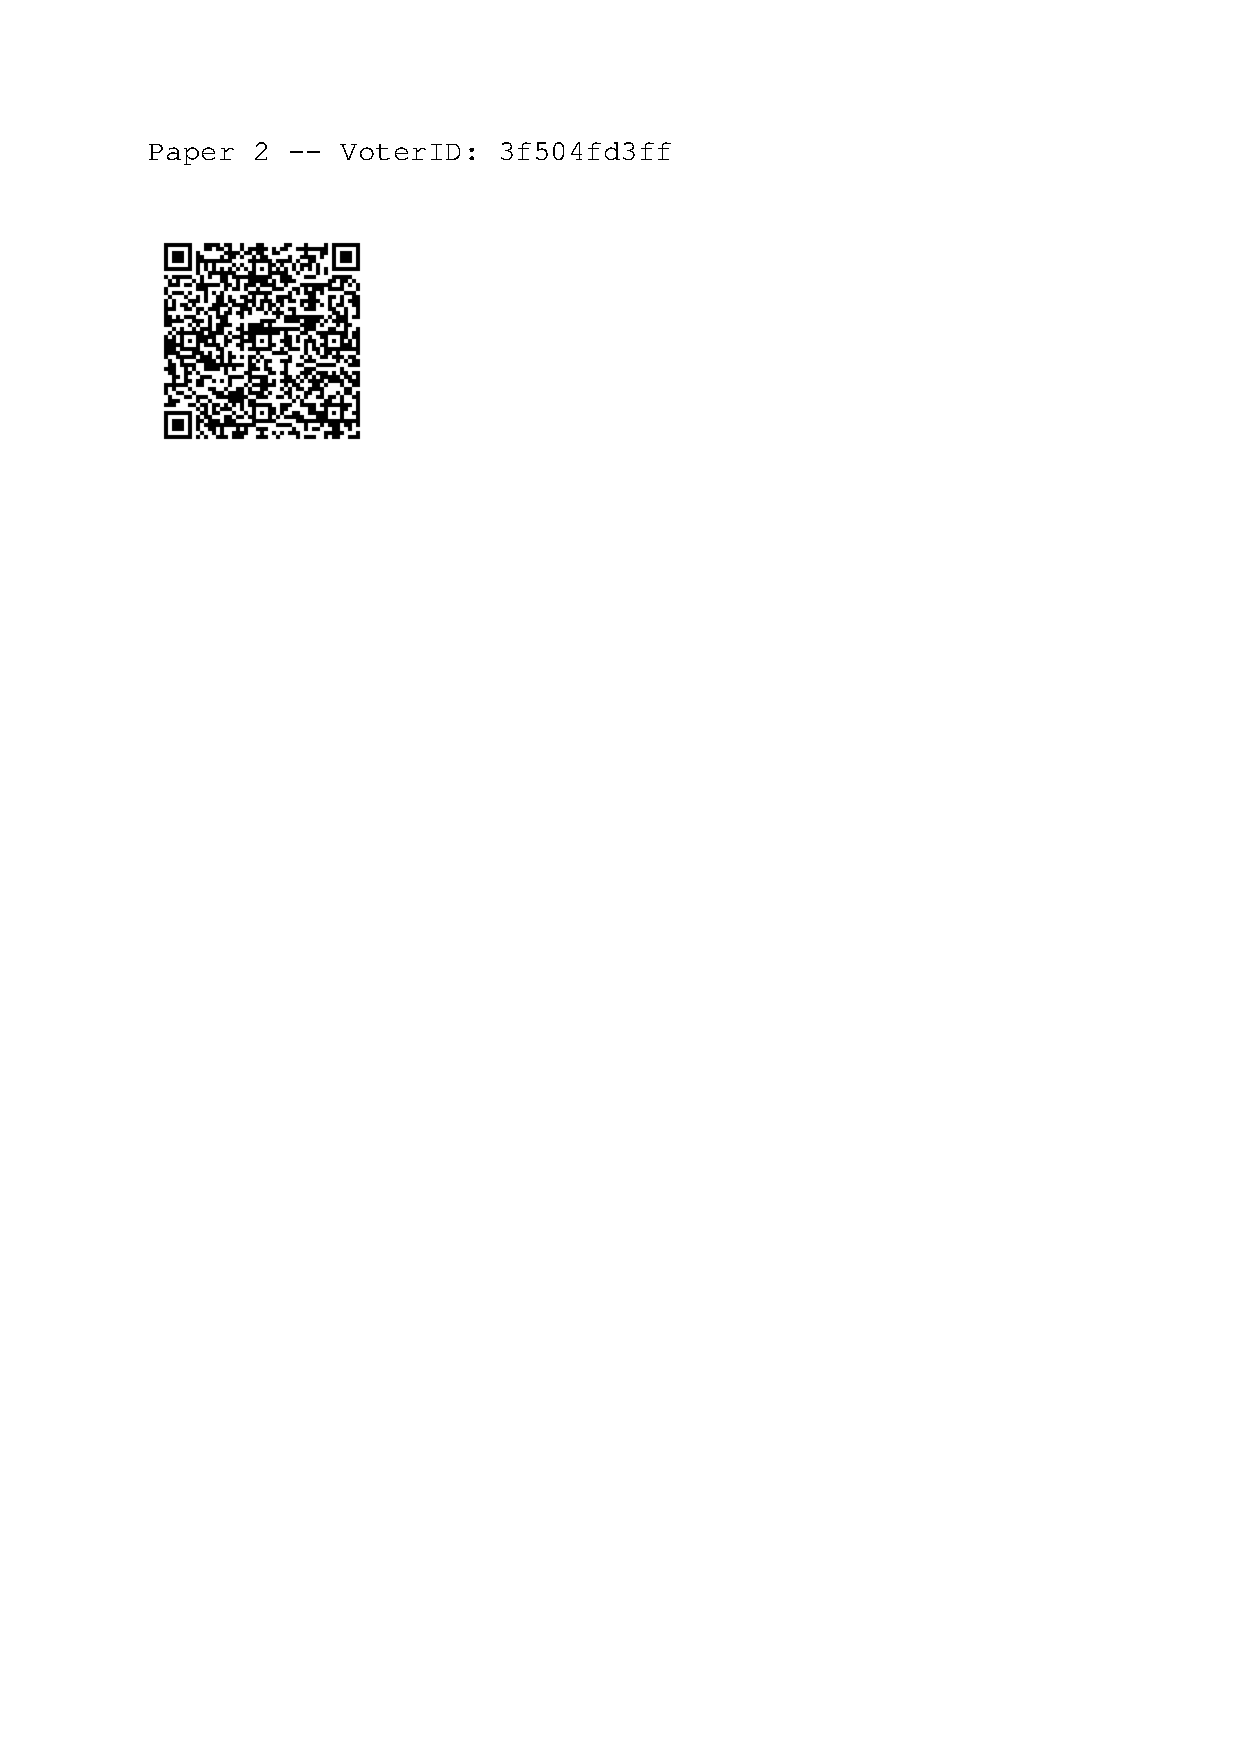
\includegraphics[scale=0.6, trim=0cm 22cm 4cm 0cm, clip=true]{paper2.pdf}
	\caption{$\Paper_2$: The voter only needs to check the plaintext $\VoterID$.}
		\label{fig:paper2}
\end{figure}


\subsection{Tallying ballots}
Once the ballot casting period has ended, the EC can begin receiving ballots. The $\VoterID$ received by the EC is referred to as $\receivedvid$. First, the EC checks the proof on $\Paper_2$. If it fails, they should add it to a list of rejected $\VoterID$s; the same applies for all cryptographic proofs checked by the EC.
They should also confirm that $\receivedvid$ matches the identification on the outside of the envelope. If it does, they should attach the encryption $\{\receivedvid\}_{pk}$ to $\Paper_1$ (without opening it)\footnote{This could be done by \eg tearing the encryption of $\Paper_2$ off and stapling it to $\Paper_1$, or even by providing $\{\receivedvid\}_{pk}$ on a third piece of paper.}, and destroy the rest of $\Paper_2$. The set of $\Paper_1$s from all ballots should now be shuffled physically, to preserve privacy.

After shuffling, the EC receives $\Paper_1$ as:
\begin{align*}
    \Paper_1\ =\ &\big(ReceivedVote,\ \{\receivedvid\}_{pk},\ \{a,b,r_a,r_b\}_{pk},\\
             &\ \PrfKnow(\{a,b,r_a,r_b\}_{pk},\ \mathsf{PrfEnc}(\receivedvid,\ \{\receivedvid\}_{pk})\big)
\end{align*}
The EC should check the proofs, and if they are valid, post the re-randomised received ballot to the WBB. The prior steps should be performed under scrutiny from \eg party representatives to ensure they are faithfully posted; this is the only step that needs active scrutineering.

The trustees next perform a cryptographic mix to produce a list of ballots of the form:
$$\left(\{g^{ReceivedVote}\}_{pk},\ \receivedvid,\ (a,b,r_a,r_b)\right)$$

on the WBB. The resulting list should be joined to the commitments on the WBB by matching $ReceivedVoterID$ to $\VoterID$, producing a list of tuples:
$$\left(\{g^{ReceivedVote}\}_{pk},\ \VoterID,\ (a,b,r_a,r_b), \commit(a;r_a), \commit(b;r_b)\right)$$

Note that we again encrypt $g^{ReceivedVote}$ in the exponent to use the additively homomorphic property later.

If there are multiple tuples for some $\VoterID$, for each tuple the pair of commitments $\commit(a;r_a)$, $\commit(b;r_b)$ should be checked. If the parameters $a,b,r_a,r_b$ are correct openings for \textbf{exactly one} tuple, only that tuple should be accepted; in any other case, no tuples for $\VoterID$ should be accepted.

The accepted tuples should then be matched with the EC's committed encryptions to produce a list of tuples:
$$\left(\{g^{\Vote}\}_{pk},\{g^\Mac\}_{pk}, \{g^{ReceivedVote}\}_{pk},\ \VoterID,\ a, \{g^b\}_{pk}, \PrfEnc(g^b, \{g^b\}_{pk})\right)$$

For all accepted tuples, the electoral trustees should perform a plaintext equivalence test on the WBB to show whether $ReceivedVote=\Vote$ (without decrypting either). If this succeeds, the EC uses the homomorphic properties of ElGamal\footnote{This does not require the secret key, so it can be easily verified by any party.} to construct a second MAC from the received vote:
$$\{g^{\Mac'}\}_{pk}=a\cdot\{g^{ReceivedVote}\}_{pk}\cdot\{g^{b}\}_{pk}$$

where $a\cdot\{g^{ReceivedVote}\}_{pk} = \prod_{i=1}^a \{g^{ReceivedVote}\}_{pk}$. This is posted to the WBB with the $\VoterID$ and the committed vote-MAC pair:
$$\left(\VoterID, \{g^{\Vote}\}_{pk},\ \{g^\Mac\}_{pk},\ \{g^{\Mac'}\}_{pk}\right)$$

The electoral trustees perform another plaintext equivalence test on the WBB to show that $\Mac=\Mac'\ (\bmod\ q)$. For all tuples that pass this test, the electoral trustees should decrypt $\{g^\Vote\}_{pk}$ to produce a final list of valid votes, using the fact that there are only a small number of possible votes to calculate the discrete logarithm. (We assume that once the final list is public, someone counts the votes correctly.)

Note that anybody can check whether a given $\VoterID$ produced a valid vote by seeing whether a tuple $\left(\VoterID, \{g^{\Vote}\}_{pk},\ \{g^{\Mac}\}_{pk},\ \{g^{\Mac'}\}_{pk}\right)$ passed the final plaintext equivalence test, providing \textit{individual} verifiability. It is easy to modify the protocol to remove this property, instead providing \textit{group} verifiability; this may be desirable depending on the application. This alteration and other possible extensions are discussed in Section~\ref{sec-extensions}.
\subsection{The algorithms}
We present a formal description of the procedures that define the protocol for reference below: \textit{Setup} (Algorithm~\ref{alg:setup}), \textit{Cast} (Algorithm~\ref{alg:cast}), and \textit{Tally} (Algorithm~\ref{alg:tally}). Throughout, the $i$th entry in category $cat$ to the WBB is written $\mathcal{B}^{cat}_i$. The set of entries in category $cat$ is written $\mathcal{B}^{cat}$.
\singlespacing
\begin{algorithm}
    \caption{\textit{Setup}$(\lambda)$\textit{:} System setup protocol}
	\begin{algorithmic}[1]
        \LineComment{The following are posted to the WBB:}
        \State $\langle \VoterID \rangle$: a list of IDs of eligible voters.  We assume that these are assigned one-on-one to each voter.
        \State $\mathbb{G} = (g, q)$: the public parameters of an exponential ElGamal encryption scheme.
        (This is additively homomorphic $\bmod\ q$ if the message is in the exponent, where $q$ is the order of $g$ in the group $\mathbb{G}$.)
        \State $pk$: an ElGamal public key generated jointly among the trustees with parameters $\mathbb{G}$ and security parameter $\lambda$. (The corresponding secret key $sk$ is shared among the set of electoral trustees $T$.)
        \State$\mathbb{P} = (G,H,P)$: the public parameters of a perfectly-hiding Pedersen commitment scheme generated such that nobody knows $\dlog_G H$.
    \end{algorithmic}
	\label{alg:setup}
\end{algorithm}
\begin{algorithm}
    \caption{\textit{Cast:} Vote generation and casting protocol}
	\begin{algorithmic}[1]
	\State Device: $a,b,r_a,r_b\leftarrow_R\{1,\ldots,q-1\}$
	\State Device: $c_a\leftarrow\commit(a;r_a), c_b\leftarrow\commit(b;r_b)$
	\State $Device\rightarrow \Wbb$: $\mathcal{B}^{ident}_i=(\VoterID, c_a, c_b)$\label{Step:VoterCommit}
	\State $Voter\rightarrow Device$: $\Vote$
	\State Device: $\Mac\leftarrow a\cdot Vote+b\bmod q$
	\State $Device\rightarrow EC$: $\VoterID, \{g^\Mac\}_{pk}, \{g^\Vote\}_{pk}, \PrfKnow(\{g^\Mac\}_{pk}), \PrfKnow(\{g^\Vote\}_{pk})$% \textit{proofs of knowledge}$
	\State $EC\rightarrow \Wbb$: $\mathcal{B}^{commit}_i=(\VoterID, \rerand\{g^\Mac\}_{pk}, \rerand\{g^\Vote\}_{pk})$ \label{Step:ECPostsVoteMAC}
	\State Device: Wait for $\VoterID$ to appear on WBB
	\State $Device\rightarrow \Paper_1$: $\Vote, \{a,b,r_a,r_b\}_{pk}, \PrfKnow(\{a,b,r_a,r_b\}_{pk})$
	\State $Device\rightarrow \Paper_2$: $\VoterID, \{\VoterID\}_{pk}, \PrfEnc(\VoterID, \{\VoterID\}_{pk})$
	\State $Voter\rightarrow EC$: $\Paper_1, \Paper_2$ (by paper mail)
	\end{algorithmic}
\label{alg:cast}
\end{algorithm}
\begin{algorithm}
    \caption{\textit{Tally:} Vote receiving and tallying protocol}
	\begin{algorithmic}[1]
	\For {$i$th ballot $(\Paper_1,\Paper_2)$ received via paper mail}
		\State $\Paper_2\rightarrow EC:\ \ \receivedvid,\{\receivedvid\}_{pk}, \PrfEnc(\receivedvid,\{\receivedvid\}_{pk})$
		\State EC: $\text{Checks }\receivedvid\text{ matches electoral roll}$
		\State EC: Verifies $\PrfEnc(\receivedvid,\{\receivedvid\}_{pk})$.\par
		\hskip\algorithmicindent On failure, post $\receivedvid$ to $\mathcal{B}^{rejected}$. Skip ballot.\label{Step:ECChecksPrfEnc}
		\State $\Paper_2\rightarrow\Paper_1:\ \{\receivedvid '\}_{pk}$\label{Step:AttachVID}
		\State $\qquad \qquad \qquad\text{Destroy }\Paper_2,\qquad\text{Shuffle }\Paper_1\downarrow$
		\State $\Paper_1\rightarrow EC:\ \ \ReceivedVote, \{\receivedvid\}_{pk},\{a,b, r_a, r_b\}_{pk},\PrfKnow(\{a,b, r_a, r_b\}_{pk})$
		\State EC: $\text{Verifies }\PrfKnow(\{a,b, r_a, r_b\}_{pk})$.\par
		\hskip\algorithmicindent On failure, post $\receivedvid$ to $\mathcal{B}^{rejected}$. Skip ballot.\label{Step:ECChecksPrfKnow}
		\State $\textit{EC} \rightarrow \Wbb : \ \mathcal{B}^{\text{votes}}_i=(\ReceivedVote, \rerand\{\receivedvid\}_{pk},\rerand\{a,b, r_a, r_b\}_{pk})$    \label{Step:ECPostsPaperInfo}
	\EndFor
	\State $T\rightarrow \Wbb: \ \mathcal{B}^{\text{votes'}}=\Mix(\mathcal{B}^{\text{votes}})$\label{Step:MixCast}
	\For {$\mathcal{B}^{\text{votes'}}_i=(\{g^\ReceivedVote\}_{pk}, \{\receivedvid\}_{pk}, \{a,b, r_a, r_b\}_{pk})$}
		\State $T: (a, b, r_a, r_b) = \Dec(\{a,b,r_a,r_b\}_{pk})$\label{Step:DecryptParams}
		\State $T: \receivedvid = \Dec(\{\receivedvid\}_{pk})$\label{Step:DecryptID}
		\State $T\rightarrow \Wbb: \ \mathcal{B}^{\text{mixed}}_i=(\{g^\ReceivedVote\}_{pk}, (a,b, r_a, r_b), \receivedvid, \text{decryption proof})$ \label{Step:RecVoterIDToWBB}
	\EndFor
	\LineComment{Join by matching $\VoterID$ to $\receivedvid$}  \label{Step:FirstWBBMsgs}
	\For {$\mathcal{B}^{\text{mixed}}_i$ such that $\receivedvid$ is unique}
    \LineComment{For this uniqueness test, also include ballots in $\mathcal{B}^{rejected}$}
		%	\State Check that $a,b, r_a, r_b$ is a valid commitment opening of $c_a, c_b$   \& $\{MAC\}_{pk_1} $
		\For {$\mathcal{B}^{\text{ident}}_j=(\VoterID, c_a, c_b)$ such that $\VoterID=\receivedvid$}
			\If {$c_a=\commit(a;r_a)$ and $c_b=\commit(a;r_b)$}
				\State {mark $\mathcal{B}^{\text{ident}}_j$ as a correct commitment opening for $\mathcal{B}^{mixed}_i$}\label{Step:CommitOpening}
			\EndIf
		\EndFor
		\If {exactly one $\mathcal{B}^{\text{ident}}_j$ is a correct opening for $\mathcal{B}^{\text{mixed}}_i$}
			
			% The below check ensures the EC didn't falsify the MAC commitment.
			% In particular, it's important we construct MAC' from the {Vote}_{pk} committed to by the EC.  
			\label{Step:uniqueCommitOpen}
			\State $\Wbb\rightarrow T:\ \mathcal{B}^{\text{commit}}_k=(\VoterID, \{g^\Vote\}_{pk}, \{g^\Mac\}_{pk})$\par
			\hspace{1cm}{If there is no $\mathcal{B}^{\text{commit}}_k$ with matching $\VoterID$, proceed to the next iteration.}
			\State $T\rightarrow \Wbb: \pet\big(\{g^\ReceivedVote\}_{pk}, \{g^\Vote\}_{pk}\big)$\label{Step:ECVotePEP}
			\State $\{g^{\Mac'}\}_{pk} := a \cdot \{g^\Vote\}_{pk} + \{g^b\}_{pk}$
			\State $T\rightarrow \Wbb: \pet\big(\{g^\Mac\}_{pk},\{g^{\Mac'}\}_{pk}\big)$\label{Step:ECMACPEP}
			\If{plaintext equivalence proofs pass}
				\State $T\rightarrow \Wbb:\ \mathcal{B}^{\text{accepted}}_i = \left(\VoterID, \{g^\Vote\}_{pk}\right)$\label{Step:PETsPassed}

			\EndIf
		\EndIf
	\EndFor
	\State $T\rightarrow \Wbb: \mathcal{B}^{accepted'}=\Mix(\mathcal{B}^{\text{accepted}})$\label{Step:MixAccepted}
	\LineComment{Produce final tally}
	\For {$\mathcal{B}^{\text{accepted'}}_i=\{g^\Vote\}_{pk}$ on $\Wbb$}
		\State $T\rightarrow \Wbb: \mathcal{B}^{\text{tally}}_i=\Dec(\{g^\Vote\}_{pk})$\label{Step:DecryptVote}
	\EndFor
	\end{algorithmic}
\label{alg:tally}
\end{algorithm}
\onehalfspacing
\newpage
\subsection{Verification procedure}
Verification is broken into three main areas. Firstly, each voter must check the paper printout herself to make sure it correctly reflects her vote, and she must also check whether her ID appears in the final mix. Secondly, scrutineers from third parties must observe the process of receiving paper ballots. Finally, the WBB transcript can in theory be verified by anyone; because this may not be a trivial computational task, we expect that trusted entities such as media organisations would perform verification of this transcript on voters' behalf.

One of the great challenges in paper elections is \textit{chain-of-custody}: once a paper ballot is filled out by a voter, it should never leave the sight of a trusted authority. Traditional postal voting breaks this requirement, as postal channels are demonstrably vulnerable to interception~\cite{stewart2010losing}. To address this issue, our protocol defines a weaker trust model than the traditional chain of custody. The protocol is verifiable as long as at least one of the below is honest:
\begin{itemize}
    \item the client's device
    \item the postal channel and the electoral commission
\end{itemize}
Thus an adversary can undetectably cheat in the election if they control both the device and the postal channel (and/or the electoral commission), but cannot win if they control only one. This strikes a reasonable compromise, since if the EC (or postal service) deliberately compromises voters' devices, this is indicative of systemic corruption that no cryptographic verification scheme can address.

\paragraph{By election scrutineers.} Scrutineers present when the received envelopes are opened must check:
\begin{enumerate}
    \item that the received $\VoterID$ matches the entry on the electoral roll;
    \item that the proof of encryption on $\Paper_2$ is correct;
    \item that the encryption on $\Paper_2$ was correctly attached to $\Paper_1$; and
    \item that the vote posted on the WBB matches the vote on $\Paper_1$.
\end{enumerate}
This procedure mirrors that already in widespread use for traditional postal votes, and can be easily carried out with a quick visual inspection, perhaps using a mobile app to check the proof of encryption.

\paragraph{By the voter.} Before sending their vote by mail, the voter \textbf{must} check that the printed vote matches the vote they intend to cast, and that the printed $\VoterID$ is theirs.\footnote{It should be overwhelmingly unlikely that two $\VoterID$s can be almost but not quite the same, \eg by using a hash function indistinguishable from uniform randomness.} If they do not perform these checks, their vote can be undetectably substituted for another.

Once the receiving and tallying process is complete, the voter \textbf{should} check that their $\VoterID$ appears in the accepted list $\mathcal{B}^{accepted}$ on the WBB, and either carry out the full WBB verification themselves (Algorithm~\ref{alg:globalverify}) or check that a trusted organisation has done it for them. If the voter \textbf{does not} perform these check, the election integrity can still be assured by others; however, the voter themselves will have no certainty.

A full description of the voter's verification procedure appears in $\textit{VoterVerify}$ (Algorithm~\ref{alg:voterverify}) below. We also provide $\textit{GlobalVerify}$ (Algorithm~\ref{alg:globalverify}) describing the full set of verifications to perform on the WBB records. Note that the voter verification algorithm is defined independently of the global verification algorithm, to simplify modelling.

\singlespacing
\begin{algorithm}
    \caption{\textit{VoterVerify:} Protocol for verification by the voter}
	\begin{algorithmic}[1]
        \State Check that the vote on $\Paper_1$ matches the intended vote
        \State Check that the $\VoterID$ on $\Paper_2$ is correct
        \LineComment{Once the election is complete}
        \State Check that the voter's $\VoterID$ appears in some row of $\mathcal{B}^{\text{accepted}}$
        \If {the above checks succeed}
            \State \Return $\mathsf{accept}$
        \Else
            \State \Return $\mathsf{reject}$
        \EndIf
    \end{algorithmic}
	\label{alg:voterverify}
\end{algorithm}
\begin{algorithm}
    \caption{\textit{GlobalVerify:} Global verification protocol for the WBB}
	\begin{algorithmic}[1]
        \State Verify the mix proof for $\mathcal{B}^{\text{votes}'}$ in Step 10 of \textit{Tally}\label{step:verify-mix}
        \State Verify the decryption proofs in Steps 12 and 13 of \textit{Tally}\label{step:verify-decrypt}
        \State Verify all PET proofs in Steps 23 and 25 of \textit{Tally}\label{step:verify-pets}
        \State Verify the mix proof for $\mathcal{B}^{\text{accepted}'}$ in Step 10 of \textit{Tally}\label{step:verify-mix2}
        \State Verify the decryption proofs in Step 31 of \textit{Tally}\label{step:verify-decrypt2}

        \For {each row $\mathcal{B}^{\text{accepted}}_i = (\VoterID, \{g^{\Vote}\}_{pk})$}
            \State Verify that $\VoterID$ is unique in $\mathcal{B}^{\text{mixed}}
            $ and does not appear in $\mathcal{B}^{\text{rejected}}$\label{step:verify-voterid}
            \State Verify that exactly one commitment $\mathcal{B}^{\text{ident}}_j=(\VoterID, c_a, c_b)$ has a correct opening in $\mathcal{B}^{\text{mixed}}$ such that $\VoterID=\receivedvid$\label{step:verify-opening}
            \State Verify that the PETs in Steps 23 and 25 of \textit{Tally} pass\label{step:verify-pet-pass}
        \EndFor
        \If {the above checks succeed}
            \State \Return $\mathsf{accept}$
        \Else
            \State \Return $\mathsf{reject}$
        \EndIf
    \end{algorithmic}
	\label{alg:globalverify}
\end{algorithm}
\onehalfspacing
\subsection{Interpreting the outcome}\label{sec-outcome}
After the protocol is carried out and verified, we have two separate vote records: one from the paper ballots, and the other from $\mathcal{B}^{\text{tally}}$. Interpreting the results correctly is not entirely straightforward; in this section we discuss how to correctly interpret the results in light of the fact that there may have been attempts to manipulate the process.

At the end of the election, the WBB contains four sets of $\VoterID$s:
\begin{enumerate}
    \item $\mathcal{L}^{\text{registered}}$: a list of registered $\VoterID$s drawn from $\mathcal{B}^{\text{ident}}$, \ie those who have uploaded a $\VoterID$ and commitments

    \item $\mathcal{L}^{\text{received}}$: a list of received $\VoterID$s drawn from $\mathcal{B}^{\text{votes}}$, \ie those whose ballots were posted by the EC in Step 9 of \textit{Tally}

    \item $\mathcal{L}^{\text{rejected}}$: a list of rejected $\VoterID$s drawn from $\mathcal{B}^{\text{rejected}}$, \ie those whose ballots arrived with invalid proofs

    \item  $\mathcal{L}^{\text{accepted}}$: a list of accepted $\VoterID$s drawn from $\mathcal{B}^{\text{tally}}$, \ie those whose ballots uniquely and exactly matched a registered $\VoterID$'s commitments
\end{enumerate}

Clearly if $\mathcal{L}^{\text{accepted}}$ is not a subset of $\mathcal{L}^{\text{registered}} \cup \mathcal{L}^{\text{rejected}}$, then something has gone badly wrong and verification should fail. However, in the normal course of an election we expect some deviation between these sets: some voters may register but never vote, some votes may go missing in the mail, and some votes may be recorded incorrectly on arrival. We would like to define an ``acceptable'' election outcome in such a way that we detect fraud but do not cause the election to fail in the case of small deviations.

First, the votes from the $\VoterID$s in $\mathcal{L}^{\text{accepted}}$ are those for which everything worked perfectly, and should be accepted. If they deviate from the paper record, this indicates one type of problem: substitution of paper ballots in the mail (or by the EC after arrival). Another type of problem is that of voters who registered but do not have a unique matching commitment at Step 21 of \textit{Tally}, or did not pass PETs in Steps 23 or 25 of Tally. Depending on the specific nature of the problem, this could be evidence of attempted fraud (\eg multiple commitment openings could indicate the voter's device has been compromised), or it could be a legitimate decision to register but not vote.

In summary, $\mathcal{L}^{\text{accepted}}$ provides an arguable election outcome, while the other lists provide some indication of the amount of error or manipulation attempts. We will call the amount of detected error $\varepsilon = |\mathcal{L}^{\text{registered}} \cup \mathcal{L}^{\text{received}}| - |\mathcal{L}^{\text{accepted}}|$, and call the accepted error $\delta$. Let $\mathcal{O}$ be the outcome of the election with margin $M$ according to the paper record. For example, in a simple first-past-the-post election $\mathcal{O}$ would be a vector of vote counts for each candidate and $M$ would be the difference in the number of accepted votes for the top two candidates. Finally, given a WBB transcript $\tau$ define the acceptable number of errors to be $d$.

One obvious formula would be: accept the outcome $\mathcal{O}$ if the plaintext ballots give the same winner as $\mathcal{L}^{\text{accepted}}$, \ie $\delta = M$. Another would be: accept $\mathcal{O}$ if the demonstrated error was below the margin, ignoring those voters who registered but for whom a vote was not received, \ie $\delta = M + |\mathcal{L}^{\text{registered}}| - |\mathcal{L}^{\text{received}}|$.

We abstract these choices away by defining the result of the transcript $\tau$ given the outcome $\mathcal{O}$ and the accepted error $\delta$ to be

$$\mathsf{Result}(\tau) =
\begin{cases}
    \mathcal{O} & \text{if } \varepsilon < \delta \text{ and } \mathit{GlobalVerify}(\tau) \text{ passes} \\
    \bot        & \text{otherwise}
\end{cases}$$

where $\bot$ indicates an erroneous outcome. To be confident that there were at most $\delta$ detected errors, at least $\theta = |\mathcal{V}| - (M - \delta)$ voters must correctly verify their votes (where $\mathcal{V}$ is the set of voters). Thus there is an inverse relationship between the allowed deviation and the number of voters that are allowed to not perform verification.
\newpage
\section{Properties of the protocol}\label{sec-properties}
\subsection{Privacy}
Any practical voting scheme needs to guarantee the privacy of its voters. To be more precise, it should not be possible for anybody to determine which vote was cast by a particular voter except the voter themselves. Postal voting demands that voters' identities be verified on receipt of the vote; this means that the electoral commission could in principle break a voter's privacy. However, real-world postal voting systems have steps in place to preserve voters' privacy. For example, in Australian elections voters' identities are checked by having the voter write their name and address on the envelope, and fold their ballot before placing it inside. In this way, the voter's identity can be verified, then the envelope can be opened and the still-folded ballot can be passed to somebody who did not learn the voter's identity. Our protocol involves a similar procedure. Privacy is distinct from receipt freeness, which demands that a voter not be able to prove which vote they cast to anybody else.

Our definition of privacy is based on that of~\cite{kiayias2015end}, though we separate voter privacy from receipt freeness because we can prove privacy against a stronger adversary than for receipt freeness. For privacy, we will remove the simulator defined by~\cite{kiayias2015end}---the purpose of the simulator is to allow a voter to lie about their vote, which is not relevant in the privacy-only case.

Voter privacy is defined as a game between a PPT adversary $\mathcal{A}$ and a challenger $\mathcal{C}$. We consider a set of $m$ candidates $\mathcal{P}=\{P_1,\ldots,P_m\}$, a set of $n$ voters $\mathcal{V}=\{V_1,\ldots,V_n\}$, a set of allowed candidate selections $\mathcal{U}$, and an \textit{election evaluation function} $f : \mathcal{U}^n \to \mathbb{N}^m$ mapping the voters' candidate selections to a vector where the $i$th index contains the number of votes for candidate $\mathcal{P}_i$ (or perhaps a vector of preference numbers for preferential systems). The intuition is that the adversary chooses the parameters for the election and may choose to \textit{corrupt} a number of voters of its choice, meaning that it acts as the voter. The challenger acts as the EC, WBB, and election trustees, and acts on behalf of honest voters; for each non-corrupted voter, the adversary provides the challenger with two votes to choose from. The adversary wins if it is able to guess which of the two votes the non-corrupted voters cast \textbf{and} the adversary did not choose the parameters such that it always wins.

\begin{definition}[Voter privacy]
    Consider the below game between an adversary $\mathcal{A}$ and a challenger $\mathcal{C}$, written $G^\mathcal{A}_{\text{Privacy}}(1^\lambda, n, m)$.
    \begin{enumerate}
        \item Given parameters $1^\lambda, n, m$, the adversary $\mathcal{A}$ chooses a set of candidates $\mathcal{P}=\{P_1,\ldots,P_m\}$, voters $\mathcal{V}=\{V_1,\ldots,V_n\}$, and candidate selections $\mathcal{U}$. It sends the sets $\mathcal{P}, \mathcal{V},$ and $\mathcal{U}$ to $\mathcal{C}$.
        \item $\mathcal{C}$ flips a coin $b\in\{0, 1\}$, and runs \textit{Setup}$(\lambda)$ to obtain parameters for ElGamal encryption and Pedersen commitments. It sends the public parameters to $\mathcal{A}$.
        \item $\mathcal{A}$ schedules the $\mathit{Cast}$ protocol for all voters, which are allowed to run concurrently. For all $V_l\in\mathcal{V}$, the adversary chooses whether $V_l$ is to be corrupt. $\mathcal{C}$ acts as the EC.
        \begin{itemize}
            \item If $V_l$ is corrupt, $\mathcal{A}$ acts on $V_l$'s behalf as it wishes.
            \item If $V_l$ is honest, $\mathcal{A}$ sends two candidate selections $\mathcal{U}_l^0, \mathcal{U}_l^1 \in \mathcal{U}$ to $\mathcal{C}$. It must do so such that $f(\langle\mathcal{U}_l^0\rangle_{V_l\in \tilde{\mathcal{V}}})=f(\langle\mathcal{U}^1_l)_{V_l\in \tilde{\mathcal{V}}}\rangle$ where $\tilde{\mathcal{V}}$ is the set of honest voters (that is, the set of honest votes alone does not leak $b$). $\mathcal{C}$ acts on $V_l$'s behalf to cast the vote $\mathcal{U}_l^b$. During this process $\mathcal{A}$ may view the encrypted data $\{g^{\Vote}\}_{\mathit{pk}}, \{g^{\Mac}\}_{\mathit{pk}}$ in transit to the EC, as well as the WBB and $\Paper_1, \Paper_2$ (after shuffling).
            
            We require that the relationship between $\Paper_1$ and $\Paper_2$ defined by the shared encryption $\{\VoterID\}_{pk}$ is forgotten. After $\textit{Cast}$ terminates, $\mathcal{C}$ provides to $\mathcal{A}$ the receipt consisting of the $\VoterID$ for $V_l$ (and thus the data on the WBB indexed by the $\VoterID$).
        \end{itemize}
        \item $\mathcal{C}$ runs the $\mathit{Tally}$ protocol, acting as the EC, the trustee set $T$, and the WBB. $\mathcal{A}$ may continue to observe the WBB.
        \item $\mathcal{A}$ outputs a bit $b^*$.
    \end{enumerate}
    $\mathcal{A}$ wins the game if and only if $b=b^*$. A scheme achieves \textit{voter privacy} if for all PPT adversaries $\mathcal{A}$, $\Adv\left(G^\mathcal{A}_{\text{Privacy}}(1^\lambda, n, m)\right)=\negl(\lambda)$.
\end{definition}

This definition contains some very careful phrasing. Note first what the adversary is allowed to learn: it can see anything on the WBB, anything on $\Paper_2$ for all voters, anything on $\Paper_1$ for all voters (but \textbf{not} which $\Paper_2$ corresponds to the $\Paper_1$ for honest voters), and any of the encrypted data sent to the EC (but \textbf{not} an honest voter's view of how it was constructed). This is more general than what we will allow for receipt-freeness.

It is worth discussing some details in the condition placed on the adversary's choice of candidate selections in step 3. This prevents any attempt by the adversary to trivialise the problem by forcing the election's outcome alone to reveal $b$, and in particular prevents the adversary choosing all but one voter to be corrupt---since the list of decrypted votes on the WBB would reveal the cast vote. This is important since the protocol reveals not only the winner of the election, but also a full list of all valid votes.

A proof that our scheme satisfies this property follows. The goal will be to sequentially alter the privacy game, where each step is negligibly distinguishable from the previous step so that the adversary does not notice the manipulations. We will arrive at a game where none of the ciphertexts contain any information, so the adversary has no hope of winning.

\begin{theorem}\label{thm-privacy}
    Assume the EC and voter's device are honest as well as a threshold of electoral trustees. For all constants $m \in \mathbb{N}$ and $n=\poly(\lambda)$, the voting system described in Section~\ref{sec-protocol} satisfies voter privacy.
\end{theorem}
\begin{proof}
    We first summarise some key facts. During \textit{Cast}, the adversary sees:
    \begin{itemize}
        \item $(\VoterID, c_a, c_b)$
        \item $(\VoterID, \{g^{\Vote}, g^{\Mac}\}_{pk}, \mathsf{PrfKnow}(\{g^{\Vote}, g^{\Mac}\}_{pk}))$
        \item $(\VoterID, \mathsf{Rerand}(\{g^{\Mac}, g^{\Vote}\}))$
    \end{itemize}

    During \textit{Tally}, the adversary sees:
    \begin{itemize}
        \item $(\VoterID, \{\VoterID\}_{pk}, \text{encryption proof})$
        \item $(\Vote, \{\VoterID\}_{pk}, \{a, b, r_a, r_b\}_{pk}, \mathsf{PrfKnow}(\{a, b, r_a, r_b\}_{pk}))$
        \item $(\ReceivedVote, \mathsf{Rerand}(\{\receivedvid\}_{pk}), \mathsf{Rerand}(\{a, b, r_a, r_b\}_{pk}))$
        \item $(\{\ReceivedVote\}_{pk}, (a, b, r_a, r_b), \receivedvid, \text{decryption proofs})$
        \item $(\Vote, \text{decryption proof})$
    \end{itemize}

    Crucially, the adversary cannot use $\{\VoterID\}_{pk}$ in the above to link $\VoterID$ and $\Vote$ since we require the relationship is forgotten by detaching the encryption from the rest of $\Paper_2$, attaching it to $\Paper_1$, and shuffling before opening $\Paper_1$.

    We will use a hybrid argument to construct a sequence of games until we arrive at one in which the adversary clearly cannot have any advantage.
    \begin{itemize}[leftmargin=4em]
        \item[Game] $G_0$: the unaltered game $G^\mathcal{A}_{\text{Privacy}}(1^\lambda, n, m)$. By definition $\Adv_{G_0, G^\mathcal{A}_{\text{Privacy}}(1^\lambda, n, m)}(\mathcal{A})=0$.
        
        \item[Game] $G_1$: the same as Game $G_0$, except the decryption and PETs on the WBB are simulated using knowledge of their plaintexts rather than the decryption key; this is possible since every ciphertext is either generated by the challenger, or is generated by the adversary with an accompanying ZKP proving knowledge (so the challenger can use the corresponding zero-knowledge extractor). The soundness error in the adversary's ZKPs gives $\Adv_{G_1, G_0}(\mathcal{A})=\negl(\lambda)$.
 
        \item[Game] $G_2$: the same as Game $G_1$, except the ZKPs used to prove correctness of the decryptions and PETs are simulated via the zero-knowledge simulator. The ZKPs are non-malleable and the WBB filters for duplicates, so the adversary's proofs cannot depend on the simulated proofs---we are therefore still able to use the extractor from Game $G_1$. Note that the challenger no longer uses the ElGamal secret key for any purpose. The simulator has no error, so $\Adv_{G_2, G_1}(\mathcal{A})=0$.
 
        \item[Game] $G_3$: the same as Game $G_2$, except the mixing proofs are also simulated via the zero-knowledge simulator to ensure no information about the permutation or randomness used is leaked. As in $G_2$, we have $\Adv_{G_3, G_2}(\mathcal{A})=0$.
        
        \item[Game] $G_4$: the same as Game $G_3$, except the ciphertexts are replaced with encryptions of random values from an oracle (and re-randomisations are replaced with fresh encryptions of random values). No ciphertexts are ever decrypted, so we can use the IND-CPA property of ElGamal\footnote{If we did decrypt ciphertexts, the adversary could learn the decryptions of certain ciphertexts and use this to undermine the IND-CPA property.} to guarantee that $\Adv_{G_4,G_3}(\mathcal{A})=\negl(\lambda)$ (because the adversary cannot tell the ciphertexts were replaced).
    \end{itemize}
    In Game $G_4$, the encryptions are random and contain no usable information aside from the (decoupled) $\VoterID$s and $\Vote$s. The link between $\VoterID$ and $\Vote$ is destroyed by the mixing; assuming honesty of at least one mixing trustee and $n - k + 1$ decrypting trustees, the adversary cannot have any advantage in guessing which vote was cast by each voter. Therefore, $\Adv(\mathcal{A}, G_3)=0$, which implies $\Adv\left(G^\mathcal{A}_{\text{Privacy}}(1^\lambda, n, m)\right)=\negl(\lambda)$ as required.
\end{proof}
\subsection{Receipt-freeness}
The game we use for receipt-freeness will be similar to the privacy game, with two key differences:
\begin{enumerate}
    \item The adversary's view is restricted to the WBB and the view of the voter's client (\textbf{not} the pieces of paper).
    \item The voter has access to a simulator algorithm $\mathcal{S}$ that can \textit{simulate} their client's view to support a claim that they submitted a different vote.
\end{enumerate}

Consider a coercer who does not collude with the EC, but makes demands of the voter and their client. We will prove \textit{passive} receipt-freeness, meaning that we assume the voter and client follow the protocol honestly aside from recording all of their secrets. We must further assume the channel between the voter and EC is not tapped by the coercer; this models a coercer who does not have the capacity to intercept encrypted communications such as TLS over the Internet.\footnote{TLS is \textbf{not} untappable: a voter could prove what they sent by revealing their AES key generated in the TLS handshake.} (At least one untappable channel in one direction is necessary and sufficient for receipt-freeness~\cite{hirt2000efficient}. We use two, and do not consider a cheating EC.)

The coercer demands the voter casts some vote $\Vote_{\text{cr}}$ and provides the coercer with a transcript describing the setup, ballot generation, and ballot casting for $\Vote_{\text{cr}}$. The voter will evade coercion (to submit a different vote $\Vote$) by telling the truth about their secrets $a, b, r_a, r_b$ but claiming to have sent a different MAC $\Mac_{\text{cr}} = a\cdot \Vote_{\text{cr}} + b \bmod q$. This relies on the fact that the EC posts a re-randomised encryption of the voter's true MAC $\Mac = a \cdot \Vote + b \bmod q$, which is indistinguishable from a re-randomised encryption of $\Mac_{\text{cr}}$.

Our definition of receipt-freeness follows.
\begin{definition}[Receipt-freeness]
    Consider the below game between an adversary $\mathcal{A}$ and a challenger $\mathcal{C}$, written $G_{\text{Rec-free}}^{\mathcal{A},\mathcal{S}}(1^\lambda, n, m)$.
    \begin{enumerate}
        \item Given $1^\lambda, n, m$, $\mathcal{A}$ chooses a set of candidates $\mathcal{P}=\{P_1,\ldots,P_m\}$, voters $\mathcal{V}=\{V_1,\ldots,V_n\}$, and candidate selections $\mathcal{U}$. It sends the sets $\mathcal{P}, \mathcal{V},$ and $\mathcal{U}$ to $\mathcal{C}$.
        \item $\mathcal{C}$ tosses a coin $b\in\{0, 1\}$, and runs the $\mathsf{Setup}$ protocol to obtain parameters for ElGamal encryption and Pedersen commitment. It sends the public parameters to $\mathcal{A}$.
        \item $\mathcal{A}$ schedules the $\mathit{Cast}$ protocol for all voters, which are allowed to run concurrently. For all $V_l\in\mathcal{V}$, the adversary chooses whether $V_l$ is to be \textit{corrupt} or \textit{honest}. $\mathcal{C}$ plays the role of the EC.
        \begin{itemize}
            \item If $V_l$ is corrupt, $\mathcal{A}$ acts on $V_l$'s behalf as it wishes.
            \item If $V_l$ is honest, $\mathcal{A}$ sends two candidate selections $\mathcal{U}_l^0, \mathcal{U}_l^1 \in \mathcal{U}$ to $\mathcal{C}$. It must do so such that $f(\langle\mathcal{U}_l^0\rangle_{V_l\in \tilde{\mathcal{V}}})=f(\langle\mathcal{U}^1_l)_{V_l\in \tilde{\mathcal{V}}}\rangle$ where $\tilde{\mathcal{V}}$ is the set of honest voters (that is, the set of honest votes alone does not leak $b$). $\mathcal{C}$ acts on $V_l$'s behalf to cast the vote $\mathcal{U}_l^b$. During this process $\mathcal{A}$ may view \textbf{only} the WBB. After $\mathit{Cast}$ terminates, $\mathcal{C}$ provides to $\mathcal{A}$:
            \begin{enumerate}
                \item the \textit{receipt} $\alpha_l$ consisting of voter $V_l$'s $\VoterID$
                \item if $b=0$, $V_l$'s real view (including randomness for the encryptions)
                \begin{gather*}
                    a, b, r_a, r_b, \Vote=\mathcal{U}^0_l, \Mac,\\\{g^\Vote\}_{pk}, \{g^\Mac\}_{pk}, \{a,b,r_a,r_b\}_{pk},\{\VoterID\}_{pk}
                \end{gather*}
                If $b=1$, $\mathcal{C}$ instead provides a simulated view using $\mathcal{S}$.
            \end{enumerate}
        \end{itemize}
        \item $\mathcal{C}$ runs the $\mathit{Tally}$ protocol, acting as the EC, the trustee set $T$, and the WBB. $\mathcal{A}$ may continue to observe the WBB.
        \item $\mathcal{A}$ outputs a bit $b^*$.
    \end{enumerate}
    $\mathcal{A}$ wins the game if and only if $b=b^*$. A scheme achieves \textit{receipt freeness} if there exists a simulator $\mathcal{S}$ such that for all PPT adversaries $\mathcal{A}$
    $$\Adv\left(\mathcal{A}, G^{\mathcal{A},\mathcal{S}}_{\text{Rec-free}}(1^\lambda, n, m)\right)=\negl(\lambda)$$
\end{definition}

\begin{theorem}\label{thm-Rec-free}
    Assume the adversary does not collude with the EC, and cannot tap the channel between the voter and EC. For all constants $m \in \mathbb{N}$ and $n=\poly(\lambda)$, the voting system described in Section~\ref{sec-protocol} satisfies receipt freeness.
\end{theorem}
\begin{proof}
    First, we recall the information visible to the adversary. During \textit{Cast}, the adversary sees
    
    \begin{itemize}
        \item $(\VoterID, c_a, c_b)$
        \item $(\VoterID, \mathsf{Rerand}(\{g^{\Mac}\}_{pk}), \mathsf{Rerand}(\{g^{\Vote}\}_{pk}))$
    \end{itemize}

    After \textit{Cast}, the adversary sees the voter's (possibly-simulated) view
    \begin{gather*}
        a, b, r_a, r_b, \Vote, \Mac,\\\{g^\Vote\}_{pk}, \{g^\Mac\}_{pk}, \{a,b,r_a,r_b\}_{pk},\{\VoterID\}_{pk}
    \end{gather*}

    During \textit{Tally}, the adversary sees
    \begin{itemize}
        \item $(\ReceivedVote, \mathsf{Rerand}(\{\receivedvid\}_{pk}), \mathsf{Rerand}(\{a, b, r_a, r_b\}_{pk}))$
        \item $(\{\ReceivedVote\}_{pk}, (a, b, r_a, r_b), \receivedvid, \text{decryption proofs})$
        \item $(\Vote, \text{decryption proof})$
    \end{itemize}

    Now we define the simulator. $\mathcal{S}$ receives an honest voter's view
    \begin{gather*}
        a, b, r_a, r_b, \Vote=\mathcal{U}^1_l, \Mac,\\\{g^\Vote\}_{pk}, \{g^\Mac\}_{pk}, \{a,b,r_a,r_b\}_{pk},\{\VoterID\}_{pk}
    \end{gather*}
    It computes a valid MAC for the claimed vote $\mathcal{U}^0_l$ as well as ciphertexts for the claimed vote and MAC. It then outputs the simulated view
    \begin{gather*}
        a, b, r_a, r_b, \Vote_{\text{cr}}=\mathcal{U}^0_l, \Mac_{\text{cr}}=a\cdot\Vote'+b,\\\{g^{\Vote_{\text{cr}}}\}_{pk}, \{g^{\Mac_{\text{cr}}}\}_{pk}, \{a,b,r_a,r_b\}_{pk},\{\VoterID\}_{pk}
    \end{gather*}

    We will use a hybrid argument to prove the result as per Theorem~\ref{thm-privacy}.
    \begin{itemize}[leftmargin=4em]
        \item[Game] $G_0$: The actual game $G^{\mathcal{A},\mathcal{S}}_\text{Rec-free}(1^\lambda,n,m)$, where the challenger uses $\mathcal{U}^b_l$ in the $\mathit{Cast}$ protocol and the above simulator is invoked when $b=1$.  (That is, voters vote as they wish and run the coercion-resistance strategy.)
        
        By definition $\Adv_{G_0,G^{\mathcal{A},\mathcal{S}}_{\text{Rec-free}}(1^\lambda,n,m)}(\mathcal{A}) = 0$.
    
        \item[Game] $G_1$: The same as Game $G_0$, except the decryption and PETs are simulated with knowledge of the plaintext as in Theorem~\ref{thm-privacy}; $\Adv_{G_1, G_0}(\mathcal{A})=\negl(\lambda)$.
    
        \item[Game] $G_2$: The same as Game $G_1$, except the proofs used to demonstrate correct decryption and plaintext equivalence are simulated with their zero-knowledge simulators as in Theorem~\ref{thm-privacy}. Note that as before we no longer use the ElGamal secret key for any purpose. We then have $\Adv_{G_2, G_1}(\mathcal{A})=0$.
 
        \item[Game] $G_3$: The same as Game $G_2$, except the proof of correct mixing is simulated as in Theorem~\ref{thm-privacy}. To ensure the link between successive ciphertexts is destroyed, the challenger uses knowledge of the plaintext to replace ciphertexts with fresh encryptions after each mix. We have $\Adv_{G_3, G_2}(\mathcal{A})=0$.
    
        \item[Game] $G_4$: The same as Game $G_3$, except when $b = 1$:
        \begin{enumerate}
            \item In Step 7 of $\mathit{Cast}$, the challenger posts an encryption of the claimed MAC $\{g^{\Mac_{\text{cr}}}\}_{pk}$ instead of a re-randomised encryption of the actual MAC $\{g^\Mac\}_{pk}$.
            \item In Step 9 of $\mathit{Tally}$, the challenger changes the posted (re-randomised) encryptions of $\receivedvid$ and $a, b, r_a, r_b$ so that they appear together with the votes they claimed to have cast.
        \end{enumerate}
        $\mathit{Tally}$ can then proceed as usual; we have changed the votes and MACs consistently so that they are still plaintext-equivalent. Since all we have done is change encryptions for which the adversary does not know the randomness and the link between successive ciphertexts is destroyed, the IND-CPA property of ElGamal yields $\Adv_{G_4, G_3}(\mathcal{A})=\negl(\lambda)$.
    
        \item[Game] $G_5$: The same as Game $G_4$, except the challenger (acting as the honest voters) ignores the value of $b$ and always obeys the adversary. Since the adversary does not see anything different to what it saw in Game $G_4$, $\Adv_{G_5, G_4}(\mathcal{A})=0$.
    \end{itemize}
    The adversary can have no advantage in Game $G_5$ because the value of $b$ is ignored. Following the chain of games then yields
        $$\Adv_{G_5, G^{\mathcal{A},\mathcal{S}}_\text{Rec-free}(1^\lambda,n,m)}=negl(\lambda)$$
    as required.
\end{proof}
\subsection{Verifiability}
Our definition of verifiability will again be based on that from \cite{kiayias2015end}.\footnote{Note that in~\cite{kiayias2015end}, the error parameter $d$ represents the amount of \textit{undetected} error, since their verification is probabilistic. In our version, $\delta$ is the amount of \textit{detected} error instead.} However, we will consider the cases of a cheating EC and cheating voter client separately, since we do not allow the adversary to control both simultaneously.
We use a \textit{vote extractor} algorithm $\mathcal{E}\left(\tau, \langle \alpha_l \rangle\right)$ which extracts the dishonest votes $\langle \mathcal{U}_l \rangle_{\mathcal{V}_l\in\mathcal{V}\setminus\tilde{\mathcal{V}}}$ from the transcript $\tau$ and honest voters' receipts $\langle \alpha_l \rangle$\footnote{Recall these are simply the VoterIDs.}, possibly in super-polynomial time. In our protocol there is no situation where the adversary casts an invalid vote---such attempts instead contribute zero to the vote count. The extractor exists instead to capture the fact that we do not immediately assume a well-behaved adversary.

We will also require that a threshold of honest voters $\theta$ successfully cast their vote. Finally, we use the Manhattan metric $d_1(\cdot, \cdot)$ to mean the absolute difference in the number of votes for each candidate.

Note unlike the previous games, in this game the \textit{adversary} controls the encryption parameters.

\subsubsection{With a cheating EC}
When discussing verifiability, we will use the definitions from Section~\ref{sec-outcome}.

\begin{definition}[EC Verifiability]
    Consider the below game between an adversary $\mathcal{A}$ and a challenger $\mathcal{C}$, written $G_\text{EC-ver}^{\mathcal{A},\mathcal{E},\delta,\theta}(1^\lambda, m, n)$.
    \begin{enumerate}
        \item Given $1^\lambda, n, m$, $\mathcal{A}$ chooses a set of candidates $\mathcal{P}=\{P_1,\ldots,P_m\}$, voters $\mathcal{V}=\{V_1,\ldots,V_n\}$, and candidate selections $\mathcal{U}$. $\mathcal{A}$ runs the $\mathsf{Setup}$ protocol to obtain parameters for ElGamal encryption and Pedersen commitment. It sends the public parameters $(\mathbb{G}, g, q)$ and the sets $\mathcal{P}, \mathcal{V}, \mathcal{U}$ to $\mathcal{C}$.
        
        \item $\mathcal{A}$ schedules the $\mathit{Cast}$ protocol for all voters, which are allowed to run concurrently. For all $V_l\in\mathcal{V}$, $\mathcal{A}$ chooses whether $V_l$ is to be \textit{corrupt} or \textit{honest}.
        \begin{itemize}
            \item If $V_l$ is corrupt, $\mathcal{A}$ acts on $V_l$'s behalf as it wishes.
            \item If $V_l$ is honest, $\mathcal{A}$ sends a candidate selection $\mathcal{U}_l\in\mathcal{U}$ to $\mathcal{C}$, which acts on $V_l$'s behalf to cast the vote $\mathcal{U}_l$.
        \end{itemize}

        \item $\mathcal{C}$ engages with $\mathcal{A}$ in the $\mathit{Cast}$ protocol so that $\mathcal{A}$ acts as the EC and the postal service *but \textbf{not} the WBB). For each voter $V_l$, $\mathcal{C}$ receives the receipt $\alpha_l=\VoterID$.

        \item $\mathcal{A}$ posts the election transcript $\tau$ to the WBB.
    \end{enumerate}
    Let $\tilde{\mathcal{V}}$ be the set of successfully-verifying honest voters. 
    $\mathcal{A}$ wins the game if and only if:
    \begin{enumerate}
        \item $|\{l\in [n]\ |\ \mathit{VoterVerify}(\alpha_l)=\mathsf{accept}\}| \geq \theta$ (\ie at least $\theta$ honest voters verified successfully);
        \item $\mathsf{Result}(\tau)\neq\bot$; and
        \item for the election evaluation function $f$:
                    $$d_1(\mathsf{Result}(\tau), f(\langle\mathcal{U}_1,\ldots,\mathcal{U}_n\rangle)) \geq \delta$$
            where $\{\mathcal{U}_l\}_{V_l \in \mathcal{V} \setminus \tilde{\mathcal{V}}} \leftarrow \mathcal{E}(\tau, \{\alpha_l \}_{V_l \in \tilde{\mathcal{V}}})$
            (That is, the deviation from the true result is larger than the accepted deviation $\delta$.)
    \end{enumerate}
    A scheme achieves \textit{EC verifiability} if for all PPT adversaries $\mathcal{A}$, $$\Pr\left[\mathcal{A}\text{ wins }G_\text{EC-ver}^{\mathcal{A},\mathcal{E},\delta,\theta}\right]=\negl(\lambda)$$
\end{definition}

The proof will proceed by considering a simplified version of the protocol in which there is only one trustee holding the decryption key (since we have already proved privacy). The adversary can easily drop a vote whenever they want; we are interested in the case where they accept a vote, but try to change what it says.

\begin{theorem}\label{thm:ec-ver}
    For any constant $m\in\mathbb{N}$ and $n=\poly(\lambda)$, a specified result function $\mathsf{Result}(\tau)$ defining a threshold $0 \leq \delta < M$ for an election with margin $M$, and $\theta=|\mathcal{V}|-(M-\delta)$, the simplified ZKP-based version of the protocol satisfies EC verifiability.
\end{theorem}
\begin{proof}
    Intuitively, we will prove that if the corrupt EC successfully posts a valid $\Mac$ for a claimed $\Vote$ then it must know the voter's secrets $a, b$ except with negligible probability, so cannot defraud the election outcome without client collusion.

    We begin by defining the vote extractor $\mathcal{E}$. For each corrupt $\VoterID$, it considers the commitment pair posted by the voter's device in Step~\ref{Step:VoterCommit} of of \textit{Cast} (Algorithm~\ref{alg:cast}), and the encrypted vote-MAC pair posted by the EC in Step~\ref{Step:ECPostsVoteMAC} of \textit{Cast}. It inspects the WBB transcript $\tau$ and outputs:
    \begin{enumerate}
        \item zero, if the $\VoterID$ has no matches in Step~\ref{Step:FirstWBBMsgs} of \textit{Tally} (Algorithm~\ref{alg:tally}) or no correct opening is seen in Step~\ref{Step:uniqueCommitOpen} of \textit{Tally}.
        \item zero, if the $\VoterID$ has more than one such match and correct opening
        \item zero, if there is a unique match and correct opening but either of the PETs and/or associated proofs in Steps~\ref{Step:ECVotePEP} and~\ref{Step:ECMACPEP} of \textit{Tally} are not successful
        \item $\ReceivedVote$ otherwise
    \end{enumerate}

    The first three cases correspond to a vote that was not submitted, or a verification failure. Case 4 represents successful verification of a vote that made it into the tally. We will argue that the adversary has a small probability of successfully (and undetectably) substituting a vote with a different one in this case to produce a deviation larger than the accepted error $\delta$. If the adversary can forge any of the zero-knowledge proofs, they have the ability to do this substitution; for example, a forged mix proof could allow the output list to not match its input list, or a forged decryption proof could make a false claim about an encrypted vote. The soundness properties for these proofs guarantee the adversary has a negligible probability $\eta_1$ of doing so successfully.

    From here we assume the zero-knowledge proofs are true; that is, the statement they assert is true, and there is some witness for each of these statements. Note that the EC can influence the encryptions during the mix, so we require that the decryption proofs are existentially sound (meaning they are sound even when the prover chooses the ciphertext).

    We will step backwards through the protocol. Each tallied vote in Step~\ref{Step:DecryptVote} of \textit{Tally} corresponds to:
    \begin{enumerate}
        \item a $\VoterID$ (via the mix and decryption proofs verified at Steps~\ref{step:verify-mix2} and~\ref{step:verify-decrypt2} of \textit{Tally})
        \item secret parameters $a, b$ (via the ID matching verified at Step~\ref{step:verify-opening} of \textit{Tally})
        \item a received vote (via the mix and decryption proofs verified at Steps~\ref{step:verify-mix} and~\ref{step:verify-decrypt} of \textit{Tally})
        \item an encrypted MAC and vote from Step~\ref{Step:ECPostsVoteMAC} of \textit{Cast} posted \textbf{before the adversary knew} $a$ or $b$ (via the PETs verified at Step~\ref{step:verify-pets} of \textit{Tally} and the above mix and decryption proofs)
    \end{enumerate}

    Consider the commitments posted by the voter's device in Step~\ref{Step:VoterCommit} of \textit{Cast}. Recall the adversary does not control the WBB, so cannot prevent the client from posting its commitments. At Step~\ref{Step:ECPostsPaperInfo}, the EC chooses a particular vote and encrypted commitment openings $a, b, r_a, r_b$ to post alongside each $\VoterID$. There are three possibilities for the opening posted by the EC compared to the commitment posted by the client:

    \begin{enumerate}
        \item the opening matches the same voter's commitment
        \item the opening matches a different voter's commitment
        \item the opening matches no voter's commitment
    \end{enumerate}

    Case 1 is the successful case where the correct commitment is opened; the security properties of Pedersen commitments guarantee this is a legitimate opening except with negligible probability $\eta_2$. Note that the EC cannot submit many openings and hope that at least one is successful---the uniqueness check in Step~\ref{step:verify-voterid} of \textit{GlobalVerify} prevents multiple attempted openings being accepted. Cases 2 and 3 will not pass verification, since only openings with correct $\VoterID$s are accepted in Step~\ref{step:verify-opening} of \textit{GlobalVerify}. Thus commitment openings can be forged only with probability $\eta_2$, and we will only consider honest commitment openings for the remainder of the proof.

    We now arrive at the key argument of the voting scheme. We will demonstrate that even a computationally-unbounded adversary cannot cheat in these circumstances with non-negligible probability. This adversary receives the genuine $\VoterID$ and ciphertexts $\{g^\Vote\}_{pk}, \{g^\Mac\}_{pk}$ during \textit{Cast}, which they can brute-force to produce plaintexts $\Vote, \Mac$. They will post encryptions of \textbf{different} values $\Vote_\text{cheat}, \Mac_\text{cheat}$ to the WBB in Step~\ref{Step:ECPostsVoteMAC} of \textit{Cast}. The PETs verified in Steps~\ref{step:verify-pets} and~\ref{step:verify-pet-pass} (which we assumed were truthful) ensure that
    $$a\cdot\Vote_\text{cheat}+b=\Mac_\text{cheat}\text{ with }\Vote_\text{cheat}\neq\Vote$$
    But the adversary also knows that $a\cdot\Vote+b=\Mac$, and thus knows two points on the line defined by $a$ and $b$. The adversary has therefore extracted $a$ and $b$ from the information it had received by Step~\ref{Step:ECPostsVoteMAC} of \textit{Cast}, which included only one point on the line and two perfectly-hiding commitments to $a$ and $b$. However, given a fixed pair $a,b\in\{1,\ldots,q-1\}$, a vote, and a MAC there are $q-2$ other pairs
    
    $$a'=a+k,\ b'=b-k\cdot Vote \hspace{2cm} \text{for }k\in\{1,\ldots,q-1\}$$

    such that
    
    $$a'\cdot\Vote+b'=\Mac$$
    
    Perfectly-hiding commitments leak no information; the adversary must therefore have guessed $a$ and $b$. Since $a$ and $b$ were chosen uniformly at random, the adversary can do so with probability $\frac{1}{q-1}$.

    We are left with three ways the adversary can succeed:
    \begin{enumerate}
        \item by forging ZKPs (with probability $\eta_1=\negl(\lambda)$)
        \item by forging commitment openings (with probability $\eta_2=\negl(\lambda)$)
        \item by forging $\Mac$/$\Vote$ pairs (with probability $\frac{1}{q-1}=\negl(\lambda)$)
    \end{enumerate}

    If the adversary does not forge any ZKPs, it must forge commitment openings or $\Mac$/$\Vote$ pairs for at least $\delta$ votes---but the probability of succeeding for even one vote is negligible. All told, any PPT adversary must therefore have advantage at most 

    $$\eta_1+\eta_2+\frac{1}{q-1}=\negl(\lambda)$$
\end{proof}
\newpage
\subsubsection{With a cheating client}

\begin{definition}[Client Verifiability]
    Consider the below game between an adversary $\mathcal{A}$ and a challenger $\mathcal{C}$, written $G_\text{client}^{\mathcal{A},\mathcal{E},\delta,\theta}(1^\lambda, m, n)$.
    \begin{enumerate}
        \item Given $1^\lambda, n, m$, $\mathcal{A}$ chooses a set of candidates $\mathcal{P}=\{P_1,\ldots,P_m\}$, voters $\mathcal{V}=\{V_1,\ldots,V_n\}$, and candidate selections $\mathcal{U}$. $\mathcal{A}$ runs the $\mathsf{Setup}$ protocol to obtain parameters for ElGamal encryption and Pedersen commitment. It sends the public parameters and the sets $\mathcal{P}, \mathcal{V}, \mathcal{U}$ to $\mathcal{C}$.
        
        \item $\mathcal{A}$ schedules the $\mathit{Cast}$ protocol for all voters, which are allowed to run concurrently. For all $V_l\in\mathcal{V}$, $\mathcal{A}$ chooses whether $V_l$ is to be \textit{corrupt} or \textit{honest}.
        \begin{itemize}
            \item If $V_l$ is corrupt, $\mathcal{A}$ acts on $V_l$'s behalf as it wishes.
            \item If $V_l$ is honest, $\mathcal{A}$ sends a candidate selection $\mathcal{U}_l\in\mathcal{U}$ to $\mathcal{C}$, which acts on $V_l$'s behalf to cast the vote $\mathcal{U}_l$.
        \end{itemize}

        \item $\mathcal{C}$ engages with $\mathcal{A}$ in the $\mathit{Cast}$ protocol so that $\mathcal{A}$ acts as the voting client. The EC and postal system execute honestly. For each voter $V_l$, $\mathcal{C}$ receives the receipt $\alpha_l=\VoterID$.

        \item The (honest) EC posts the election transcript $\tau$ to the WBB.
    \end{enumerate}
    Let $\tilde{\mathcal{V}}$ be the set of successfully-verifying honest voters. $\mathcal{A}$ wins the game if and only if:
    \begin{enumerate}
        \item $|\{l\in [n]\ |\ \mathit{VoterVerify}(\alpha_l)=\mathsf{accept}\}| \geq \theta$ (\ie at least $\theta$ honest voters verified successfully);
        \item $\mathsf{Result}(\tau)\neq\bot$; and
        \item for the election evaluation function $f$:
                    $$d_1(\mathsf{Result}(\tau), f(\langle\mathcal{U}_1,\ldots,\mathcal{U}_n\rangle)) \geq \delta$$
            where $\{\mathcal{U}_l\}_{V_l \in \mathcal{V} \setminus \tilde{\mathcal{V}}} \leftarrow \mathcal{E}(\tau, \{\alpha_l \}_{V_l \in \tilde{\mathcal{V}}})$
            (That is, the deviation from the true result is larger than the accepted deviation $\delta$.)
    \end{enumerate}
    A scheme achieves \textit{client verifiability} if for all PPT adversaries $\mathcal{A}$, $$\Pr\left[\mathcal{A}\text{ wins }G_\text{client}^{\mathcal{A},\mathcal{E},\delta,\theta}\right]=\negl(\lambda)$$
\end{definition}

\begin{theorem}
    For any constant $m\in\mathbb{N}$ and $n=\poly(\lambda)$, a specified result function $\mathsf{Result}(\tau)$ defining a threshold $0 \leq \delta < M$ for an election with margin $M$, and $\theta=|\mathcal{V}|-(M-\delta)$, the simplified ZKP-based version of the protocol satisfies client verifiability.
\end{theorem}
\begin{proof}
    For avoidance of doubt, we assume the threshold $\theta=|\mathcal{V}|-(M-\delta)$ of honest voters verified their plain paper printout with their $\Vote$ and $\VoterID$ correctly; otherwise, it is not possible to provide this verifiability. We will use the same vote extractor $\mathcal{E}$ as defined for Theorem~\ref{thm:ec-ver}.

    We define several tallies:
    \begin{itemize}
        \item $\delta_1$, the set of honest voters' $\VoterID$s whose client printed verifying proofs of untrue facts on either $\Paper_1$ or $\Paper_2$. By the existential soundness of the ZKPs each proof can be successfully forged with negligible probability $\eta_1$.

        \item $\delta_2$, the set of honest voters' $\VoterID$s whose client printed non-verifying proofs on either $\Paper_1$ or $\Paper_2$. These proofs are checked in Steps~\ref{Step:ECChecksPrfEnc} and~\ref{Step:ECChecksPrfKnow} of \textit{Tally} (Algorithm~\ref{alg:tally}); since we assume an honest EC, the $\VoterID$s in question will appear on the rejected list $\mathcal{B}^{\text{rejected}}$ and the vote will not pass verification.

        \item $\delta_3$, the set of honest voters' $\VoterID$s whose client printed encrypted secrets $\{a, b, r_a, r_b\}_{pk}$ on $\Paper_1$ that are not valid openings of the $c_a, c_b$ commitments posted in Step~\ref{Step:VoterCommit} of \textit{Cast} (Algorithm~\ref{alg:cast}).\footnote{Here we mean the $\Paper_1$ that was verified and submitted by the honest voter, though of course corrupt voters may also have submitted fraudulent commitment openings.} In this case, either there will be no correct opening in Step~\ref{Step:CommitOpening} of \textit{Tally}, or there will be multiple matching $\VoterID$s in Step~\ref{Step:uniqueCommitOpen} of \textit{Tally}. The vote will not pass verification due to the checks in Steps~\ref{step:verify-voterid} and~\ref{step:verify-opening} of \textit{GlobalVerify} (Algorithm~\ref{alg:globalverify}).

        \item $\delta_4$, the set of honest voters' $\VoterID$s in none of the above sets.
    \end{itemize}

    To count $\delta_4$, suppose the paper ballots are well-formed (otherwise we ignore those ballots since they will be detected by an honest EC). By honesty of the postal service and EC, and the fact that ZKPs of $\delta_4$ pass verification, the plaintext $\Vote$ and encrypted $\VoterID$ will be posted honestly on the WBB in Step~\ref{Step:ECPostsPaperInfo} of \textit{Tally}.

    We have argued that $\VoterID$s in sets $\delta_2$ and $\delta_3$ will not pass verification (and will therefore be excluded from the tally). $\VoterID$s in sets $\delta_1$ and $\delta_4$ will result in exactly one matching $\VoterID$ at Step~\ref{Step:uniqueCommitOpen} of \textit{Tally} by EC honesty. For $\VoterID$s in set $\delta_4$, the PETs at Steps~\ref{Step:ECVotePEP} and~\ref{Step:ECMACPEP} of \textit{Tally} guarantee that the MAC and vote received by the EC match what the voter checked manually. Thus, each honest verifying voter's vote must have been included correctly in the tally except with probability
    $$\delta_1 \eta_1 = \negl(\lambda)$$
    Since at least $\theta=|\mathcal{V}|-(M-\delta)$ honest voters successfully verified their vote, this is also an upper bound on the adversary's probability of altering the election outcome and thus winning the game.
\end{proof}


\subsection{Possible extensions to the protocol}\label{sec-extensions}
The protocol provides a number of possible extensions and variants, depending on the desired trust model and functionality. We summarise a few below.
\paragraph{Hiding which voters' MACs matched.}
The protocol as written reveals the set of $\VoterID$s that successfully passed the MAC matching process. This produces public information about who cast a valid vote and who didn't. It would be easy to alter the protocol to hide this information by \eg adding an additional shuffle after matching encrypted $\Vote$s to their encrypted $\ReceivedVote$s. One could imagine this would be a desirable property in some active coercion scenarios where a voter has been pressured into casting an informal vote. This would subtly change the verifiability property: \textbf{individual} voters would not know whether or not their votes were verified, but the \textbf{group} of voters would know how many votes passed verification and how many failed.

\paragraph{Hiding which vote was cast from the client.}
The protocol as written relies on the client for receipt-freeness. Although a client controlled by the voter can lie to a coercer, a client controlled by the coercer knows which MAC was submitted and therefore which vote was sent, leaving the voter with no hope of hiding this information.
One could imagine a version of the protocol in which the client helps the voter generate votes, but does not know which vote was actually cast. This would have a valuable property distinct from those we prove above: a malicious client would not know which vote had been cast. In particular, the MAC generation, vote encryption, and messages sent to the EC in \textit{Cast} (Algorithm~\ref{alg:cast}) need not be performed by the same device. A voter could generate several different ciphertexts on their desktop computer, and use their mobile phone to upload the results to the EC. 
This has significant privacy advantages against a malicious client, but presents more opportunity for a voter to unintentionally deviate from the protocol. For example, a voter could entirely forget to upload their encrypted MAC and vote to the EC, or could remember to do this upload but forget to check that the EC posted re-randomised versions to the WBB. We therefore leave this possibility as an extension.

\paragraph{Distributed generation of randomness}
Since the voter's ability to detect a cheating EC relies on the client keeping the values $a$ and $b$ secret, the protocol would benefit if $a$ and $b$ were generated in a distributed manner. For example, a voter's desktop computer and mobile phone could each generate part of the secrets, and work together to construct the relevant ciphertexts using a secret sharing scheme. However, similarly to hiding the vote from the client, this would significantly complicate the user experience. A smooth approach to achieving this property would be a useful avenue for future work.
\newpage
\section{Implementation}\label{sec-impl}
We implemented a prototype of our protocol in the Rust programming language~\cite{klabnik2019rust}, owing to its high efficiency and memory safety guarantees. The prototype is split into several parts:
\begin{itemize}
    \item the Cryptid library containing implementations of a $k$-out-of-$n$ threshold variant of the ElGamal cryptosystem, and associated zero-knowledge proofs (available at \url{https://github.com/eleanor-em/cryptid})
    \item the voting system itself (available at \url{https://github.com/eleanor-em/papervote}), containing:
        \begin{itemize}
            \item the \texttt{wbb} package, containing PostgreSQL management utilities and a web server interface to act as the WBB
            \item the \texttt{trustee} package, containing a peer-to-peer client application to act as the electoral trustees, or alternatively to post a received vote to the WBB during execution
            \item the \texttt{voter} package, containing the voting client (designed to be usable by a non-expert)
            \item the \texttt{verify} package, containing the necessary utilities to execute both \textit{VoterVerify} (Algorithm~\ref{alg:voterverify}) and \textit{GlobalVerify} (Algorithm~\ref{alg:globalverify})
        \end{itemize}
\end{itemize}
The source code and documentation for the prototype implementation is publicly available here: \url{https://github.com/eleanor-em/papervote/}

\subsection{Cryptographic details}\label{sec:prototype-crypto}
The ElGamal implementation in Cryptid uses an existing implementation of the Ristretto elliptic curve group over Curve25519~\cite{hamburg2015decaf}, curve25519-dalek~\cite{curve25519dalek}. This was chosen due to its high performance and strong guarantees for constant-time operations. To convert ElGamal into a $k$-out-of-$n$ threshold system, we used Pedersen secret sharing~\cite{pedersen1991threshold}, allowing the key shares to be constructed without a trusted dealer. Note this protocol allows termination attacks, where a party manipulates the result by terminating early if the randomness does not follow the pattern they would prefer; we assume this is not allowed, since abnormal termination of a trustee indicates a verifiability concern. The plaintext equivalence proof use the Jakobsson-Juels PET~\cite{jakobsson2000mix}, with the correction from~\cite{mcmurtry2020test} to achieve universal verifiability.

To serialise each ciphertext, proof, etc. the group elements and/or integer powers required were represented in base-64, and transmitted in a natural JSON format. While this is not the most compressed form possible, it made development and testing easier. The drawbacks of this choice are made clearer in the following section, and additionally when transmitting multiple proofs, duplicated information is recorded. A real-world deployment should use a more efficient representation.

\subsection{Constructing the physical ballots}
Ciphertexts and cryptographic proofs can take up a large amount of space. Encoding these in a machine-readable form is not a trivial task. Due to their ubiquity, we encoded the data in the form of QR codes.

Recall that $\Paper_1$ contains a plaintext vote, encrypted secrets $a, b, r_a, r_b$, and proofs of plaintext knowledge for these secrets. We separated the secrets into pairs $a, b$ and $r_a, r_b$, producing separate QR codes for each encrypted pair, and similarly for the proofs. In our prototype system, the $\VoterID$ is a random string of 10 bytes encoded in base-64; note that in a production system this would need to be verifiably unique. The result is reproduced as Figure~\ref{fig:prototype-paper1} below. Similarly, $\Paper_2$ contains a $\VoterID$, its encryption, and a proof of correct encryption (the latter two contained in a single QR code). The result is reproduced as Figure~\ref{fig:prototype-paper2}.

The voting client generated a PDF document containing the QR codes and plaintext data for each of $\Paper_1$ and $\Paper_2$, and the user was directed to print each piece of paper to form their physical ballot.

\begin{figure}
	\centering
	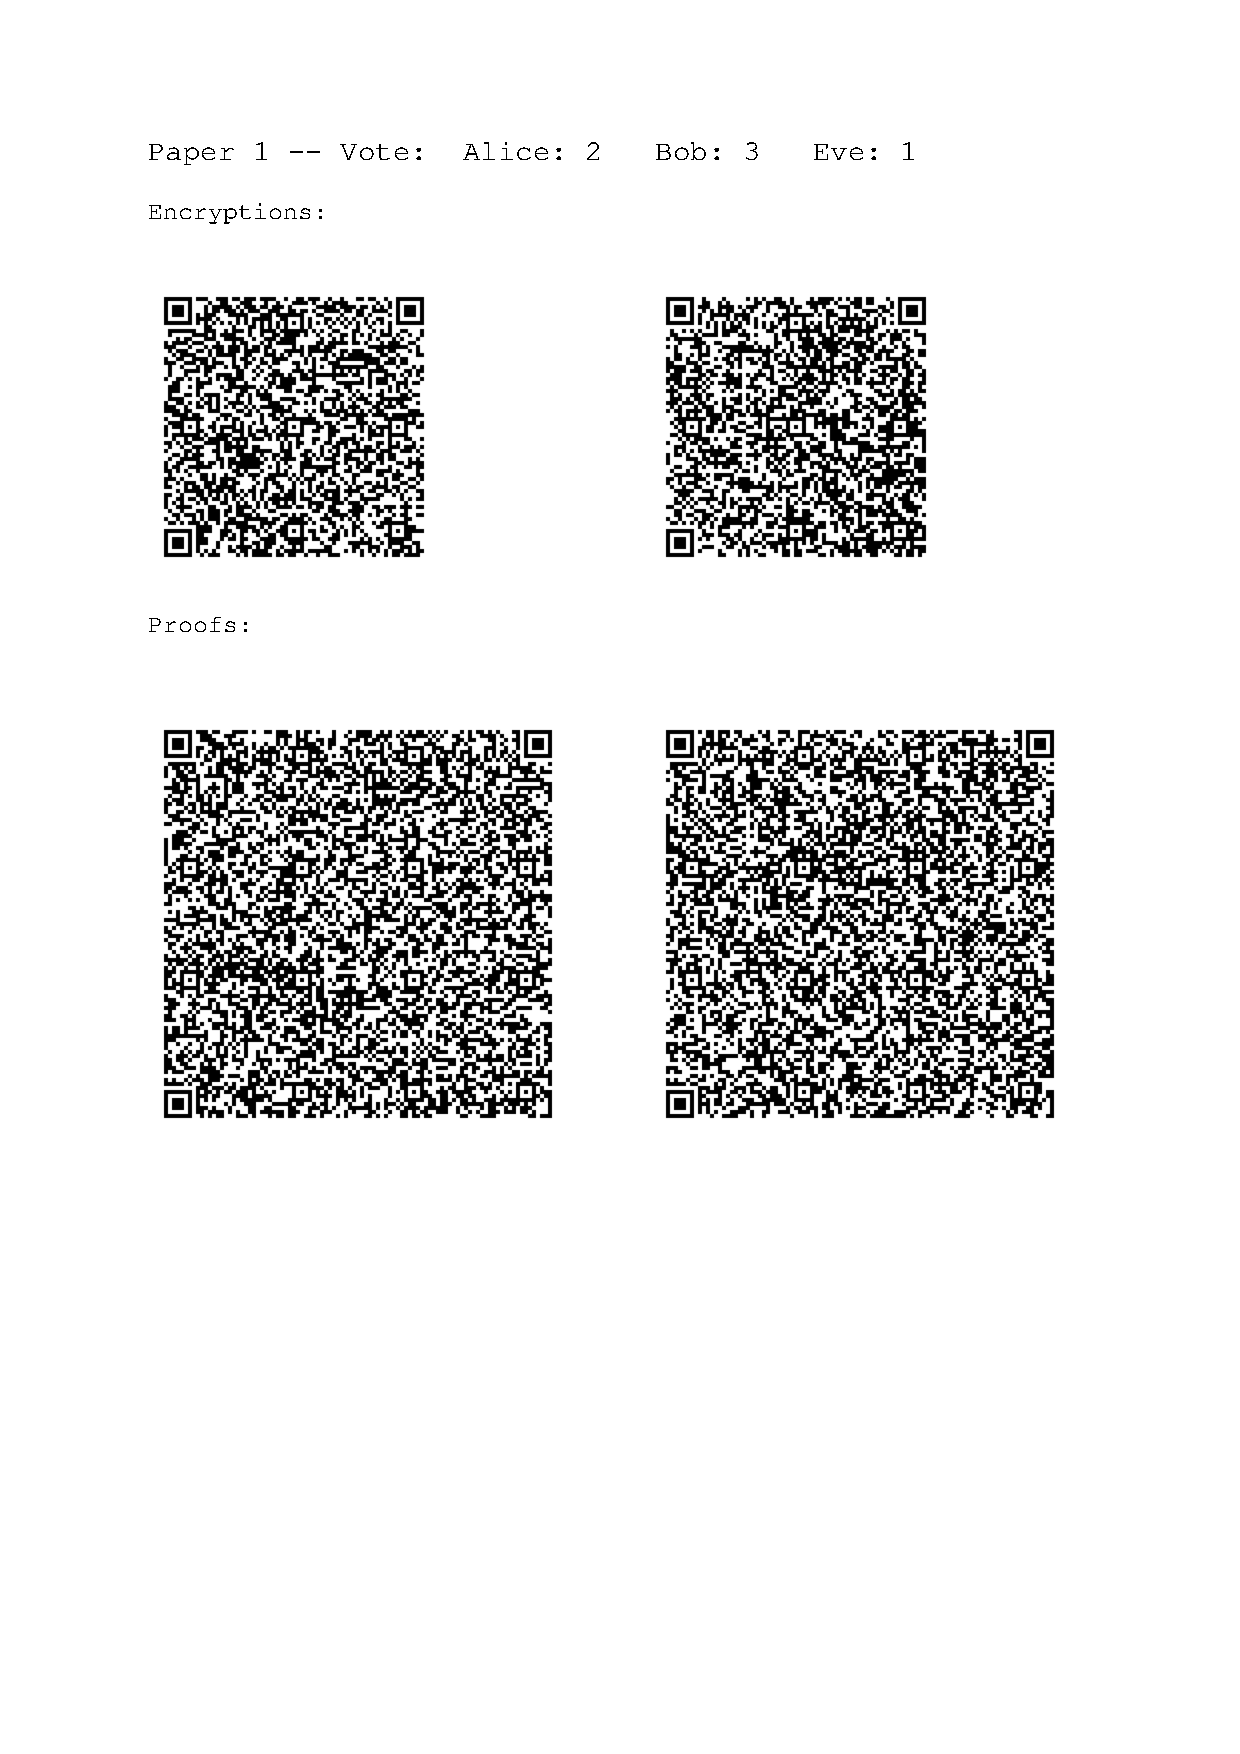
\includegraphics[scale=0.6, trim=2.5cm 10cm 3.1cm 0cm, clip=true]{paper1.pdf}
	\caption{$\Paper_1$: The top two QR codes contain encryptions of $a, b$ and $r_a, r_b$ respectively. The QR codes below contain proofs of plaintext knowledge.}
	\label{fig:prototype-paper1}
\end{figure}

\begin{figure}
	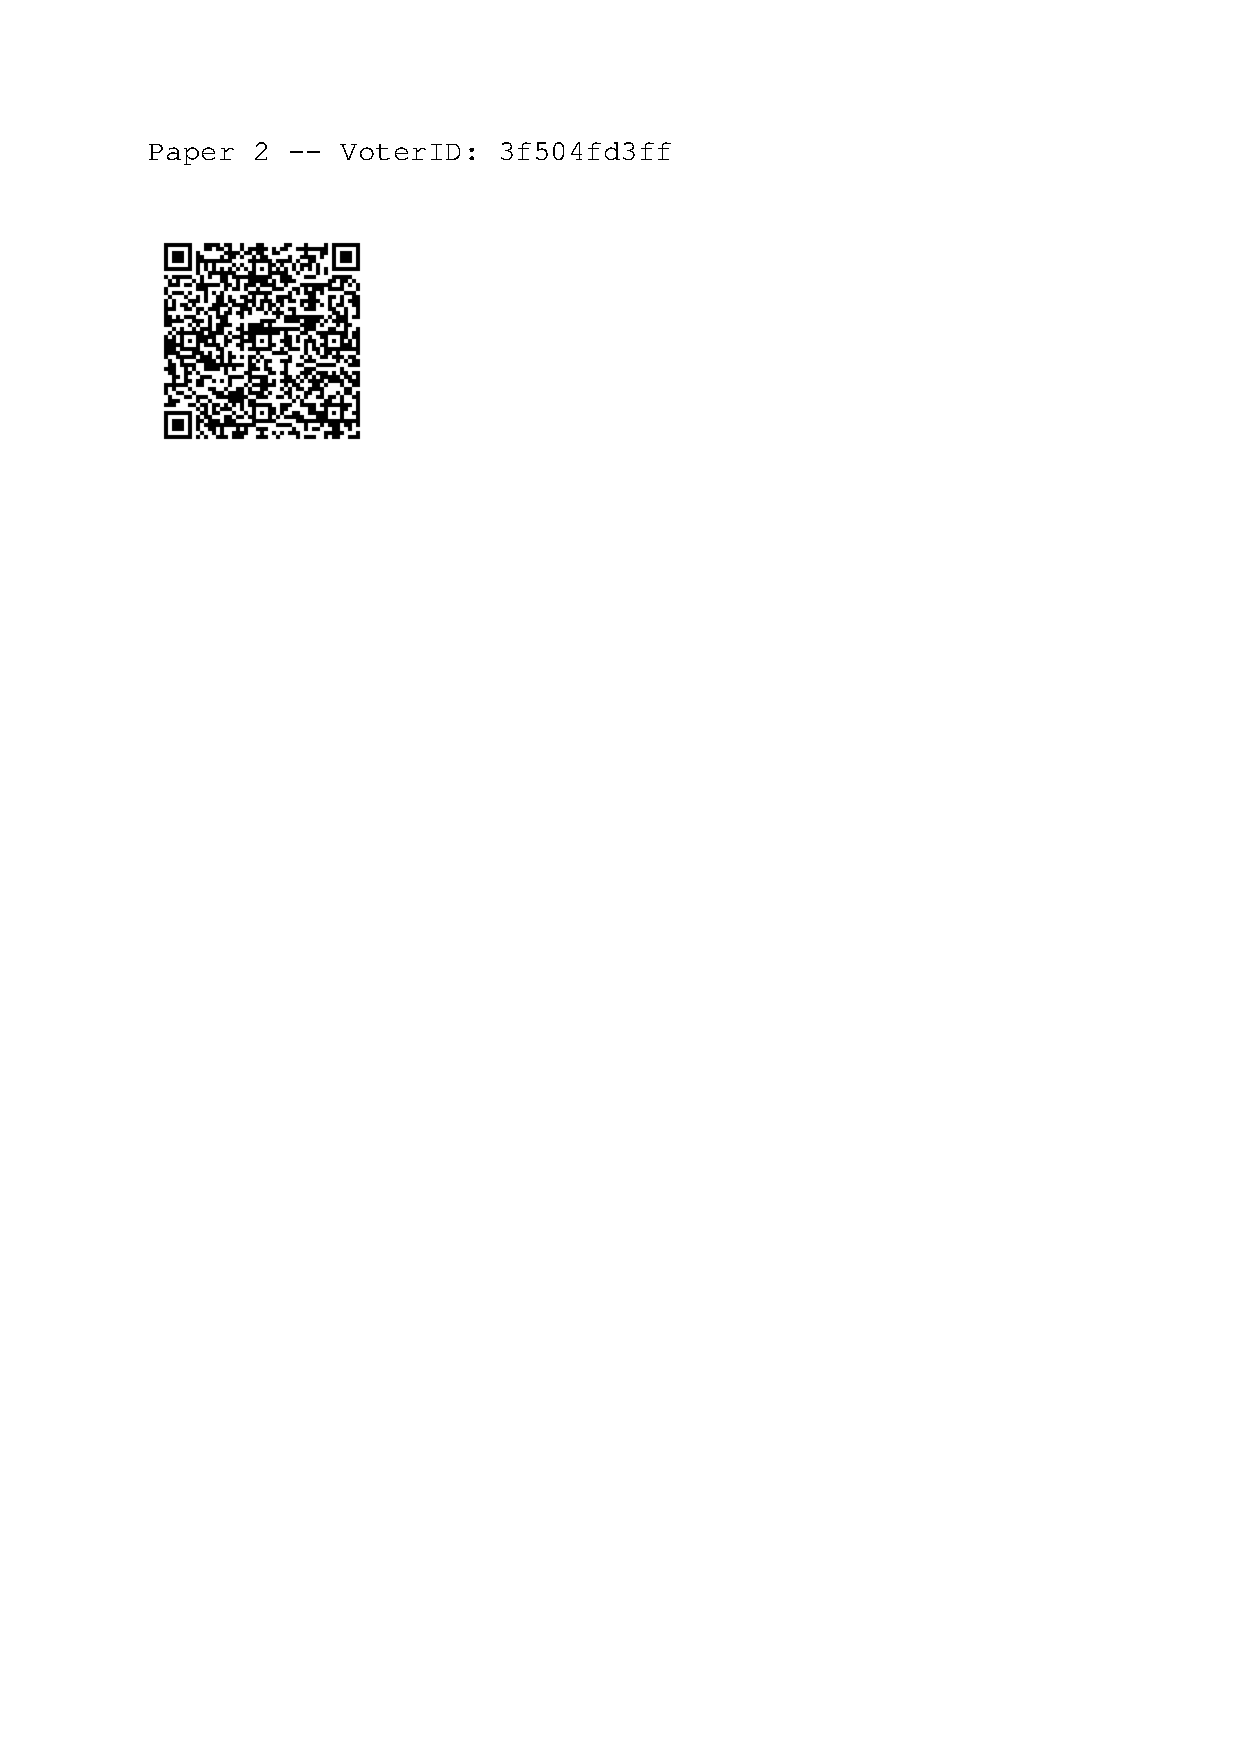
\includegraphics[scale=0.6, trim=0cm 22cm 4cm 0cm, clip=true]{paper2.pdf}
	\caption{$\Paper_2$: The QR code here contains an encryption of the $\VoterID$ on the paper, as well as a proof of encryption.}
		\label{fig:prototype-paper2}
\end{figure}

In an earlier version of the prototype, the encryptions and proofs were encoded as one large QR code; however, it was discovered that larger QR codes were unreliable when scanning. A real-world deployment would require careful testing to make sure QR codes can be successfully scanned in a variety of conditions.
The encryptions and proofs were encoded in base-64, with different group elements and integer powers delimited by the symbols \texttt{:} and \texttt{-}. As discussed above, more efficient encodings are possible; however, this did not noticeably impact functionality in our pilot testing. An example of the raw data encoded in the QR codes appears in Figure~\ref{fig:prototype-paper-raw}.

\begin{figure}
    \begin{verbnobox}[\tiny]
QKU6MknZMQmG/FqH/9a+ATNoqsLB9pzVBhH/kUiIVz0=:xma2+tThWCPkFTROOCmksG8sIKA2zhN/59Ij5Y8OjzI=
-xOwPjXhatRSV0IjbWNxS7lfsJxVFji1kGDKAj5rD4A0=
8oz3NyXNIB5aNsw/xYotQJQX0Z3oHnMseft/leng9Tk=:fLYrY2MF7cfTD6mQaOWbmhVX3nMtYOsZIB6PdlN+G2A=
-wJPk2/BnqF1vZccEmD3zXRWlzJjiPZ5YJ56PWLXBk24=:MGh1hNVjRZisPKMPtzcIVJUL9SoWl7S4X07MooSU8mw=
/MvJE05PV5zV0HueCHAogvrso40jii6UALTorCrn+GQ=:BJOSw5yRmTT6DlHOy0FNt4KUum64i4rhKoyQAduwnE0=
-rsddOzCGheFpTn51+Qu8vCENvk6aN+zCYMQjU5WRkhw=:KmE4z66IwiEsefzcGM0Vj7JCQpAykhyNSdkzKQKoBEI=
4vKuCmq8TnGohKlhxQBRX1jjC2qlgt2NtqZZReCNLXY=-8oz3NyXNIB5aNsw/xYotQJQX0Z3oHnMseft/leng9Tk=:
fLYrY2MF7cfTD6mQaOWbmhVX3nMtYOsZIB6PdlN+G2A=-YIvP27EA0rJBulVllYKbv52howw0XCrnaF5WzWjYrSo=
-pPNgXRxlV0cXl3YVWj3ZYSvo3BVmtxKJr7bbRqQB4QM=_4vKuCmq8TnGohKlhxQBRX1jjC2qlgt2NtqZZReCNLXY=
-wJPk2/BnqF1vZccEmD3zXRWlzJjiPZ5YJ56PWLXBk24=:MGh1hNVjRZisPKMPtzcIVJUL9SoWl7S4X07MooSU8mw=
-XleTY8eL6FzTrT5KHkgIMMUs6ZM74TneJIUv/6oytQM=-882097wkpA6H45H0LqfqHrLIcmbUdpask0Cr1bwCcwA=
4vKuCmq8TnGohKlhxQBRX1jjC2qlgt2NtqZZReCNLXY=-/MvJE05PV5zV0HueCHAogvrso40jii6UALTorCrn+GQ=:
BJOSw5yRmTT6DlHOy0FNt4KUum64i4rhKoyQAduwnE0=-cOc5/GqnHzdJJVR3hqcsNcQ7lXC21d8pcB4oo0hvtyA=
-VLazjpIPMuSWzF0hb3r1TWRi03Md+f2MimAkpYTKHQM=_4vKuCmq8TnGohKlhxQBRX1jjC2qlgt2NtqZZReCNLXY=
-rsddOzCGheFpTn51+Qu8vCENvk6aN+zCYMQjU5WRkhw=:KmE4z66IwiEsefzcGM0Vj7JCQpAykhyNSdkzKQKoBEI=
-ggyFWLx0Gv2YKbeVfwH7I12IlVl6Zc/ZEYh5yw1Uc0E=-5hto9LRlL1EwqLPfzLPFW2U85du/7cGv6d+x4A6YWQM=
    \end{verbnobox}
    \centering
    \caption{An example of the raw data encoded in the QR codes for $\Paper_1$ (line breaks inserted for readability). Upon close inspection, it is clear this could be compressed further.}
    \label{fig:prototype-paper-raw}
\end{figure}

\subsection{Benchmarks}
Practicality was a key focus in the implementation process, as many existing voting protocols such as JCJ~\cite{juels2010coercion} require $O(n^2)$ complexity to tally $n$ votes. Bearing in mind that a real-world use of the protocol may need to count millions of votes, we ran benchmarks for each of the major operations of \textit{Tally} (Algorithm~\ref{alg:tally}) using an Intel i7-10750H CPU. We used 2-out-of-3 secret sharing with other parameters randomised.

The below results include latency in socket communication on a local system but do not include latency across a network due to limitations in available hardware. Benchmarks were run using sets of automatically-generated votes, received using the raw data instead of the physical paper. We tested the following operations from \textit{Tally} (Algorithm~\ref{alg:tally}):

\begin{itemize}
    \item the first shuffle (Step~\ref{Step:MixCast})
    \item the first decryption (Step~\ref{Step:DecryptParams})
    \item the PET operations (Steps~\ref{Step:ECVotePEP} and~\ref{Step:ECMACPEP})
    \item the final shuffle (Step~\ref{Step:MixAccepted})
    \item the final decryption (Step~\ref{Step:DecryptVote})
    \item additionally, the time to finish the tally (that is, download the decrypted votes from the WBB)
\end{itemize}

Creating and submitting a single ballot took an average of 1.2 seconds. The results are summarised in Figure~\ref{fig:benchmarks}. We see that the prototype achieves roughly linear complexity in practice, with some variance at lower numbers of votes (likely due to the communication overhead between trustees). The vast majority of processing time was spent in the plaintext equivalence test; this makes sense as it is quite a complex protocol (see Algorithm~\ref{prot:PEP}). The cost of PETs is a known issue in the literature, with older protocols requiring $O(n^2)$ PET procedures and thus being known to be impractical~\cite{juels2010coercion}.
\begin{figure}
        \begin{tabular}{l|llllll}
        Vote count & First shuffle & First dec. & PET & Final shuffle & Final dec. & Tallying \\ \hline
        500             & 2.33 s             & 1.95 s                & 11.2 s   & 1.5 s              & 0.94 s                & 0.66 s        \\
        1000            & 6.21 s             & 4.76 s                & 31.5 s   & 4.35 s             & 2.38 s                & 1.88 s        \\
        5000            & 20.9 s             & 17.6 s                & 117 s    & 16.9 s             & 9.92 s                & 7.40 s       
        \end{tabular}
    \centering
    \caption{Benchmark results for each major step of \textit{Tally} on varying numbers of votes.}
    \label{fig:benchmarks}
\end{figure}

We also tested the implementation of the verifiable shuffle, since this is also a complex protocol that can be expensive (see Section~\ref{sec-shuffle}). With 100000 rows of 6 ciphertexts, the proof was generated in 38.3 seconds and verified in 26.4 seconds (without network latency). This suggests that the protocol would successfully scale to the order of millions of votes given more powerful hardware and a suitably-fast local area network, completing in the order of minutes to at most hours.

\subsection{Real-world pilot}
We ran a real-world pilot of the protocol with human voters, using three trustees and the WBB running on the same server for simplicity. A small number of volunteers were asked to rank candidates Alice, Bob, and Eve; the example votes from Section~\ref{sec:cast-ballot} were taken from this pilot. Seven preferential votes (ranking candidates 1, 2, and 3 where 1 is the highest preference) were submitted and physically mailed to the author, acting as the EC. Five of these ballots were successfully scanned, with the other two being lost due to errors in the receiving process such as accidentally destroying pieces of paper. This provided a nice opportunity to test the verification procedures: five voters used the verification program, and one of those voters discovered that their vote had been excluded from the count.

While this is not close to a full usability study or test in a realistic setting, the small-scale pilot demonstrates that voters can successfully use the system, that the system is complete and functional, and that simple problems can be detected by voters.
\footnote{For avoidance of doubt, Eve won in a landslide.}
\newpage
\section{Future work \& conclusion}\label{sec-conclusion}
We have presented a novel cryptographic protocol for verifiable remote voting. In this section we discuss future work stemming from the development of the protocol, and provide some concluding remarks.
\subsection{Future work}
The protocol we present emphasises verifiability but does not attempt to provide accountability, nor any defence against denial-of-service and other malicious attempts to construct problems when there were none. For example, one could generate and physically post fake ballots with someone else's $\VoterID$. This will not successfully forge a vote, but will flag the $\VoterID$ as having encountered a problem. While this does not defeat verifiability, it would (detectably) cause votes to be discounted and would give an indication of attempted fraud. A practical defence here is to make $\VoterID$s hard to guess, although this needs to be done with some care to avoid clash attacks (whereby two voters are persuaded that they have the same $\VoterID$).

A key assumption the protocol makes is that the client and EC are not both compromised. In an ideal world, people would download, compute a checksum, and compile an open-source voting app from an independent source they  trusted. In practice, voters generally get instructions and software from the same authority that will be receiving their votes. This is an important practical issue for true security of our scheme. However, as previously discussed most existing verifiable voting systems (particularly those based on code voting) fall victim to the same problem.

Several possible extensions discussed in Section~\ref{sec-extensions} provide tangible benefits to the security and privacy of the protocol, but at a significant cost in terms of user experience. A useful avenue of work would be to find better compromises, allowing access to the strongest possible security and privacy guarantees in an accessible and error-resistant manner.

Before deploying the voting system in a real-world context, more extensive user testing would be needed. Formal research analysing the understanding and ability of many different potential voters to use the system should be performed, as well as a professional security audit on the codebase itself. A graphical user interface (rather than a command-line interface) would go a long way to achieving real-world practicality. Further, it is unclear how many voters have access to a printer---this would be a valuable insight to have. For voters who do not have a printer, it would be useful to study whether these voters would be comfortable using \eg a public library printer to create their ballots, and to consider whether this is a realistic security and/or privacy risk.

Finally, the protocol only achieves \textbf{passive} receipt freeness. While this is much stronger than the properties achieved in similar existing work, this is a significant limitation that would benefit from further research.
\subsection{Conclusion}
We have developed a significant step forward in the design of verifiable remote voting protocols. Focusing on easy cast-as-intended verifiability with the voter visually inspecting a paper ballot and scrutineers ensuring the correctness of constructed ballots, we augment existing postal voting procedures with passive receipt-freeness (assuming access to an untappable channel) and a strong form of verifiability.

While our protocol does not provide universal verifiability, we require only that we assume \textbf{either} the voter's device \textbf{or} the postal service and electoral commission are honest---or at least, are not actively colluding. This is a reasonable trade-off in practice, and our work is the first that can provide all of these strengths simultaneously.

We reviewed the theoretical background underpinning cryptographic voting protocols, and using a minor variant of existing definitions formally proved verifiability and privacy properties of our protocol. We developed a functioning prototype implementation for the protocol, and tested it both under large-scale simulated loads and at a smaller scale in real-world conditions, demonstrating the protocol's viability. 

Verifiable remote voting is far from a solved problem, and is considered by many to be one of the hardest open problems in applied cryptography. We have provided but another step towards this goal, and we hope that the area continues to mature well into the future.
\newpage
\section{References}
\bibliographystyle{unsrt}
\bibliography{papers}
\newpage
% \appendix
% \newpage
% \section{Implementation algorithms}\label{app-algorithms}
% GitHub repository: \url{https://github.com/eleanor-em/papervote/}
% \begin{algorithm} 	\caption{Generate Pedersen parameters}
% \textbf{Input:} a seed value $\mathit{seed}$ and a number of generators to produce $n$\\
% \textbf{Output:} verifiable generators $g$, $h$, $h_1, \ldots, h_n$
% \begin{algorithmic}[1]
%     \State  $\mathit{counter} \gets 0$
%     \State  $g \gets$ SHA-512$(\mathit{seed}, \mathit{counter})$
%     \State  $\textit{counter} \gets \mathit{counter} + 1$
%     \State  $h \gets$ SHA-512$(\mathit{seed}, \mathit{counter})$
%     \For {$i=1$ to $n$}
%         \State $h_i \gets$ SHA-512$(\mathit{seed}, \mathit{counter})$
%         \State  $\textit{counter} \gets \mathit{counter} + 1$
%     \EndFor
%     \State return $(g, h, h_1, \ldots, h_n)$
% \end{algorithmic}
% \end{algorithm}
% \VTNote{I think you need to check $h_i$ is in the group generated by $g$, unless of course you're in a setting that uses the whole group.  There's a precise algorithm in the final version of the 'how not to prove your election outcome' paper.  And a ref to the NIST standard.}

% \begin{algorithm}\caption{Joint ElGamal key generation}
% \textbf{Input:} public ElGamal parameters $(\mathbb{G}, g, q)$, a number of trustees $n$, and a threshold for decryption $k < n$\\
% \textbf{Output:} jointly generated public key $Y$ and secret key shares $x_i$ for trustee $T_i$ (or $\bot$ on failure)
% \begin{algorithmic}[1]
%     \State  $T_i$: $a_0 \gets_R \mathbb{Z}_q$
%     \For {$j=1$ to $k - 1$}
%         \State $T_i$: $a_j \gets_R \mathbb{Z}_q$
%     \EndFor
%     \State $T_i$: $f_i(x)\gets a_0 + a_1 x + a_2 x^2 + \ldots + a_{k-1} x^{k-1}$
%     \For {$j=0$ to $k-1$}
%         \State $T_i$: $C_{ij} \gets g^{a_j}$
%         \State $T_i\rightarrow T_j$: $C_{ij}$
%     \EndFor
%     \For {$j = 0$ to $k-1$}
%         \State $T_i\rightarrow T_j$: $f_i(j)$
%         \State $T_j$: check that $f_i(j)=\prod_{l=0}^{k-1}\left(C_{il}\right)^{jl}$ (otherwise output $\bot$)
%     \EndFor
%     \State $T_i$: $x_i \gets \prod_{j=0}^{k-1} f_j(i)$
%     \State $Y \gets \prod_{i=0}^{k-1} C_{i0}$
%     \State $T_i$: return $(Y, x_i)$
% \end{algorithmic}
% \end{algorithm}
% \VTNote{I think in Alg 20 you want double indices on the polynomial coefficients.  That is, $a_0$ should be $a_{i0}$ and so on.  Then at line 6 you'll have $C_{ij} \gets g^{a_{ij}}$ and everything will work out nicely.}
\end{document}
